\section{Prototypical materials}
Firstly, one pretends to present the structure of the materials used for the respective calculations. A list of the materials can be found in table \ref{tab:compounds}.
%% Tabela 1.1 listando a quantidade de materiais cálculados e se são bidimensionais ou tridimensionais
\begin{table}[h]
    \small
    \setlength{\tabcolsep}{5pt} % Adjust cell padding
    \renewcommand{\arraystretch}{1.2} % Adjust row height
    \centering
    \caption{Table containing all the compounds simulated in this study and the classification of their respective structures into the categories of three-dimensional and two-dimensional.}
    \label{tab:compounds}
    \begin{tabular}{c c c}
        \hline
        \hline
        \textbf{Element} & \textbf{Dimensionality} & \textbf{Structure Type}  \\
        \hline
        AlN & 2D& \\
        GaP & 2D& \\
        GaN & 2D& \\
        GaP & 2D& \\
        BN & 2D& \\
        BP & 2D& \\        
        GeC & 2D & \\
        SiC & 2D & \multirow{-8}{*}{Honeycomb} \\
        AlN & 3D& \\
        GaP & 3D& \\
        GaN & 3D& \\
        Ge & 3D & \\
        GaAs & 3D & \\
        InP & 3D & \\
        Si & 3D & \multirow{-7}{*}{Zincblend} \\
        \hline
        \hline
    \end{tabular}
\end{table}

To define the structures, one used the $VASP$ $POSCAR$ file, specifying the lattice vectors and the precise position of each atom relative to its constituent lattice vector. For clarity, listing \ref{lst:si_poscar} presents the $Si$ $POSCAR$ file along with explanatory comments indicating the meaning of each line.
\newpage
\begin{lstlisting}[language=bash,caption={POSCAR file for Si},linewidth=\linewidth,label={lst:si_poscar}]
Si # Comment line                                      
   5.439 # Scaling factor 
     0.50    0.00    0.50 # Lattice vector a1
     0.50    0.50   -0.00 # Lattice vector a2
     0.00    0.50    0.50 # Lattice vector a3
   Si # Ion Specie
     2 # Ion Number
Direct
#   x1   y1    z1 
  0.00  0.00  0.00 # atom position r1 = x1a1 + y1a2 + z1a3  
#   x2   y2    z2
  0.25  0.25  0.25 # atom position r2 = x2a1 + y2a2 + z2a3
\end{lstlisting}

The listing \ref{lst:si_poscar} defines a unit cell that is infinitely repeated to simulate a crystal. Figure \ref{fig:si_st_rep} elucidates how the repetition of the unit cell forms the crystalline structure.

\begin{figure}[!ht]
    \begin{subfigure}[b]{.5\textwidth}%
        \centering
        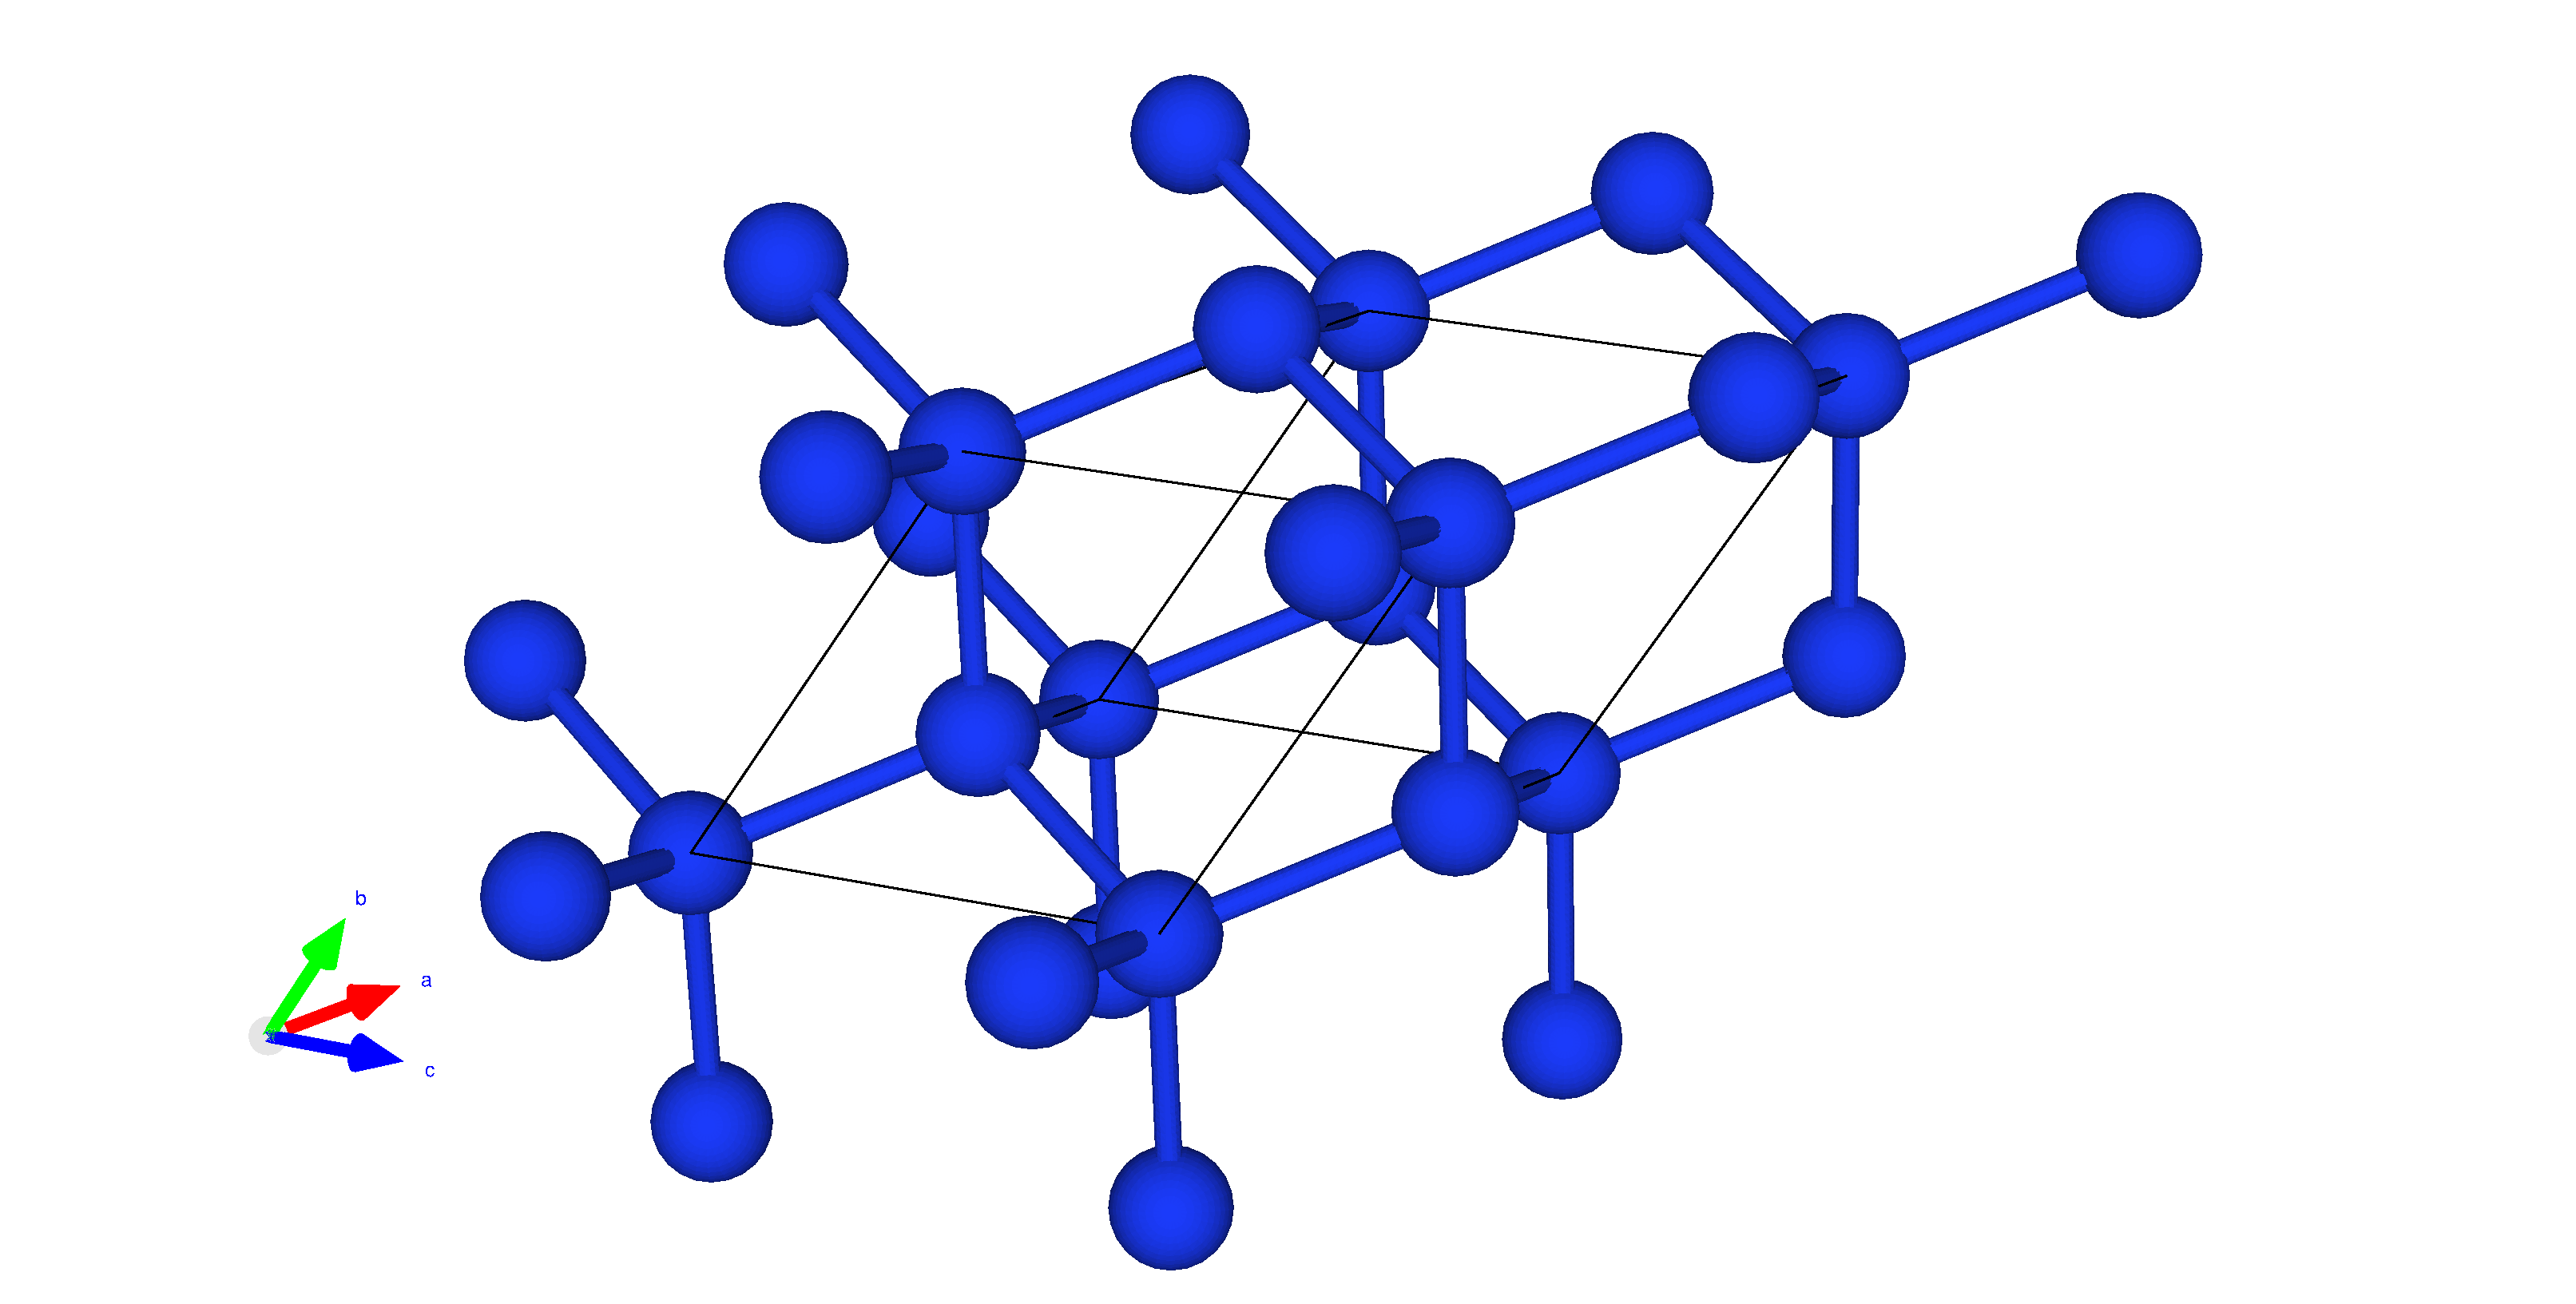
\includegraphics[width=\linewidth]{images/si_st.eps}
        \caption{Silicon Unit Cell}
    \end{subfigure}%
    \begin{subfigure}[b]{.5\textwidth}%
        \centering
        \includegraphics[width=\linewidth]{images/si_st_bc.eps}
        \caption{Silicon Super Unit Cell.}
    \end{subfigure}%
    \caption{Comparison between the silicon unit cell and a super unit cell to elucidate how the repetition of one unit cell forms the crystalline structure.}
    \label{fig:si_st_rep}
\end{figure}

An important point to consider is that the calculations replicate the pattern in three dimensions. Therefore, we need to model two-dimensional compounds as three-dimensional ones in order to perform the calculations. For this purpose, we model the system as the repetition of atomic layers separated by a significant distance, such as $L = 20,\text{\AA}$, with the aim of avoiding interactions between the layers. This is illustrated in figure \ref{fig:sic_st_bc}.

\begin{figure}[!ht]
        \centering
        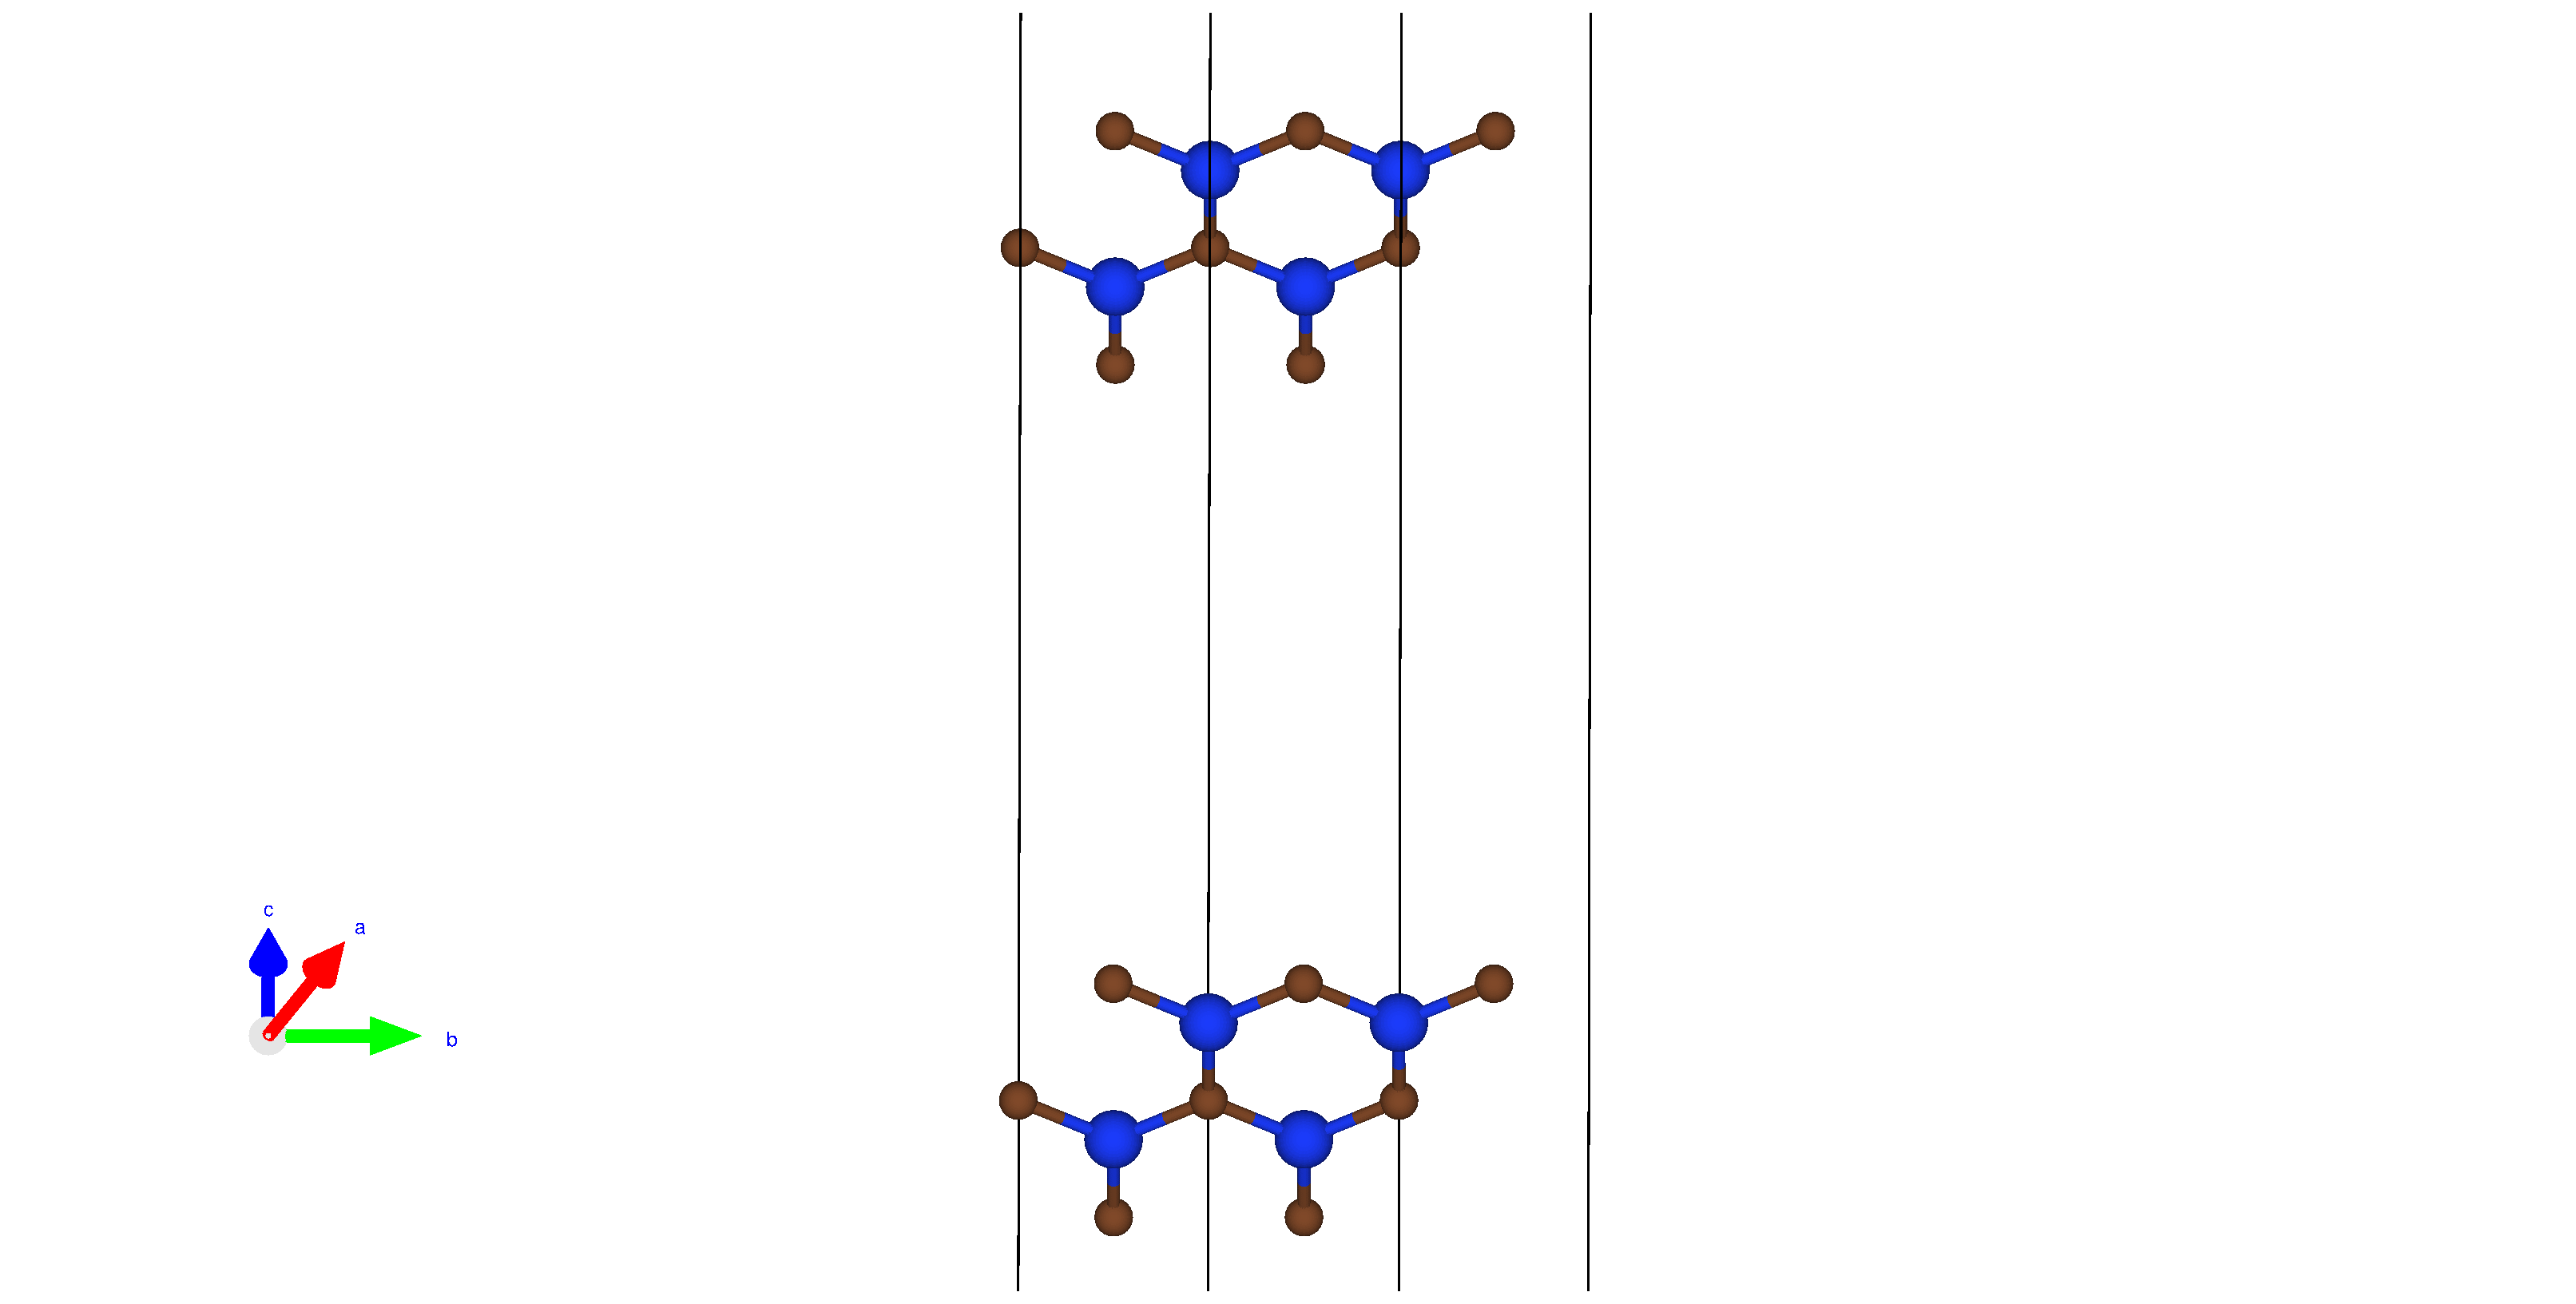
\includegraphics[width=\linewidth,height=7cm]{images/sic_st_bc.eps}
        \caption{Structure of 2D SiC. It is useful to understand how one simulates 2D materials using 3D crystal structures.}
        \label{fig:sic_st_bc}
\end{figure}


Thus, with the assistance of the VESTA software, figures \ref{fig:2d_materials_structure} and \ref{fig:3d_materials_structure} were generated, displaying the structures of all the materials simulated in this study.

\begin{figure}[htb]
    \centering % <-- added
\begin{subfigure}{0.3\textwidth}
  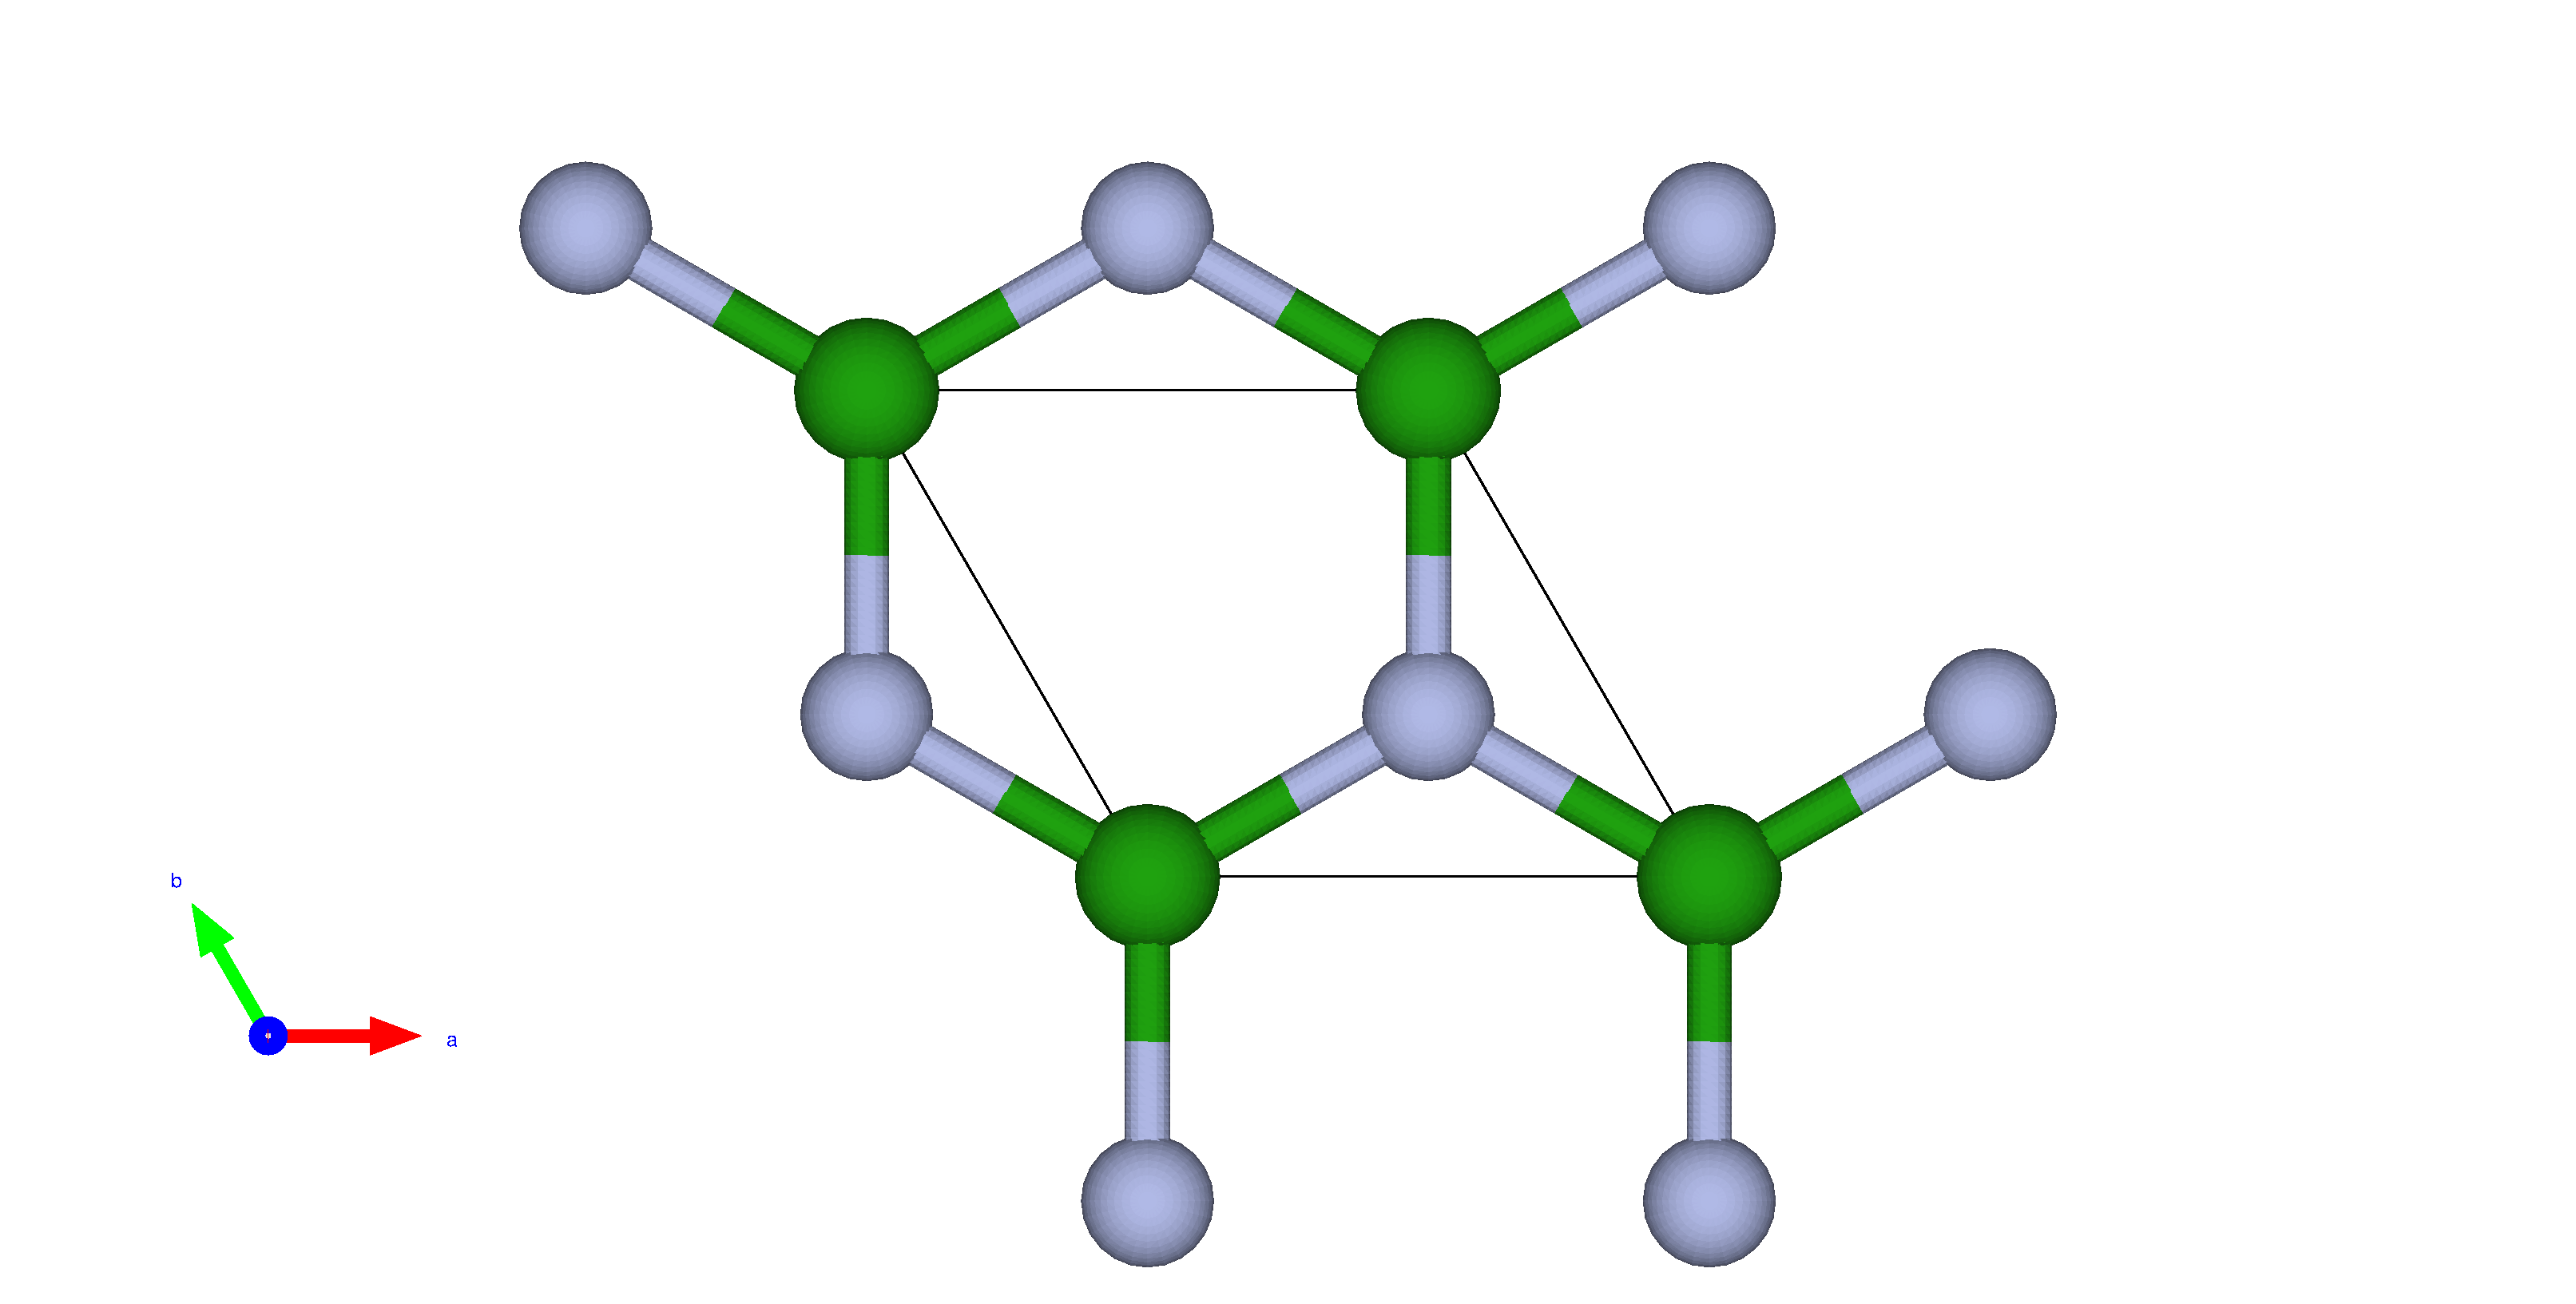
\includegraphics[width=\linewidth]{images/bn_st_2d.eps}
  \caption{BN}
\end{subfigure}\hfil % <-- added
\begin{subfigure}{0.3\textwidth}
  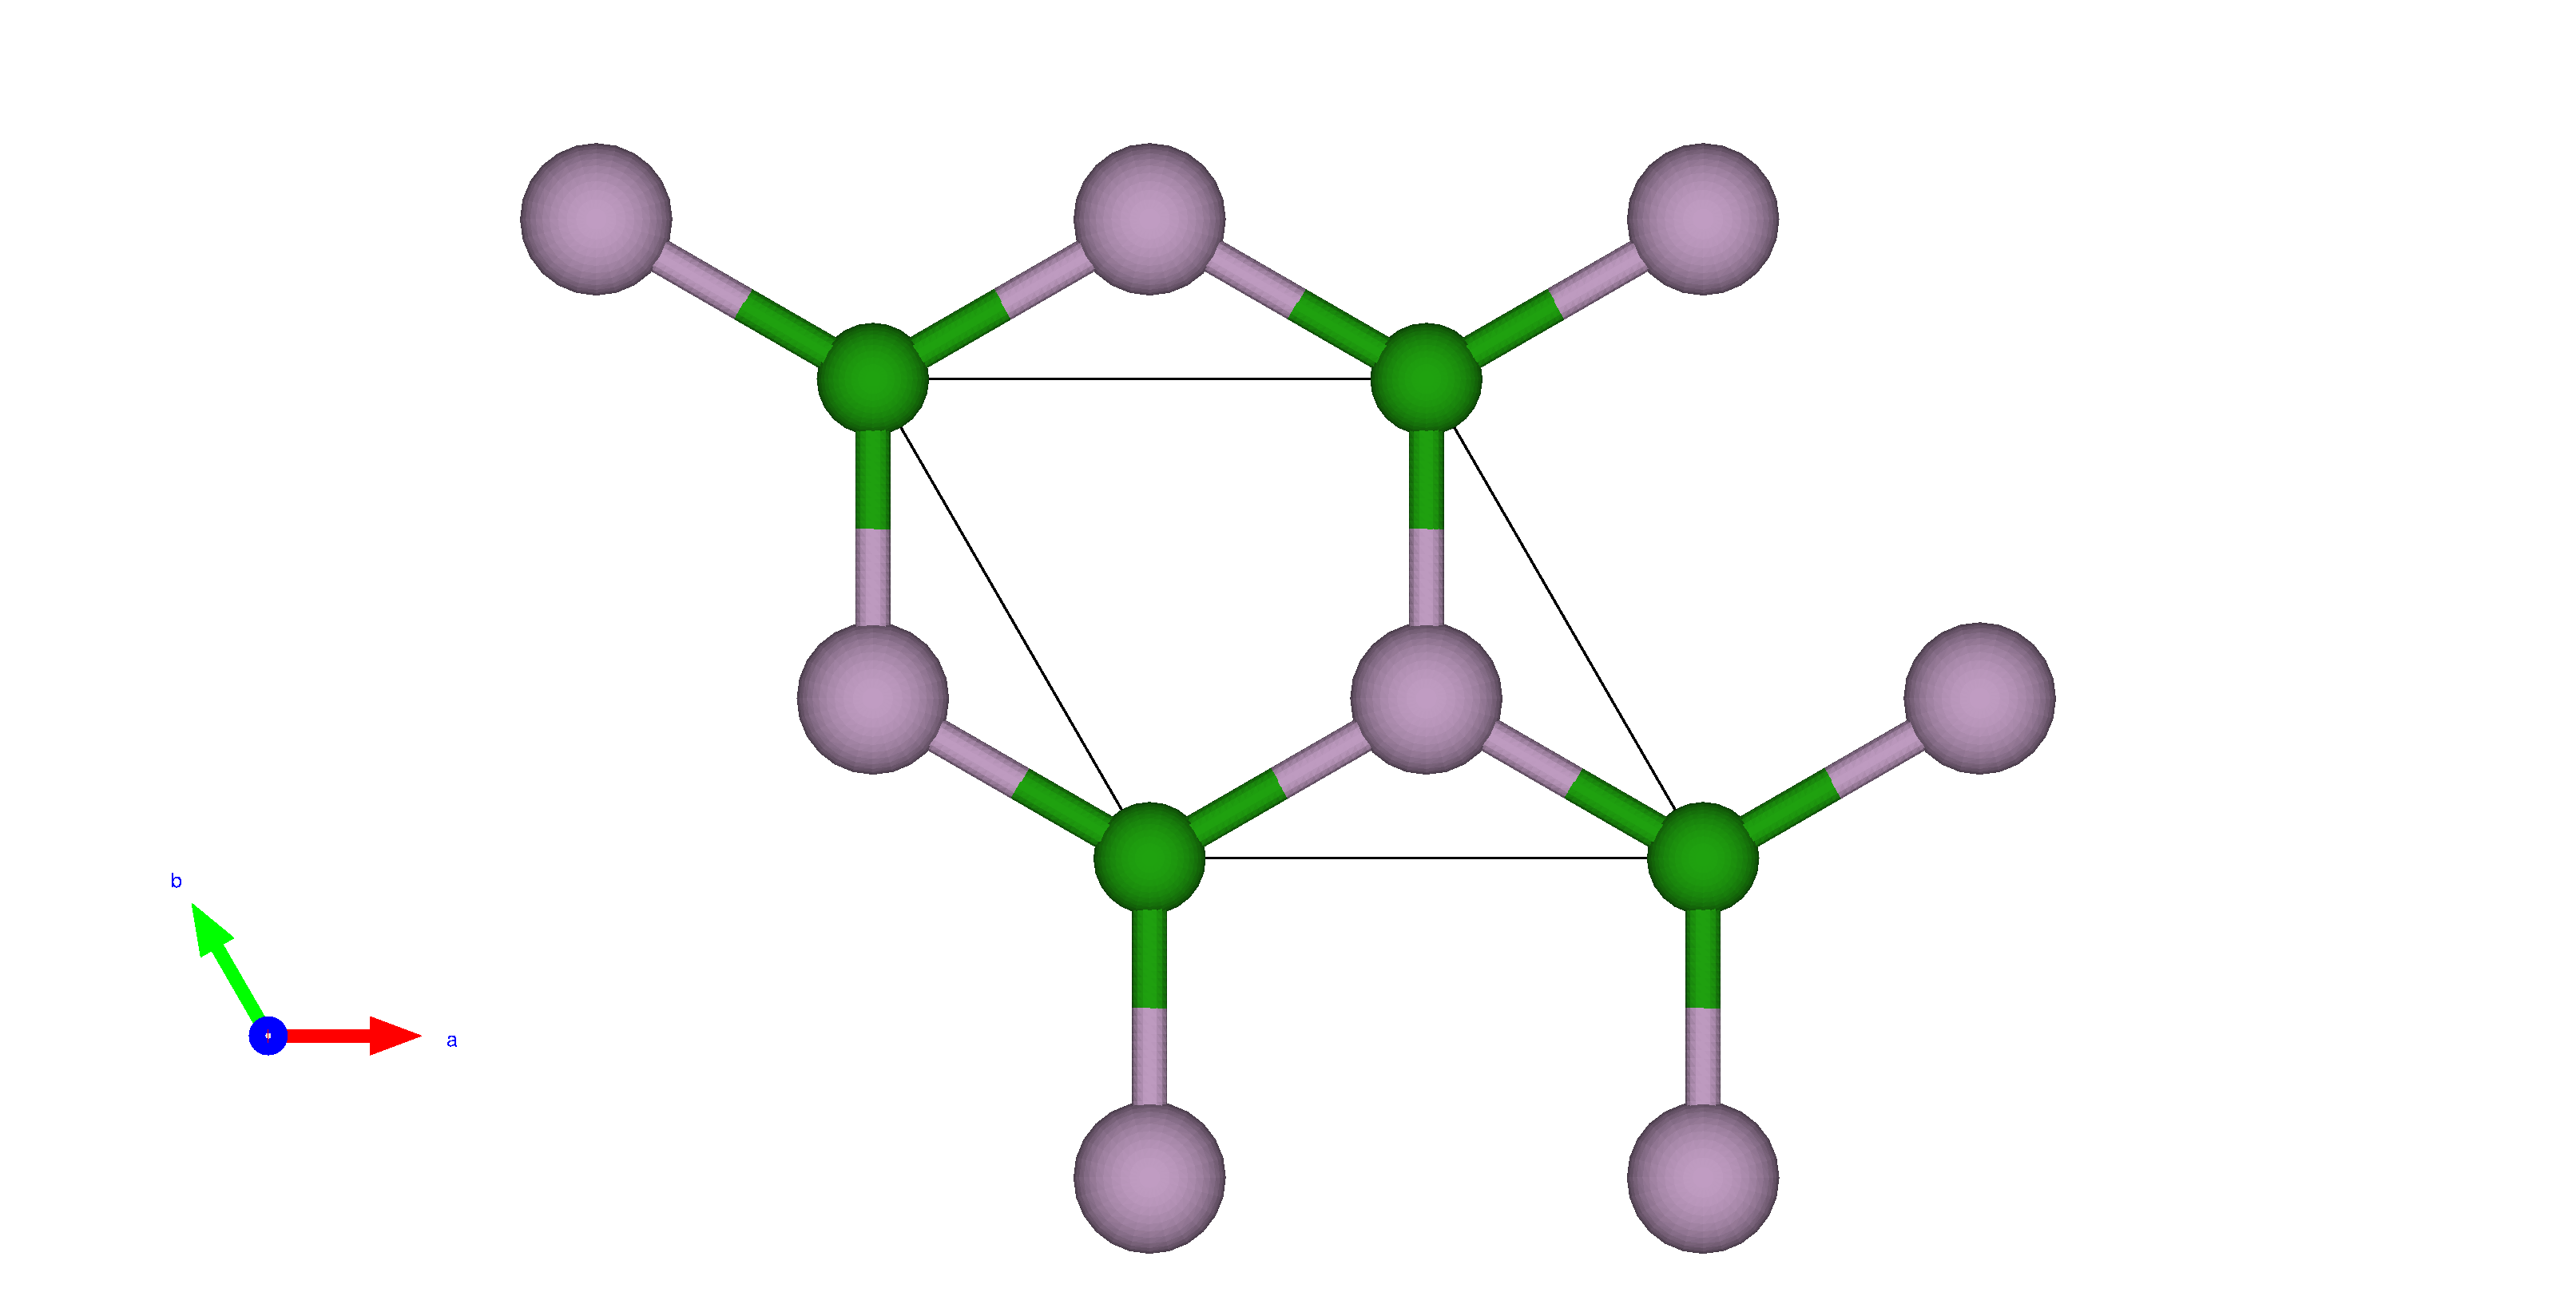
\includegraphics[width=\linewidth]{images/bp_st_2d.eps}
  \caption{BP}
\end{subfigure}\hfil % <-- added
\begin{subfigure}{0.3\textwidth}
  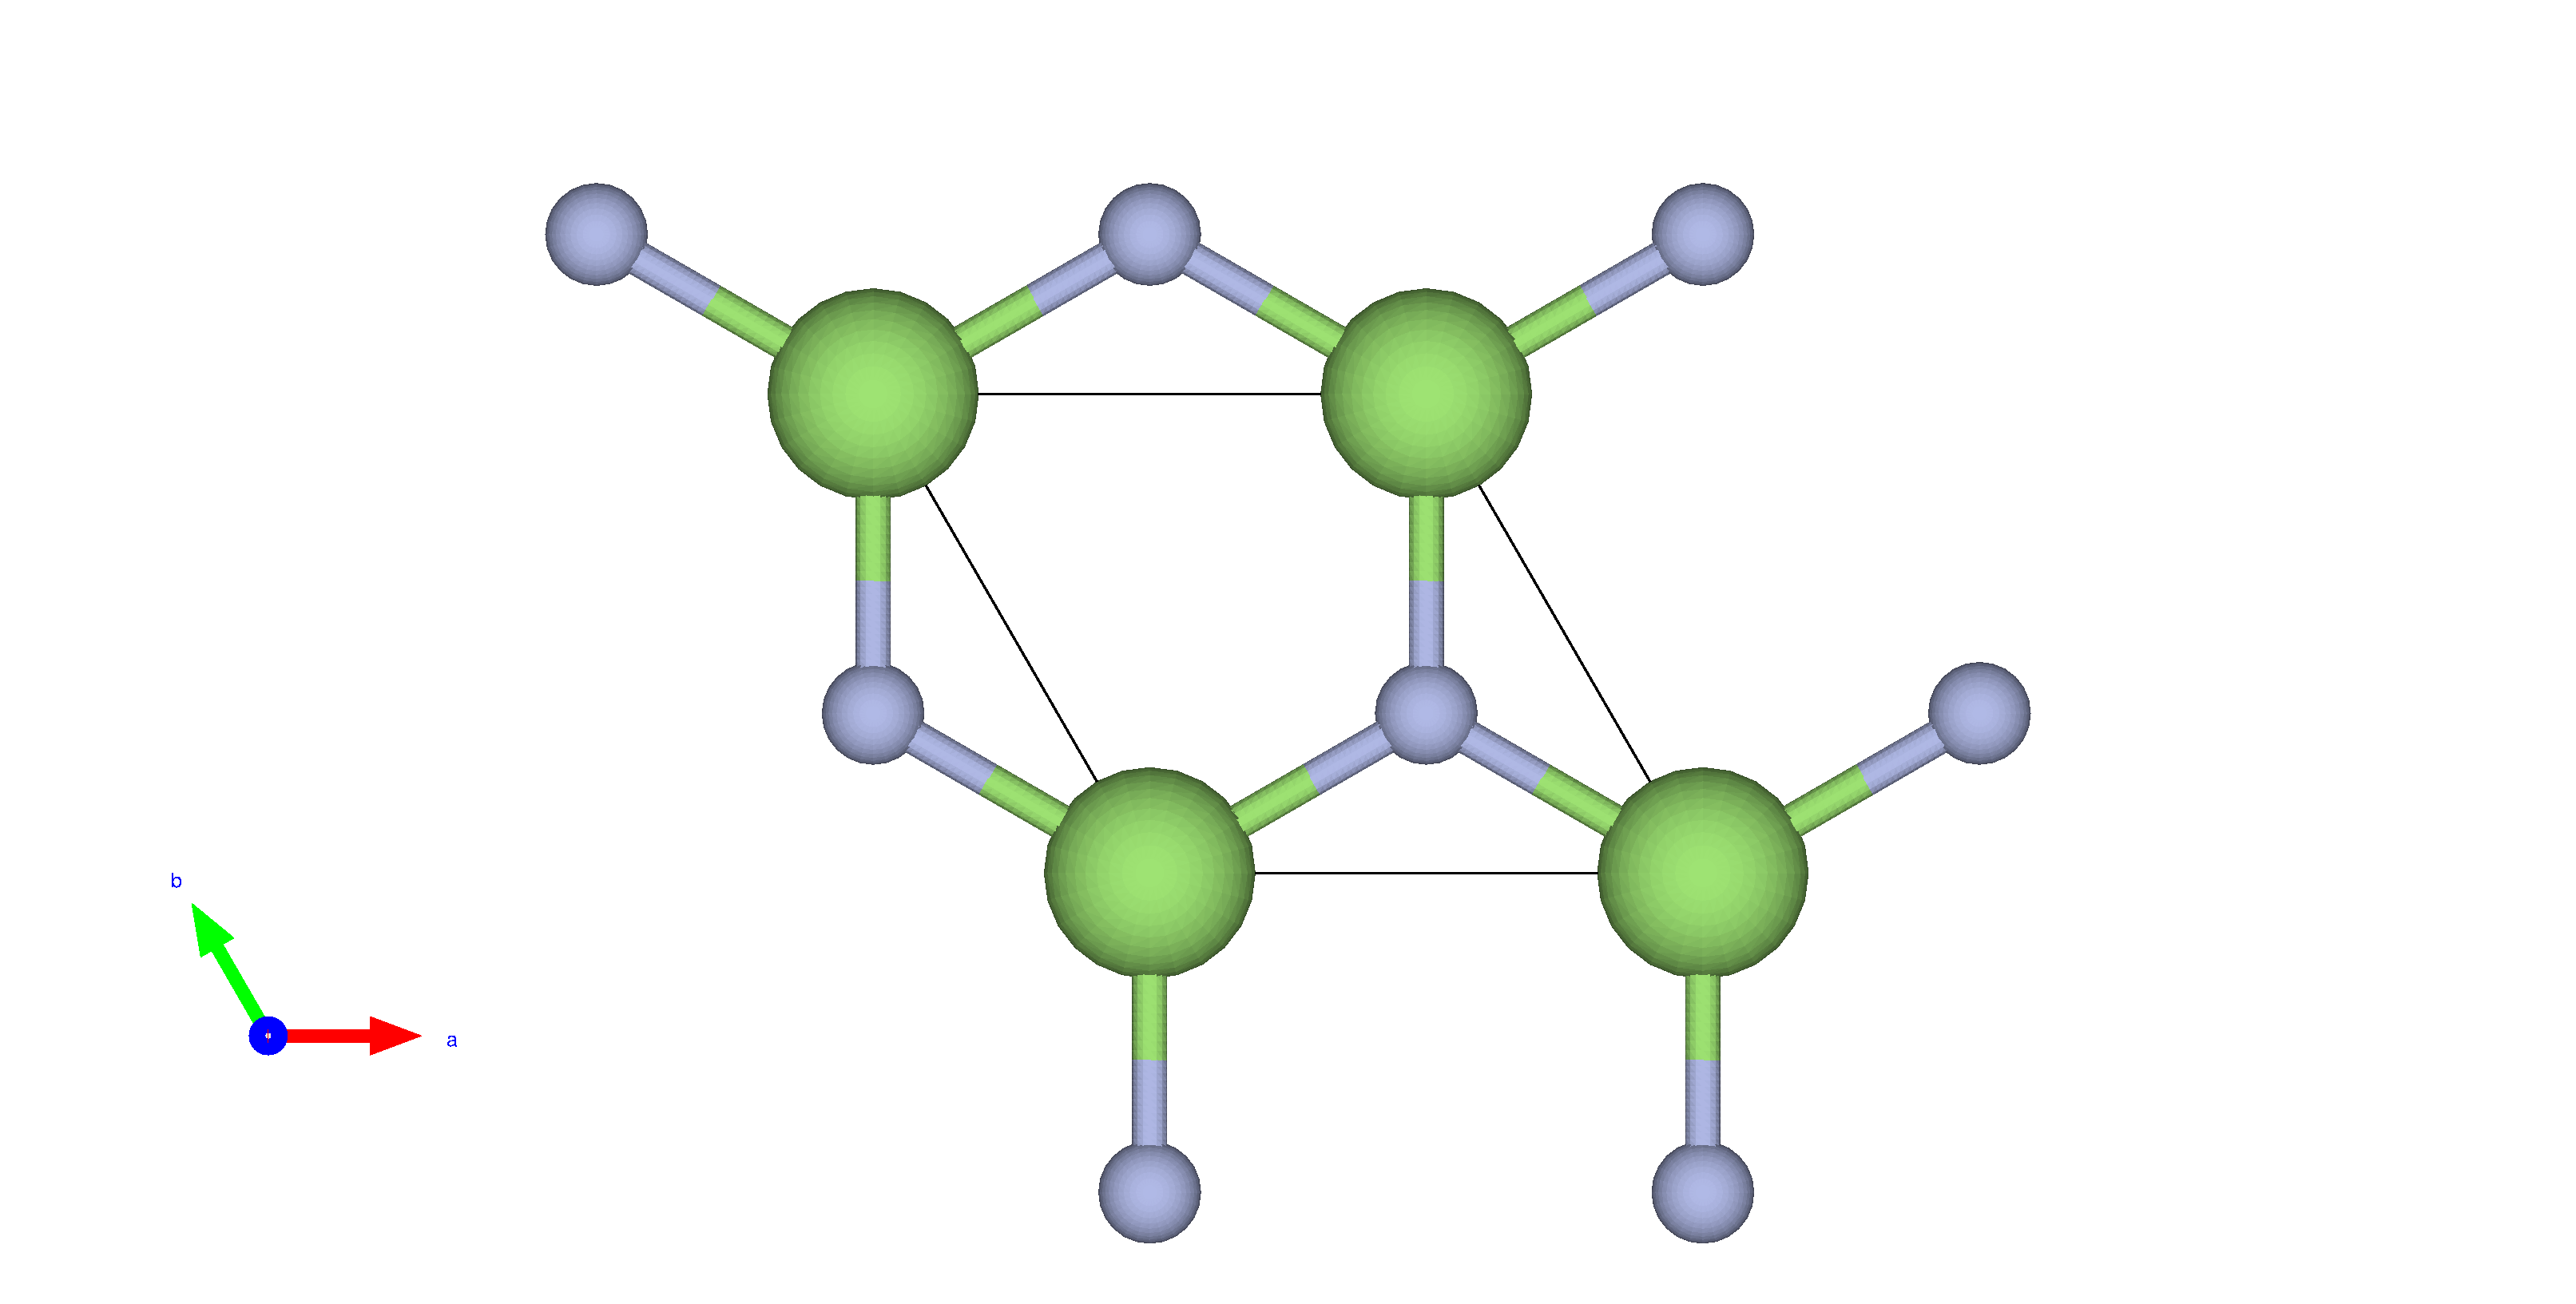
\includegraphics[width=\linewidth]{images/gan_st_2d.eps}
  \caption{GaN}
\end{subfigure}

\medskip
\begin{subfigure}{0.3\textwidth}
  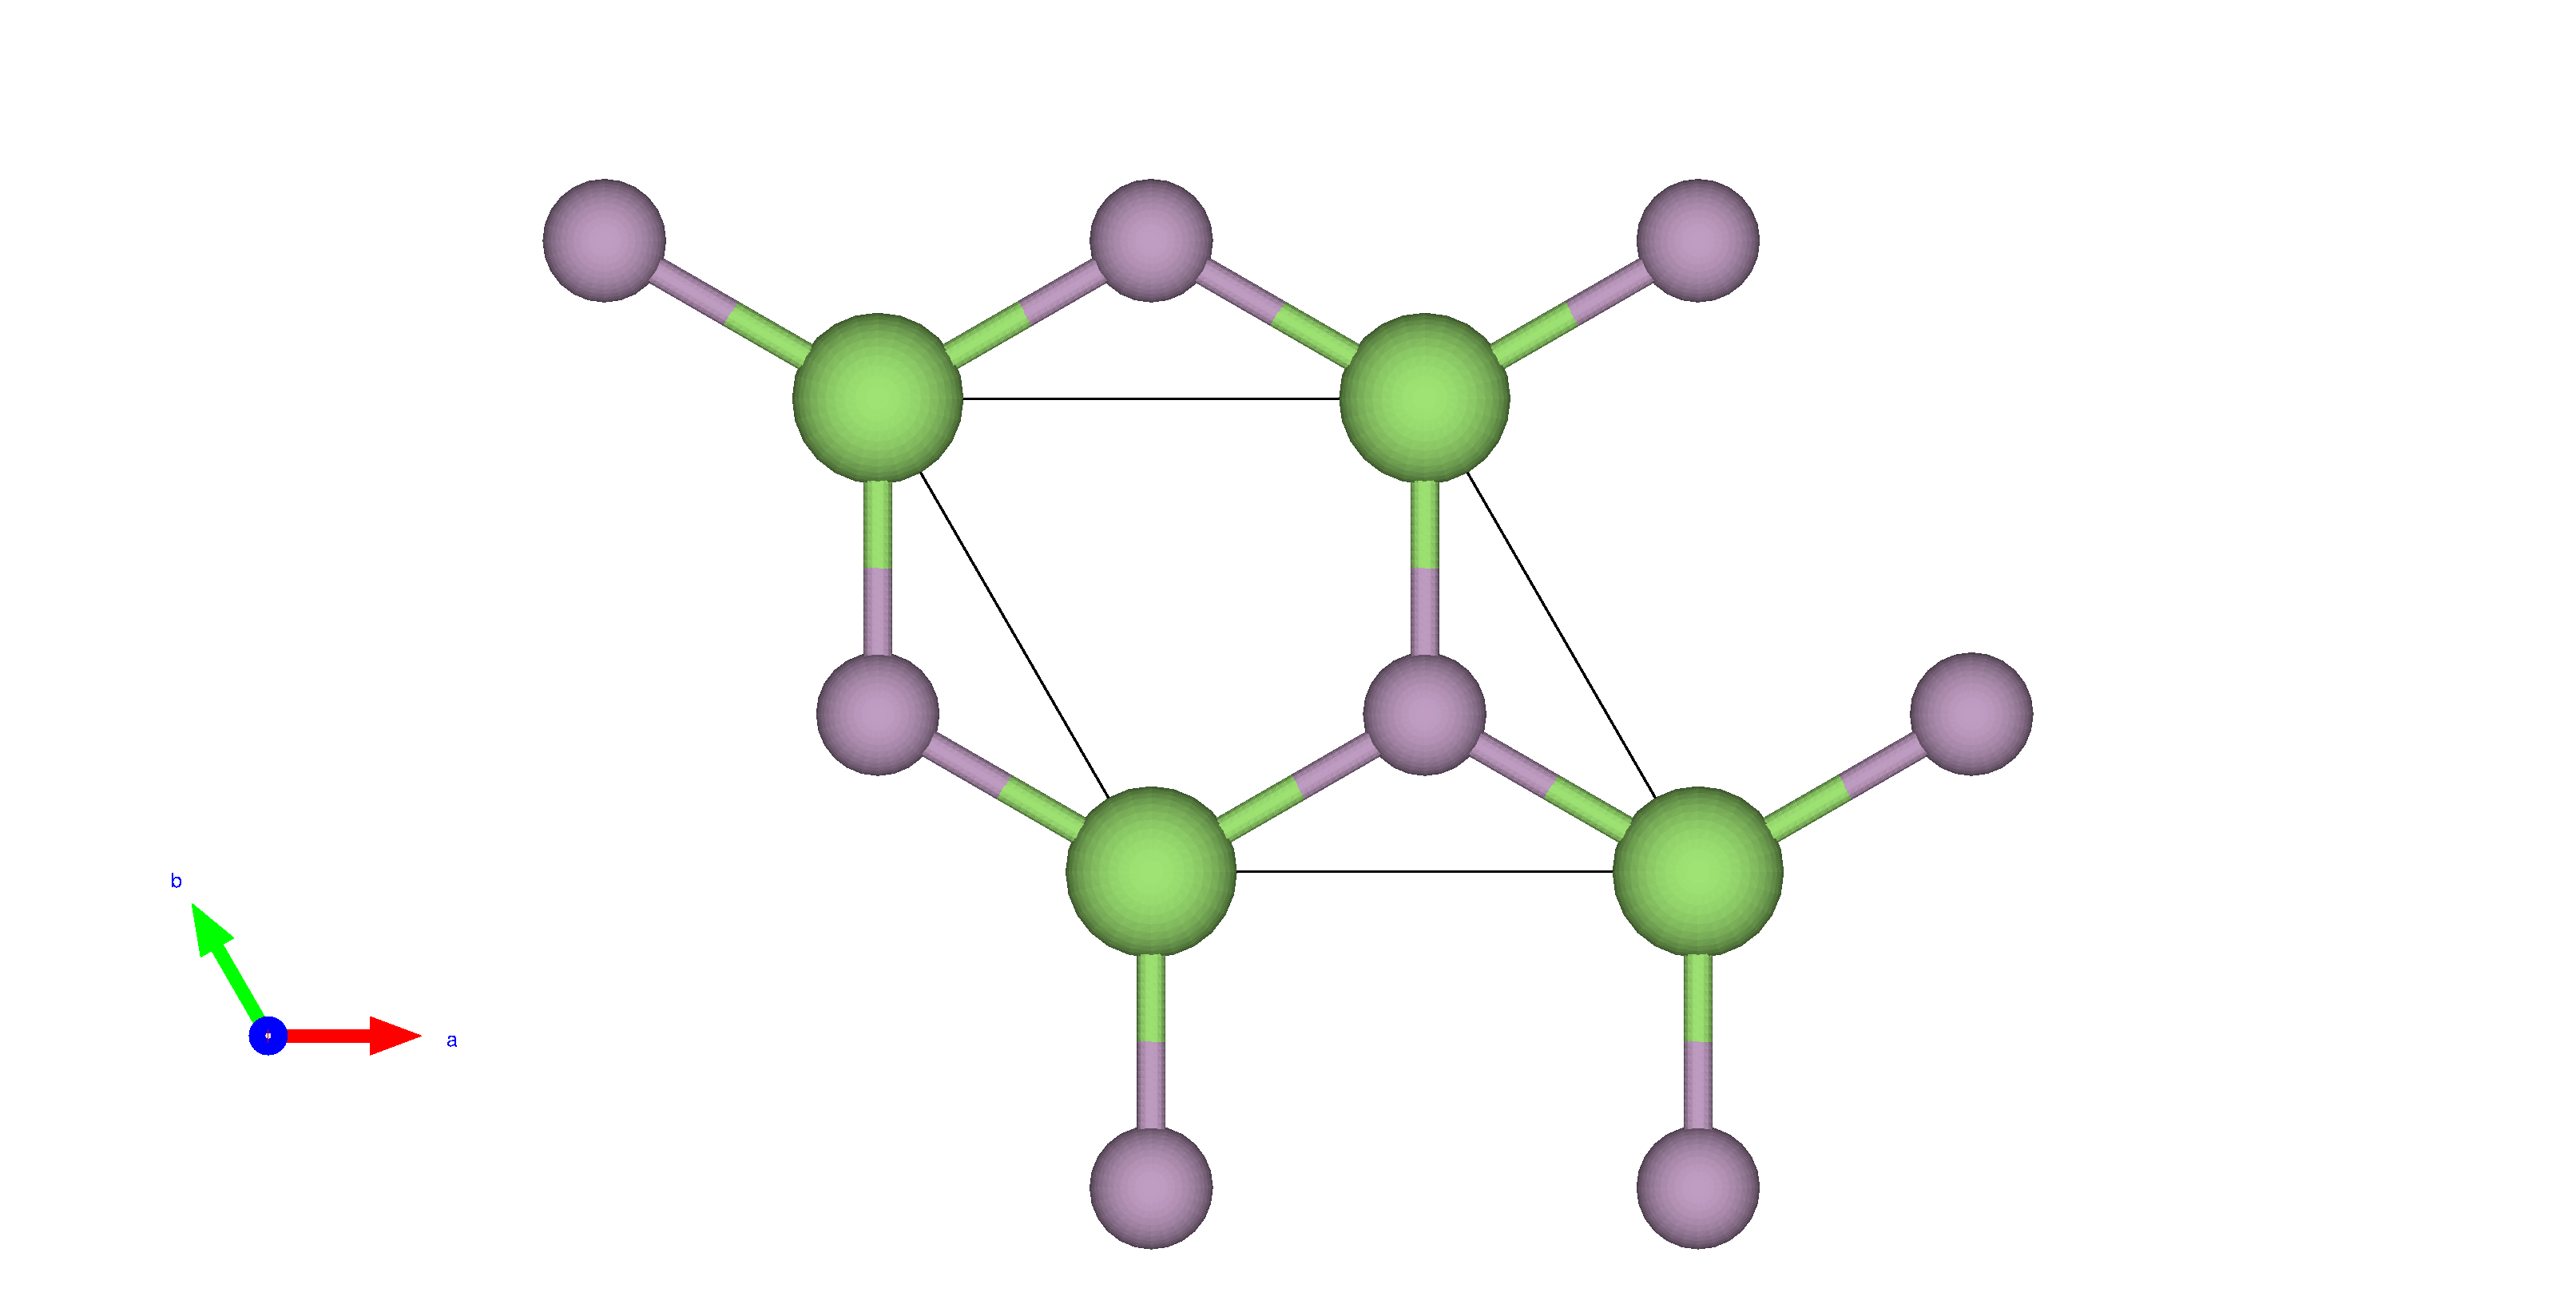
\includegraphics[width=\linewidth]{images/gap_st_2d.eps}
  \caption{GaP}
\end{subfigure}\hfil % <-- added
\begin{subfigure}{0.3\textwidth}
  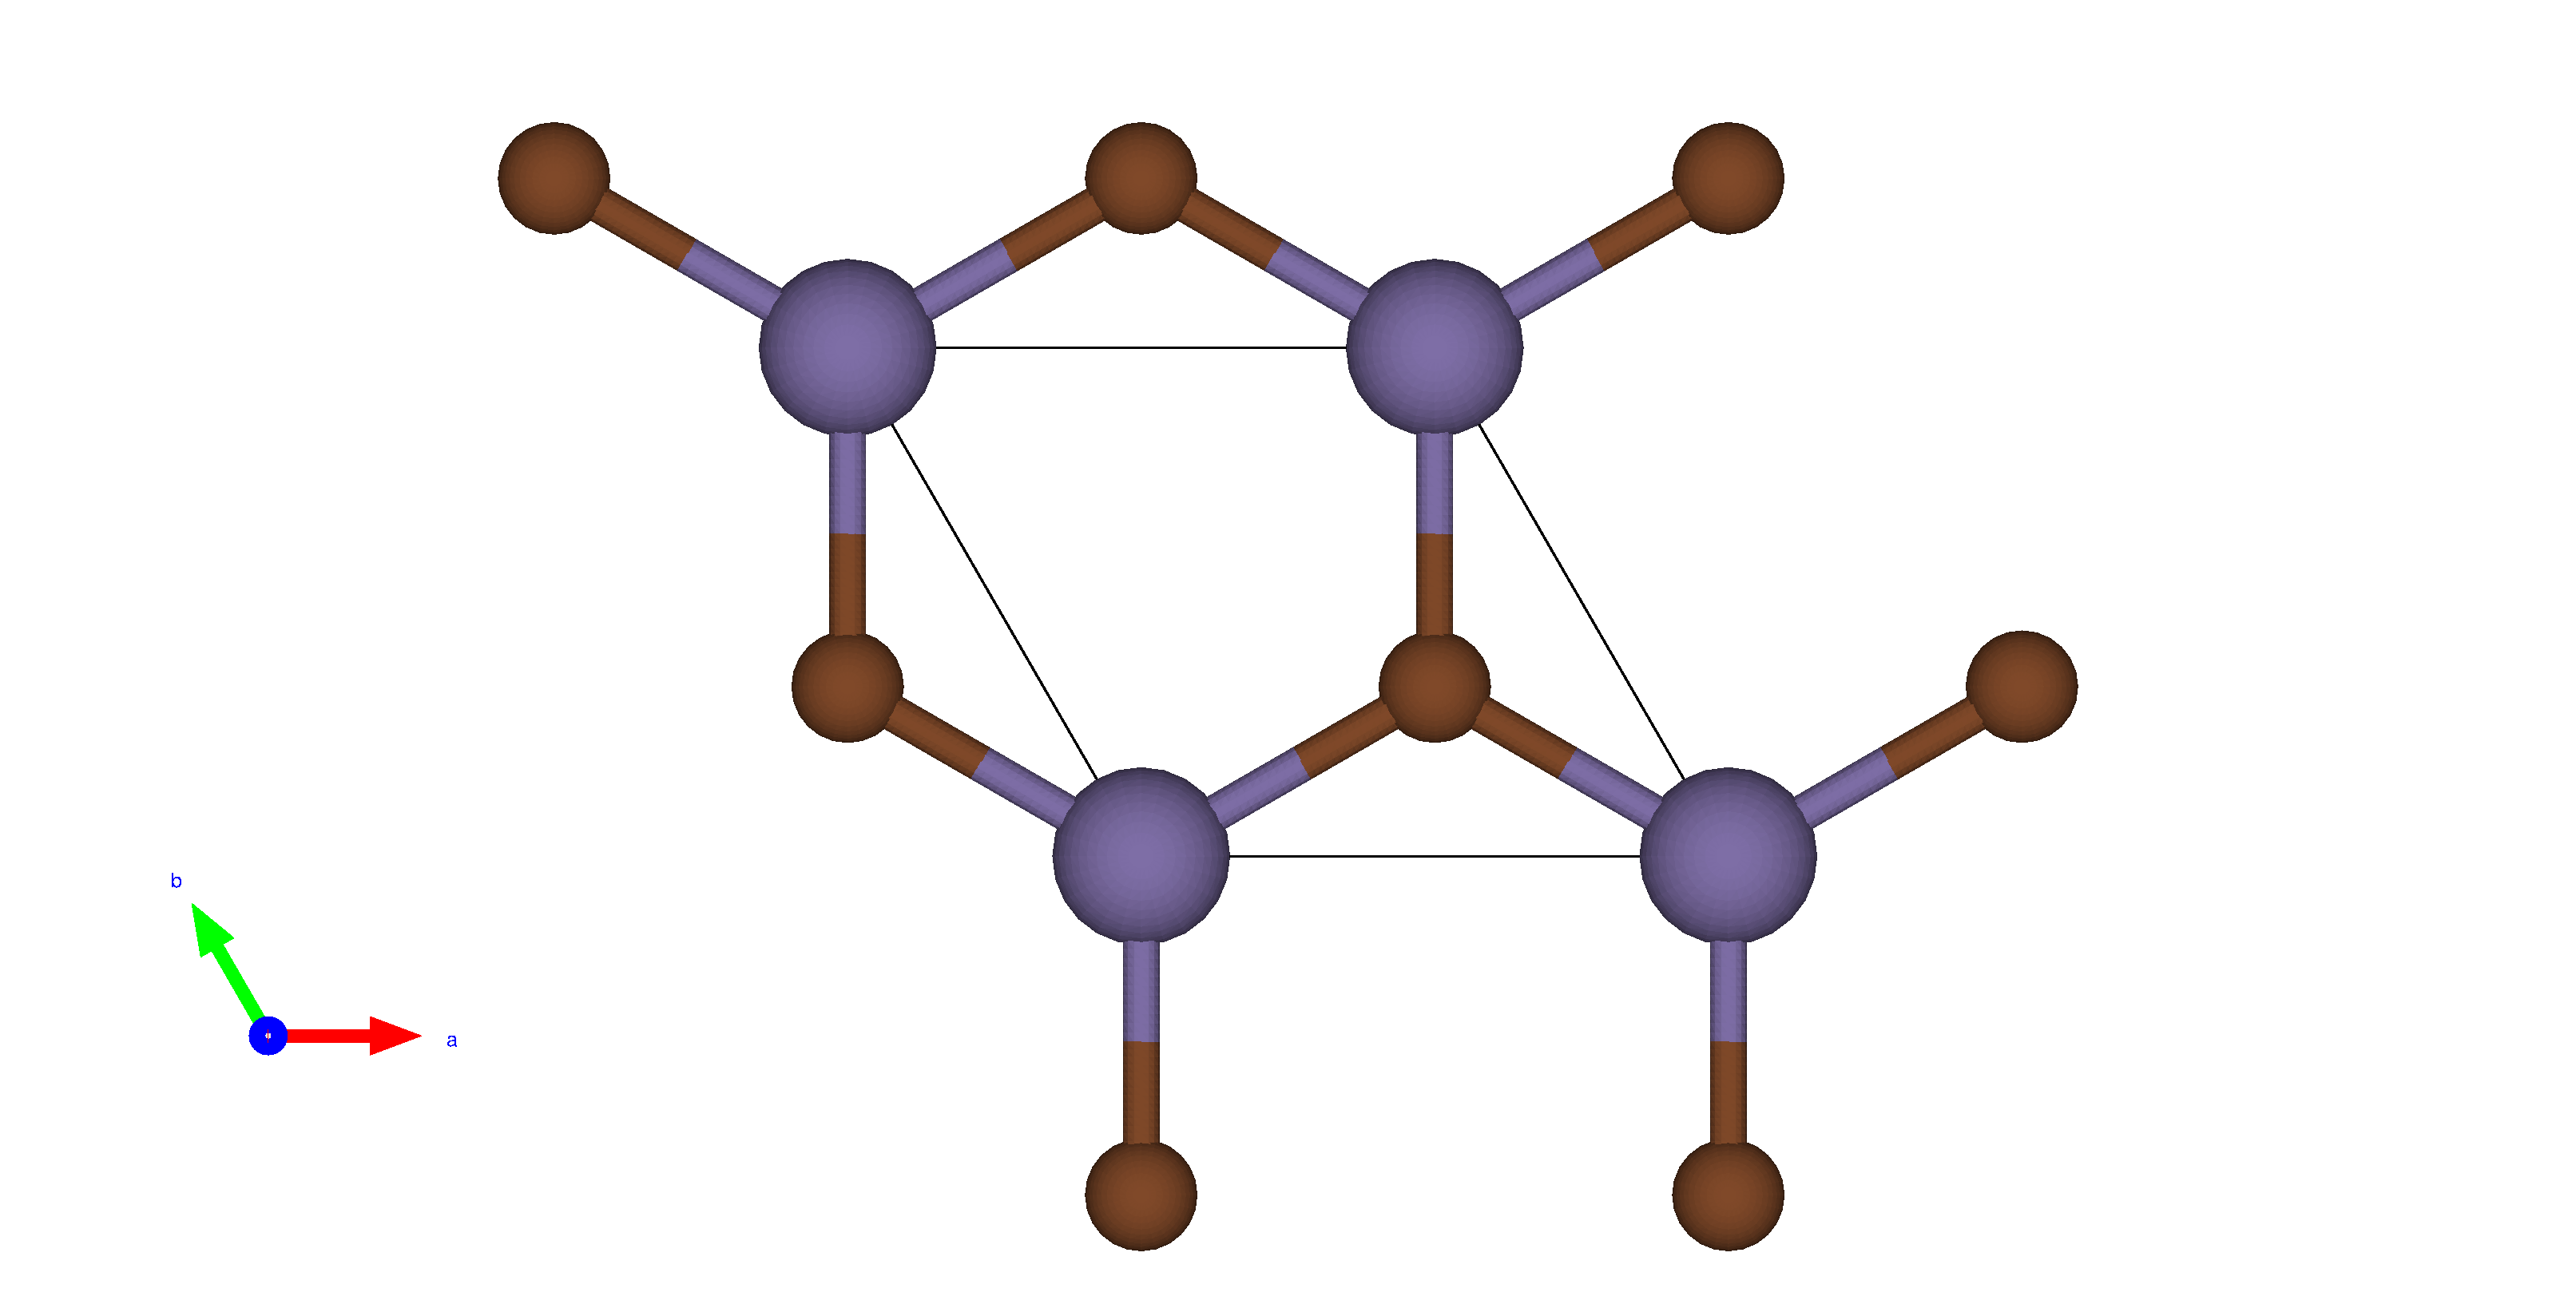
\includegraphics[width=\linewidth]{images/gec_st_2d.eps}
  \caption{GeC}
\end{subfigure}\hfil % <-- added
\begin{subfigure}{0.3\textwidth}
  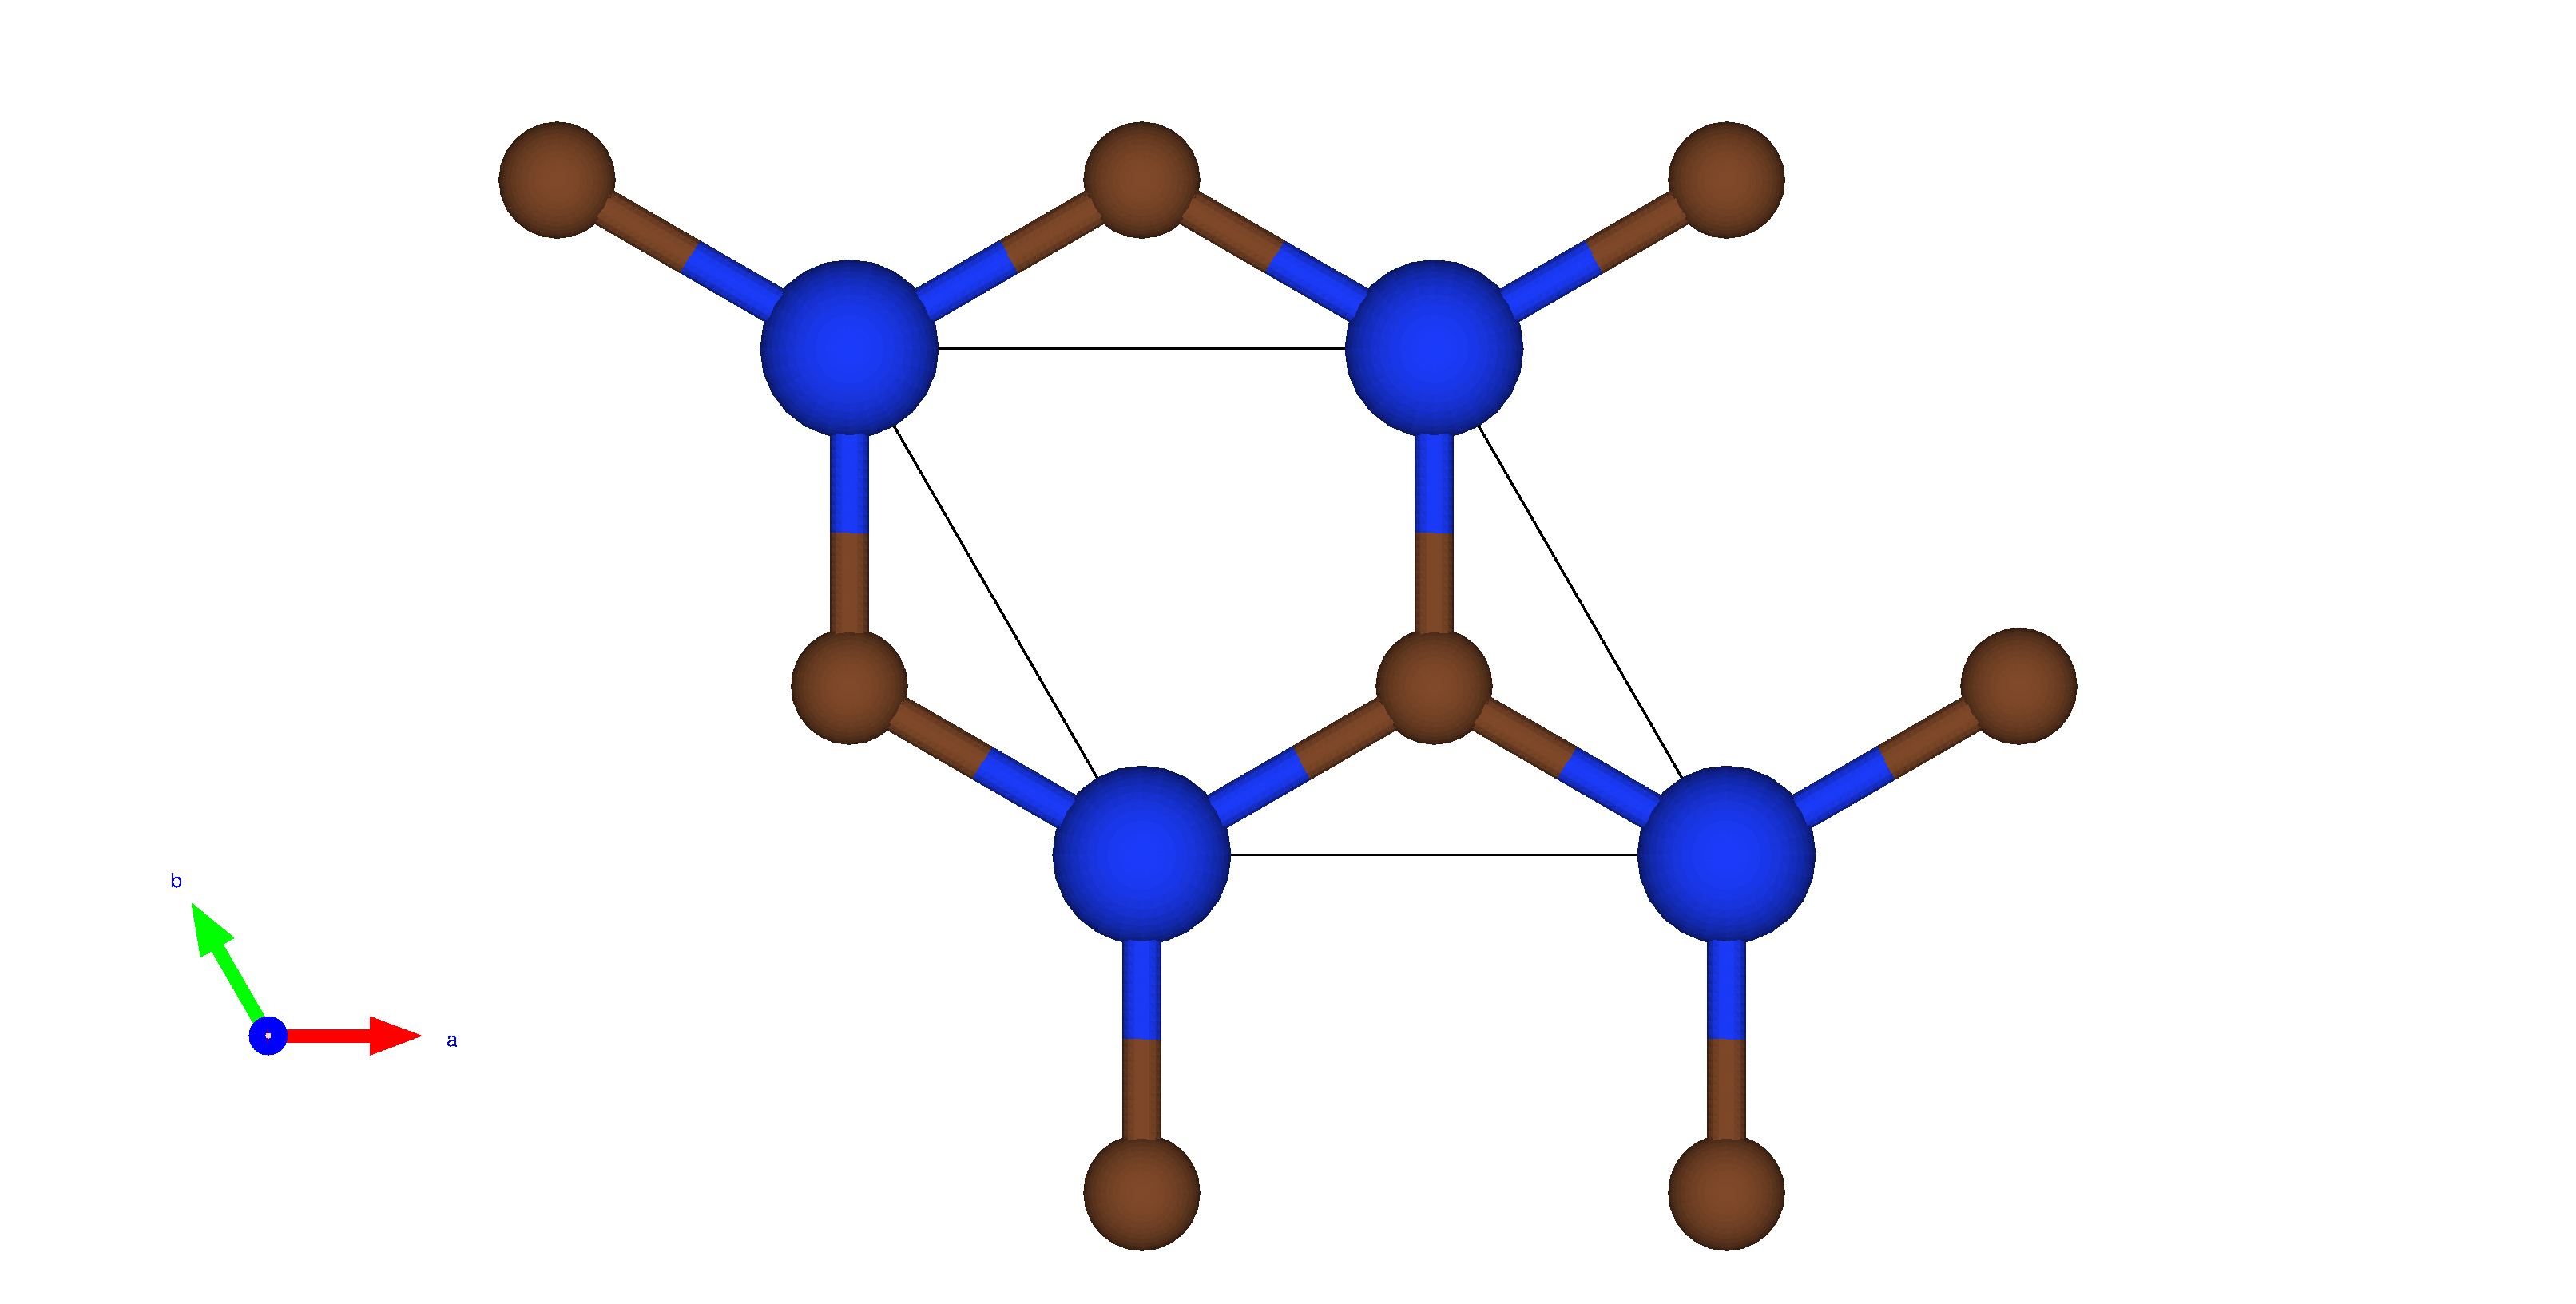
\includegraphics[width=\linewidth]{images/sic_st_2d.eps}
  \caption{SiC}
\end{subfigure}
\medskip
\begin{subfigure}{0.3\textwidth}
  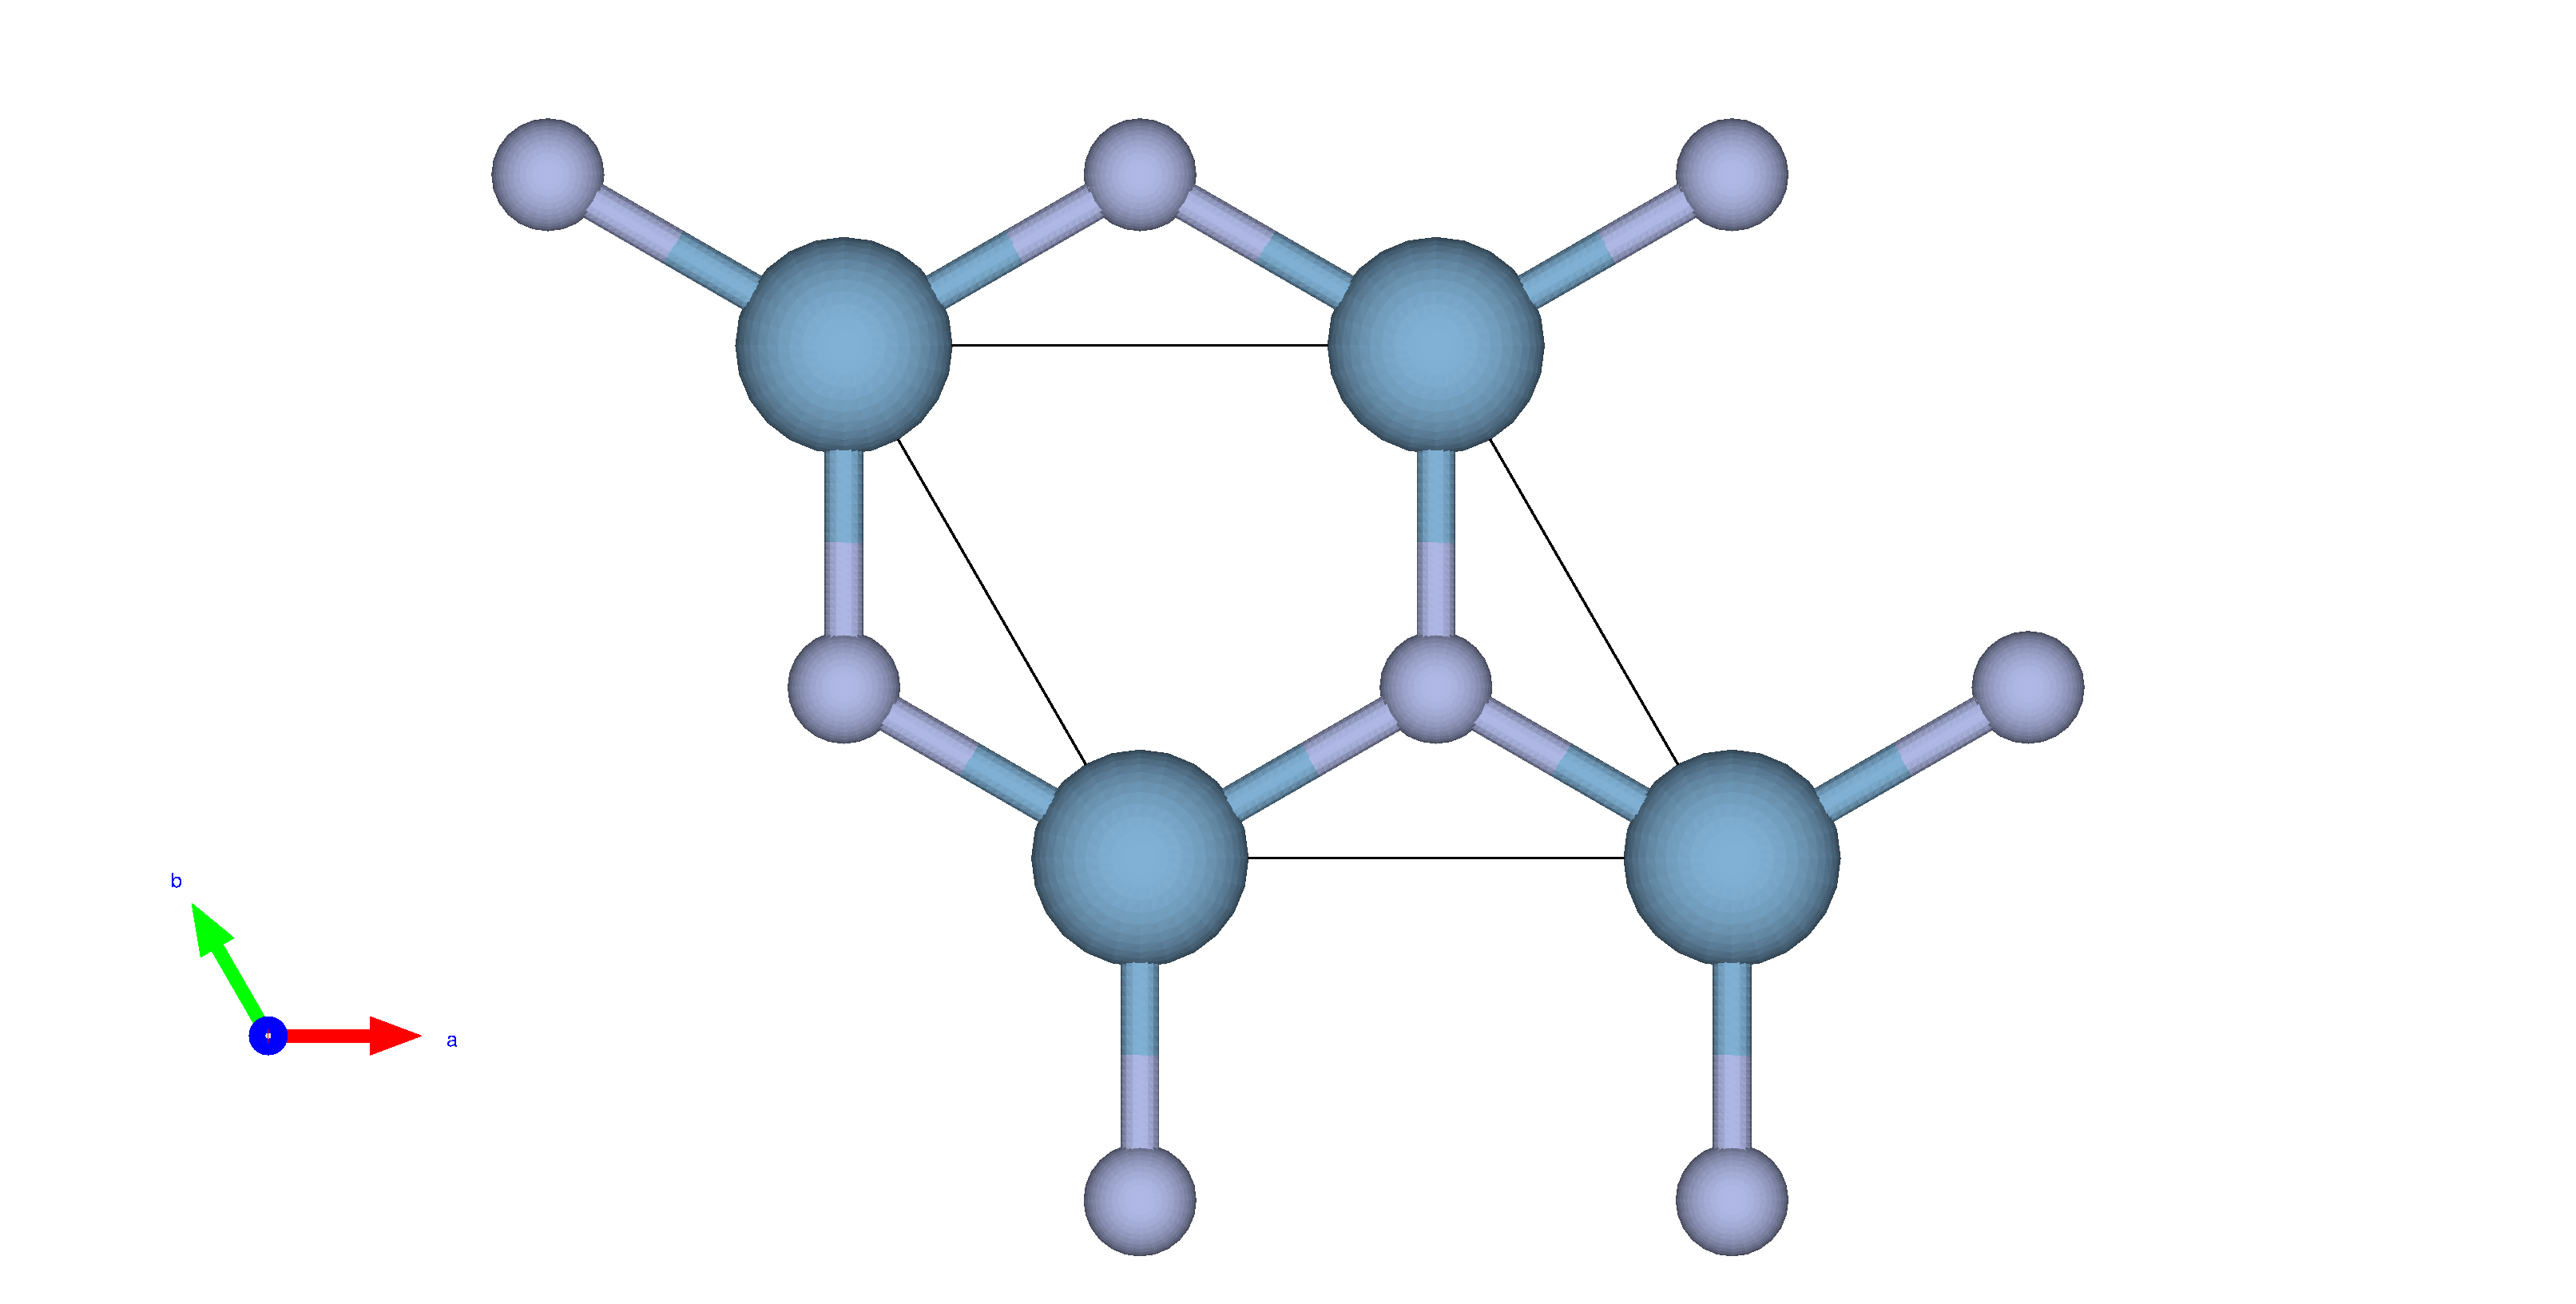
\includegraphics[width=\linewidth]{images/aln_st_2d.eps}
  \caption{AlN}
\end{subfigure}

\caption{Structures of all 2D materials used in this study.}
\label{fig:2d_materials_structure}

\end{figure}

\begin{figure}[htb]
    \centering % <-- added
\begin{subfigure}{0.3\textwidth}
  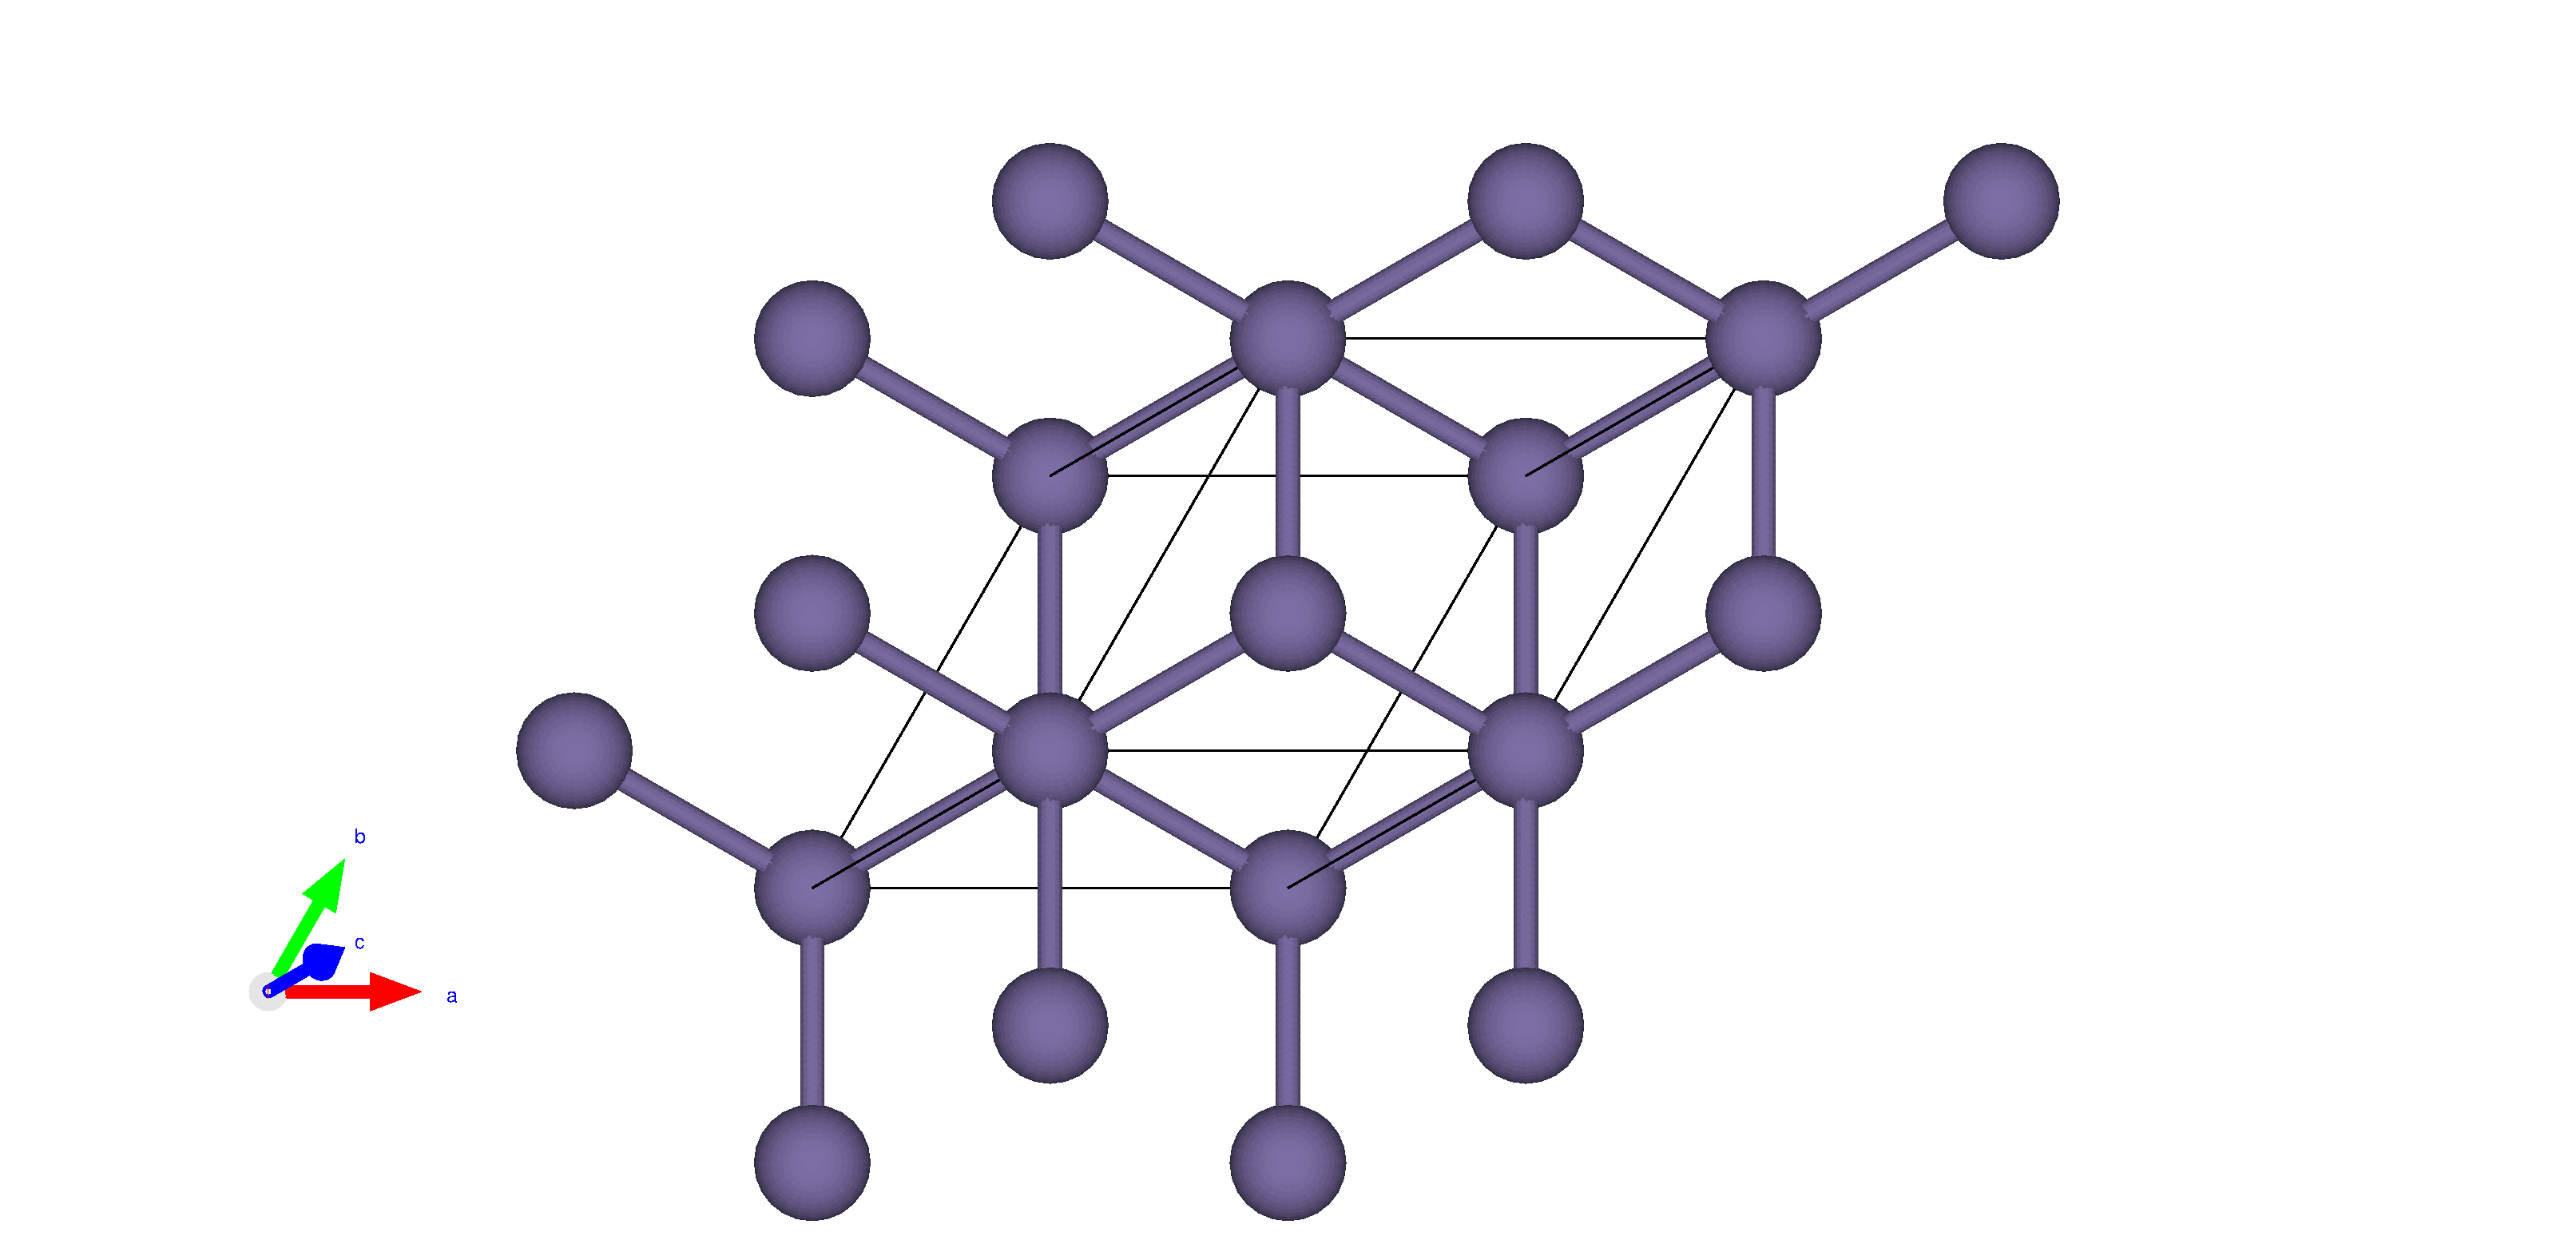
\includegraphics[width=\linewidth]{images/ge_st_3d.eps}
  \caption{Ge}
\end{subfigure}\hfil % <-- added
\begin{subfigure}{0.3\textwidth}
  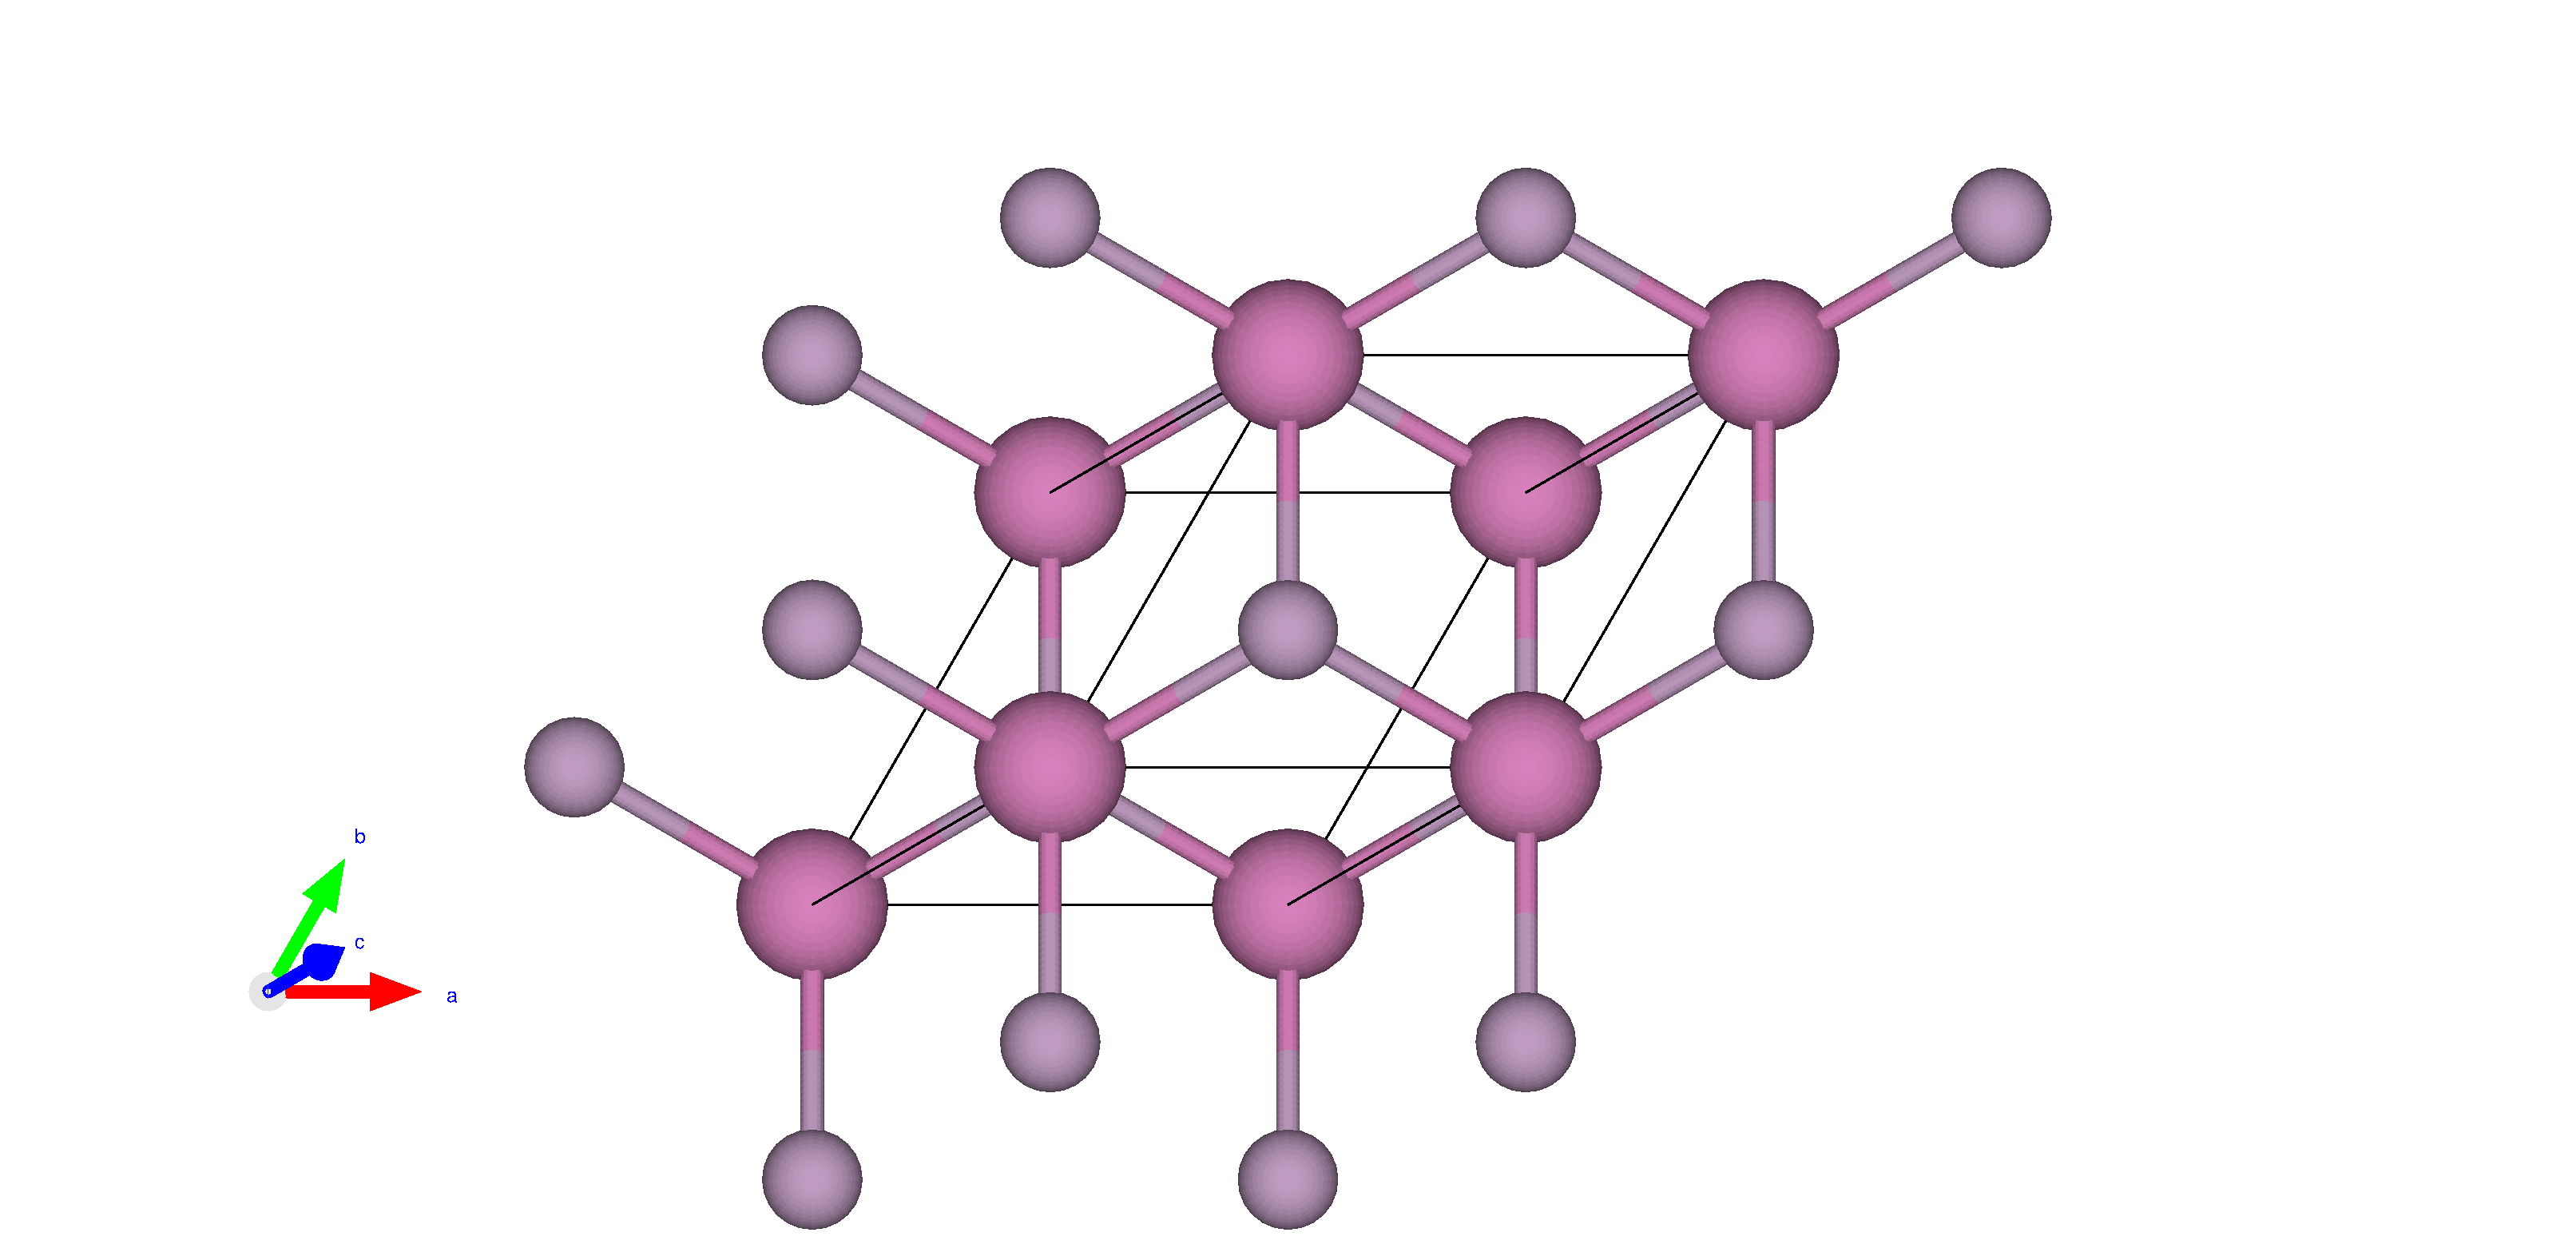
\includegraphics[width=\linewidth]{images/inp_st_3d.eps}
  \caption{InP}
\end{subfigure}
\begin{subfigure}{0.3\textwidth}
  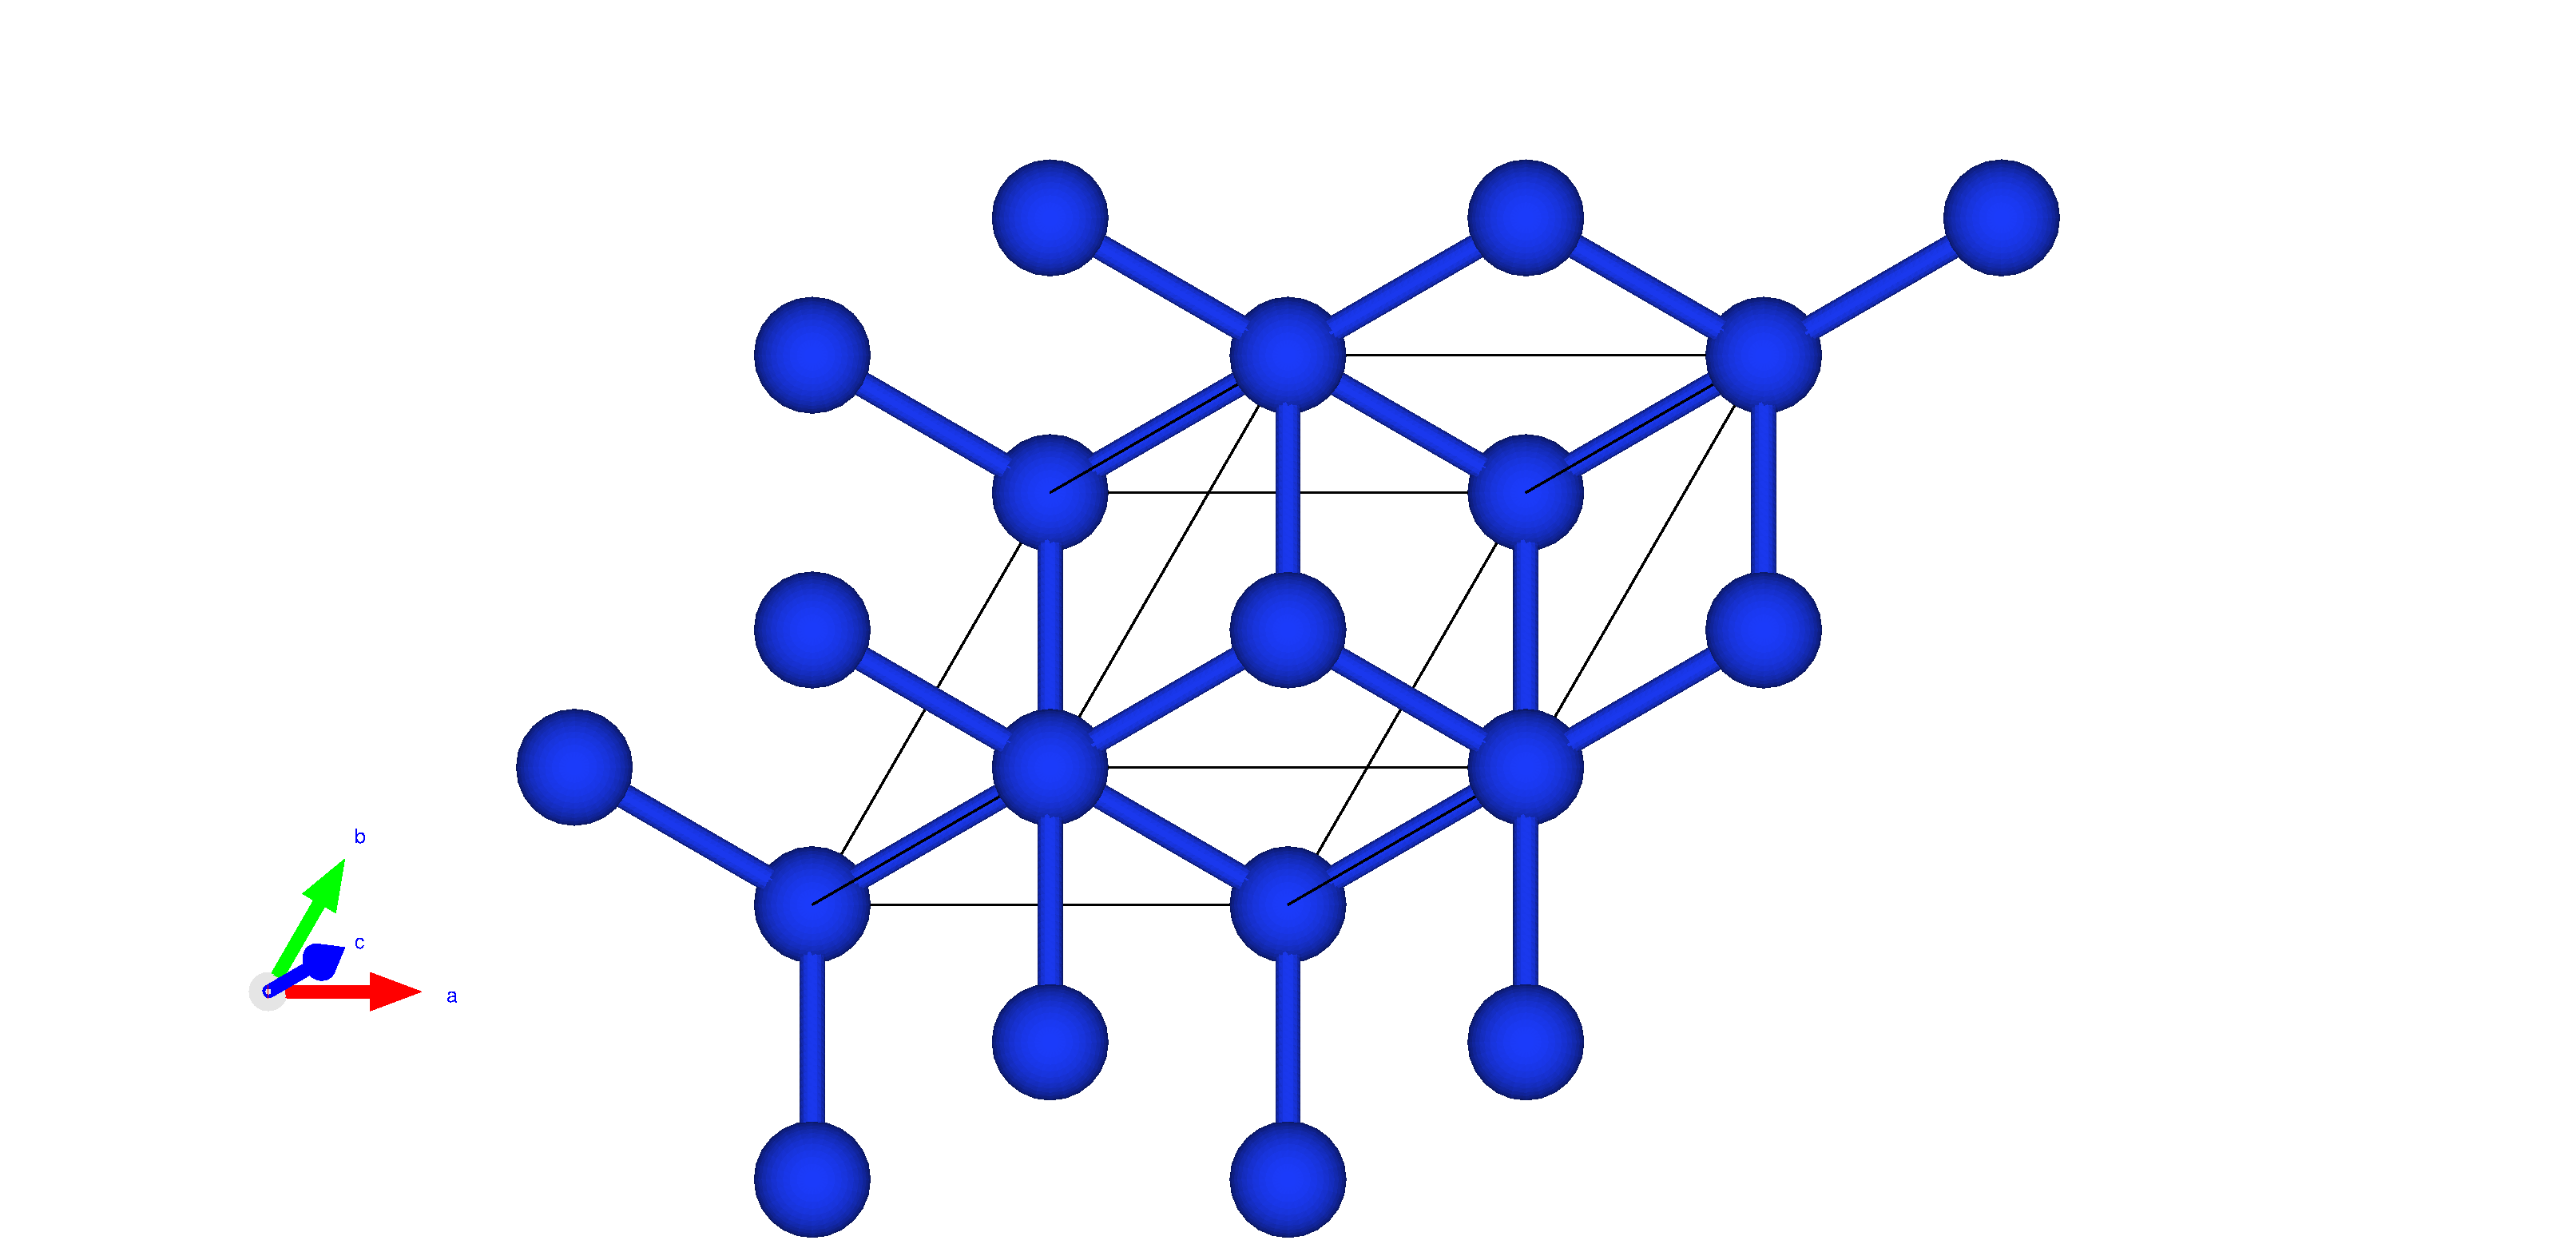
\includegraphics[width=\linewidth]{images/si_st_3d.eps}
  \caption{Si}
\end{subfigure}\hfil % <-- added

\medskip
\begin{subfigure}{0.3\textwidth}
  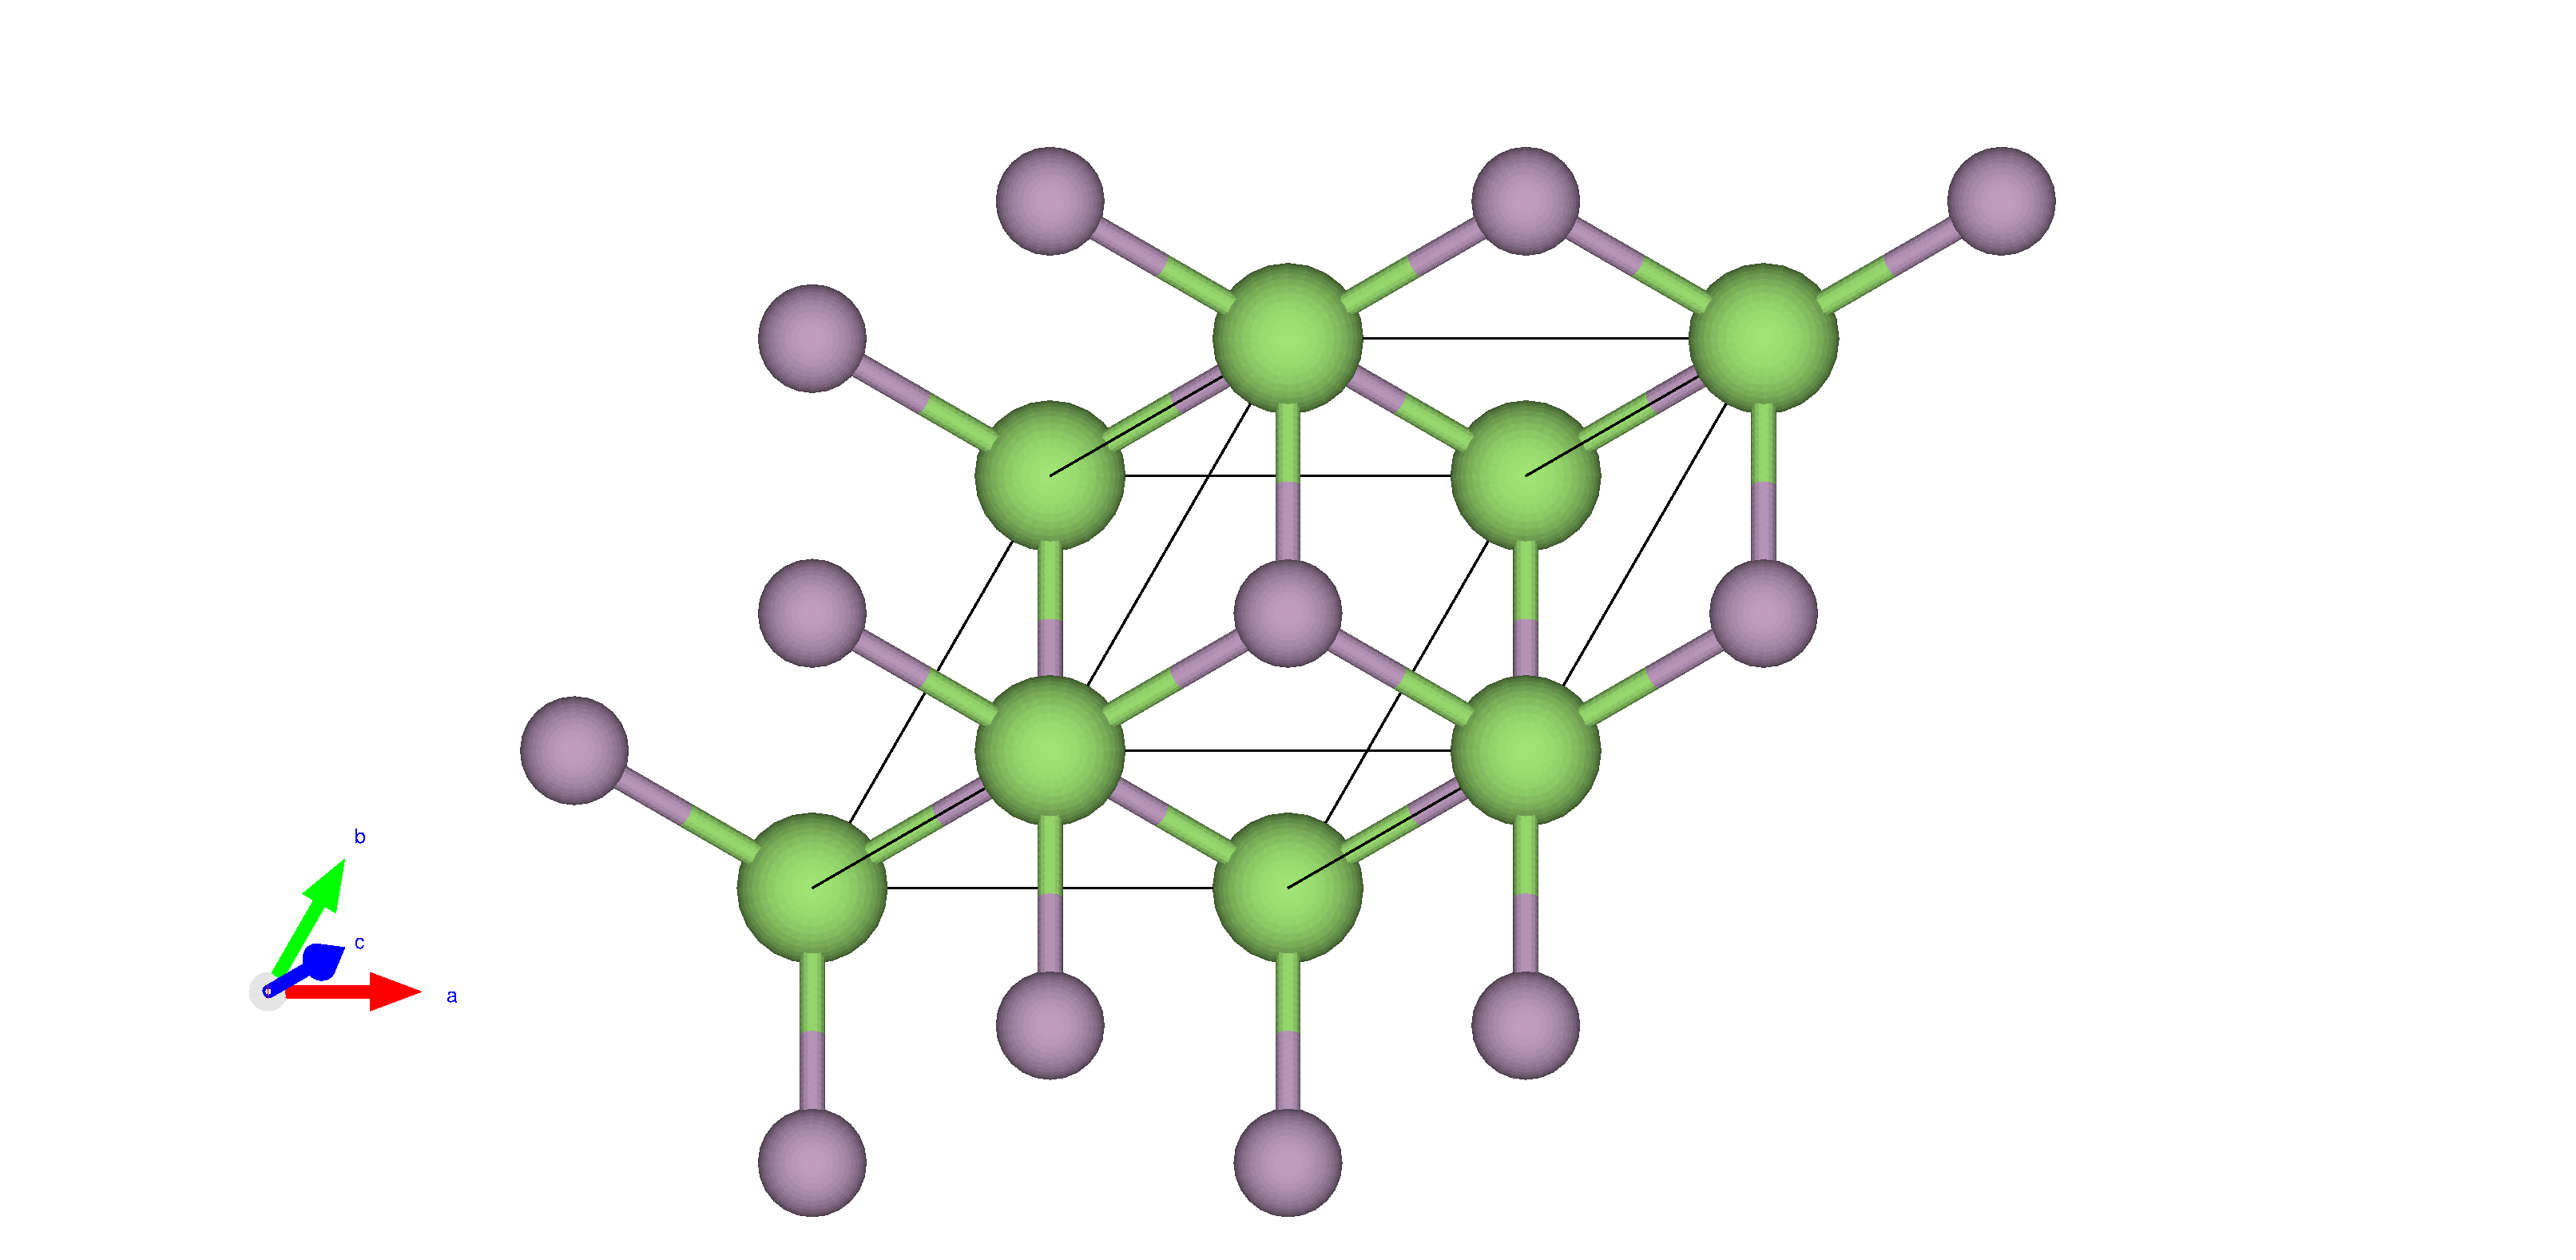
\includegraphics[width=\linewidth]{images/gap_st_3d.eps}
  \caption{GaP}
\end{subfigure}\hfil % <-- added
\begin{subfigure}{0.3\textwidth}
  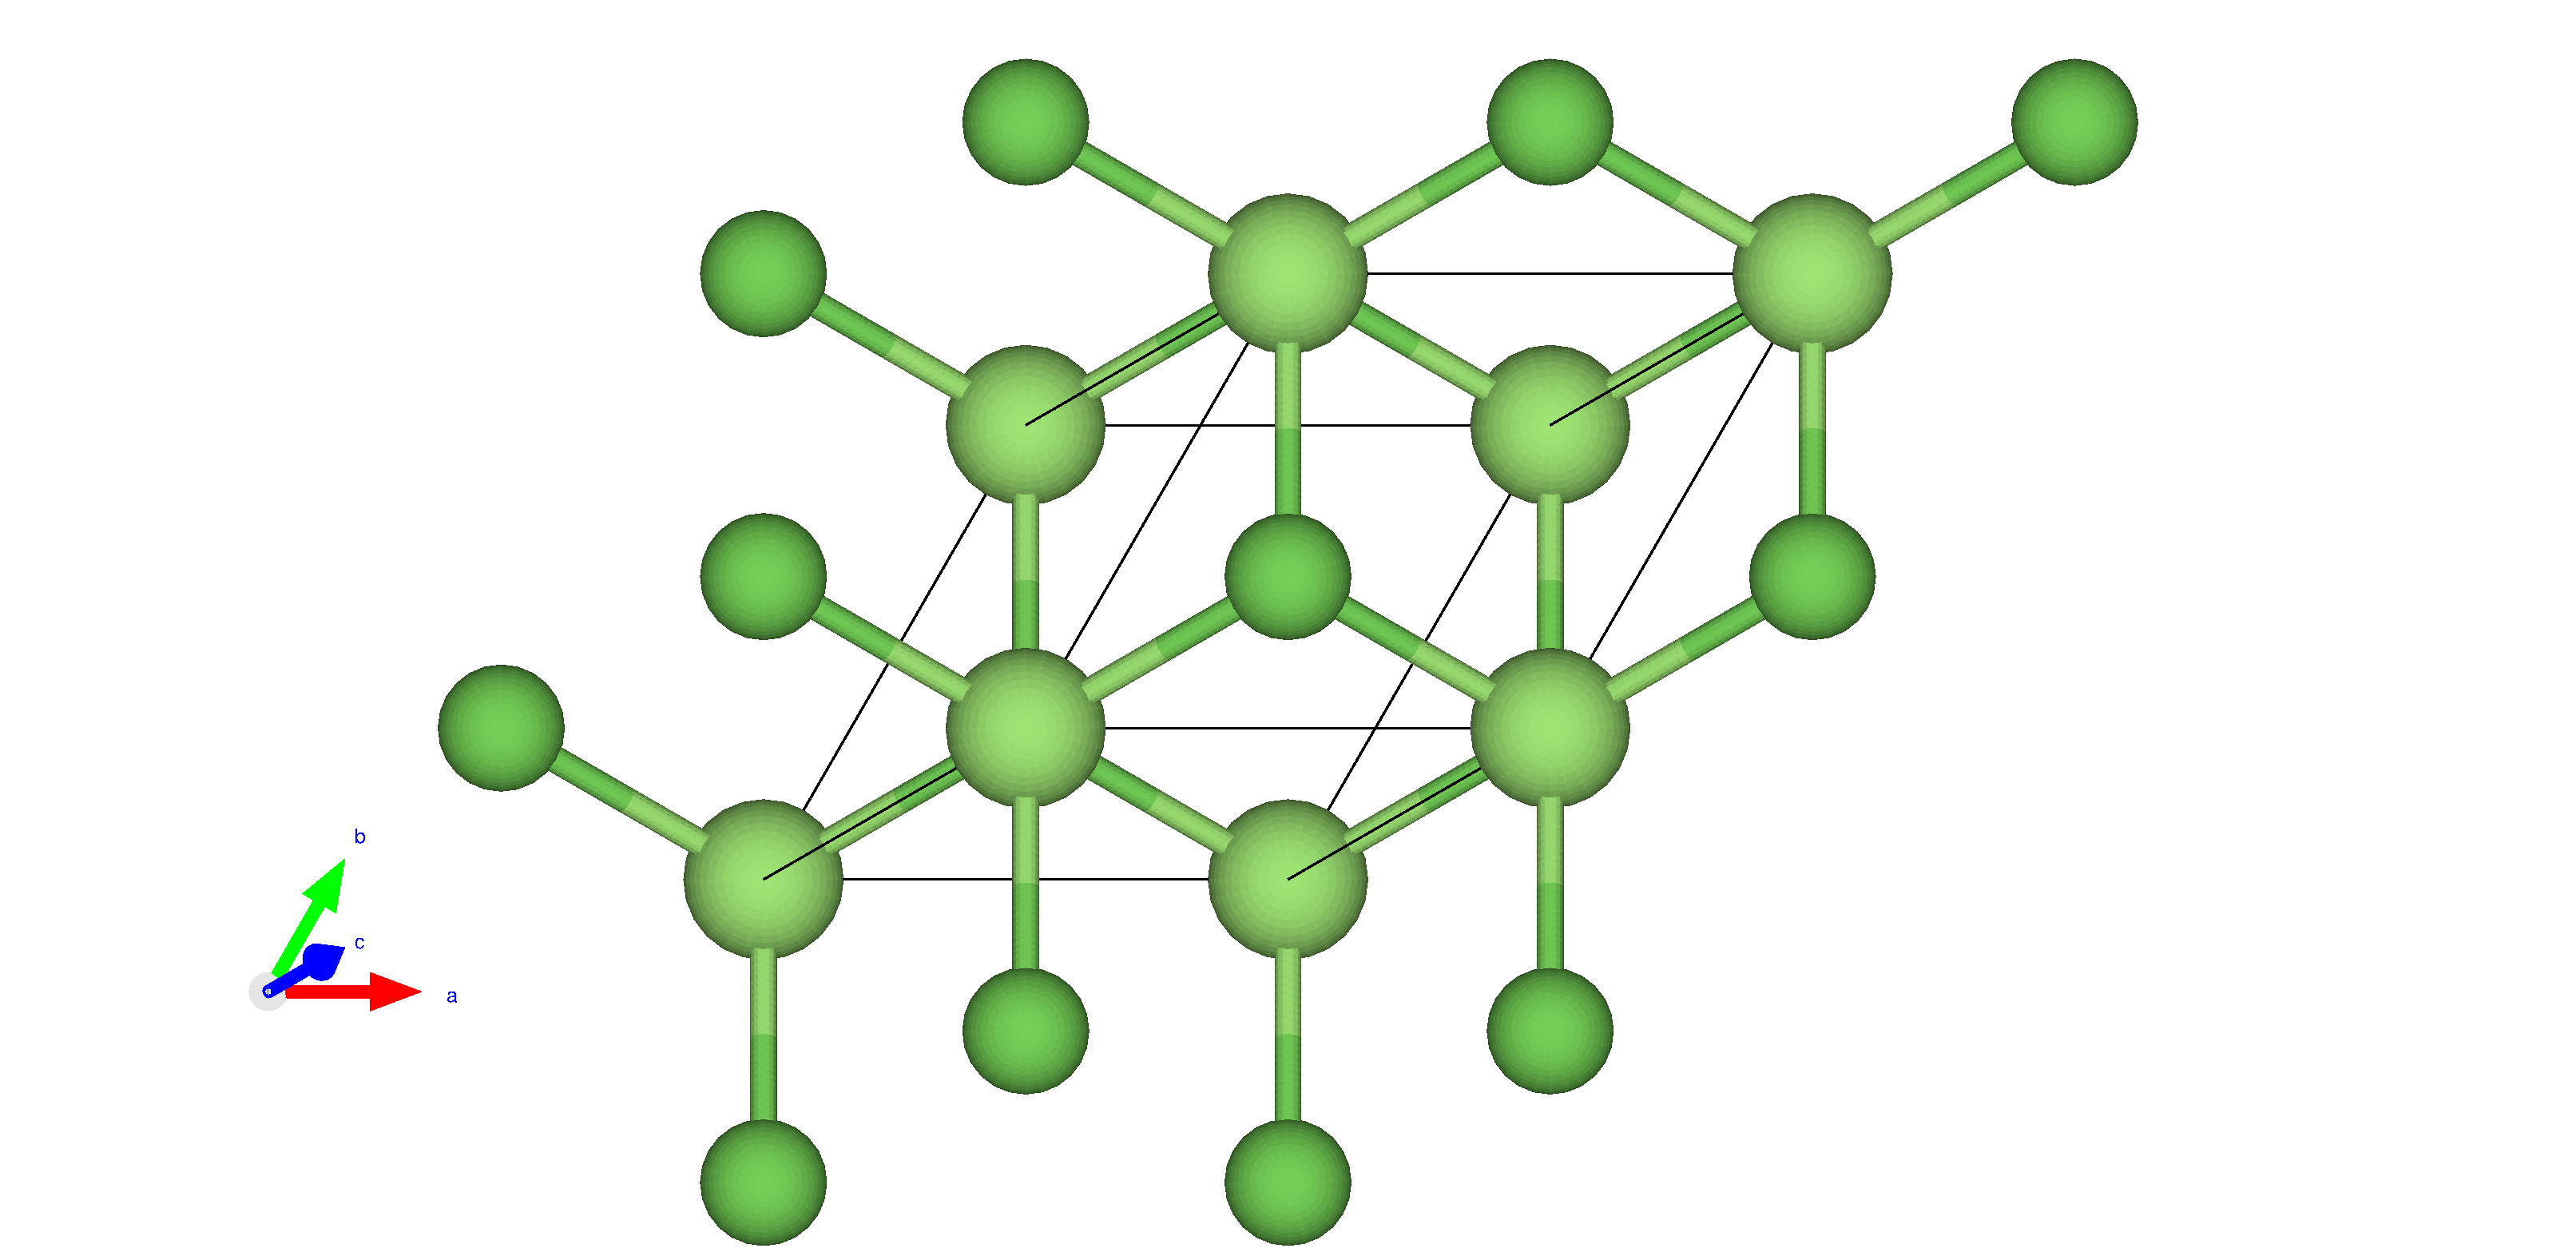
\includegraphics[width=\linewidth]{images/gaas_st_3d.eps}
  \caption{GaAs}
\end{subfigure}\hfil % <-- added
\begin{subfigure}{0.3\textwidth}
  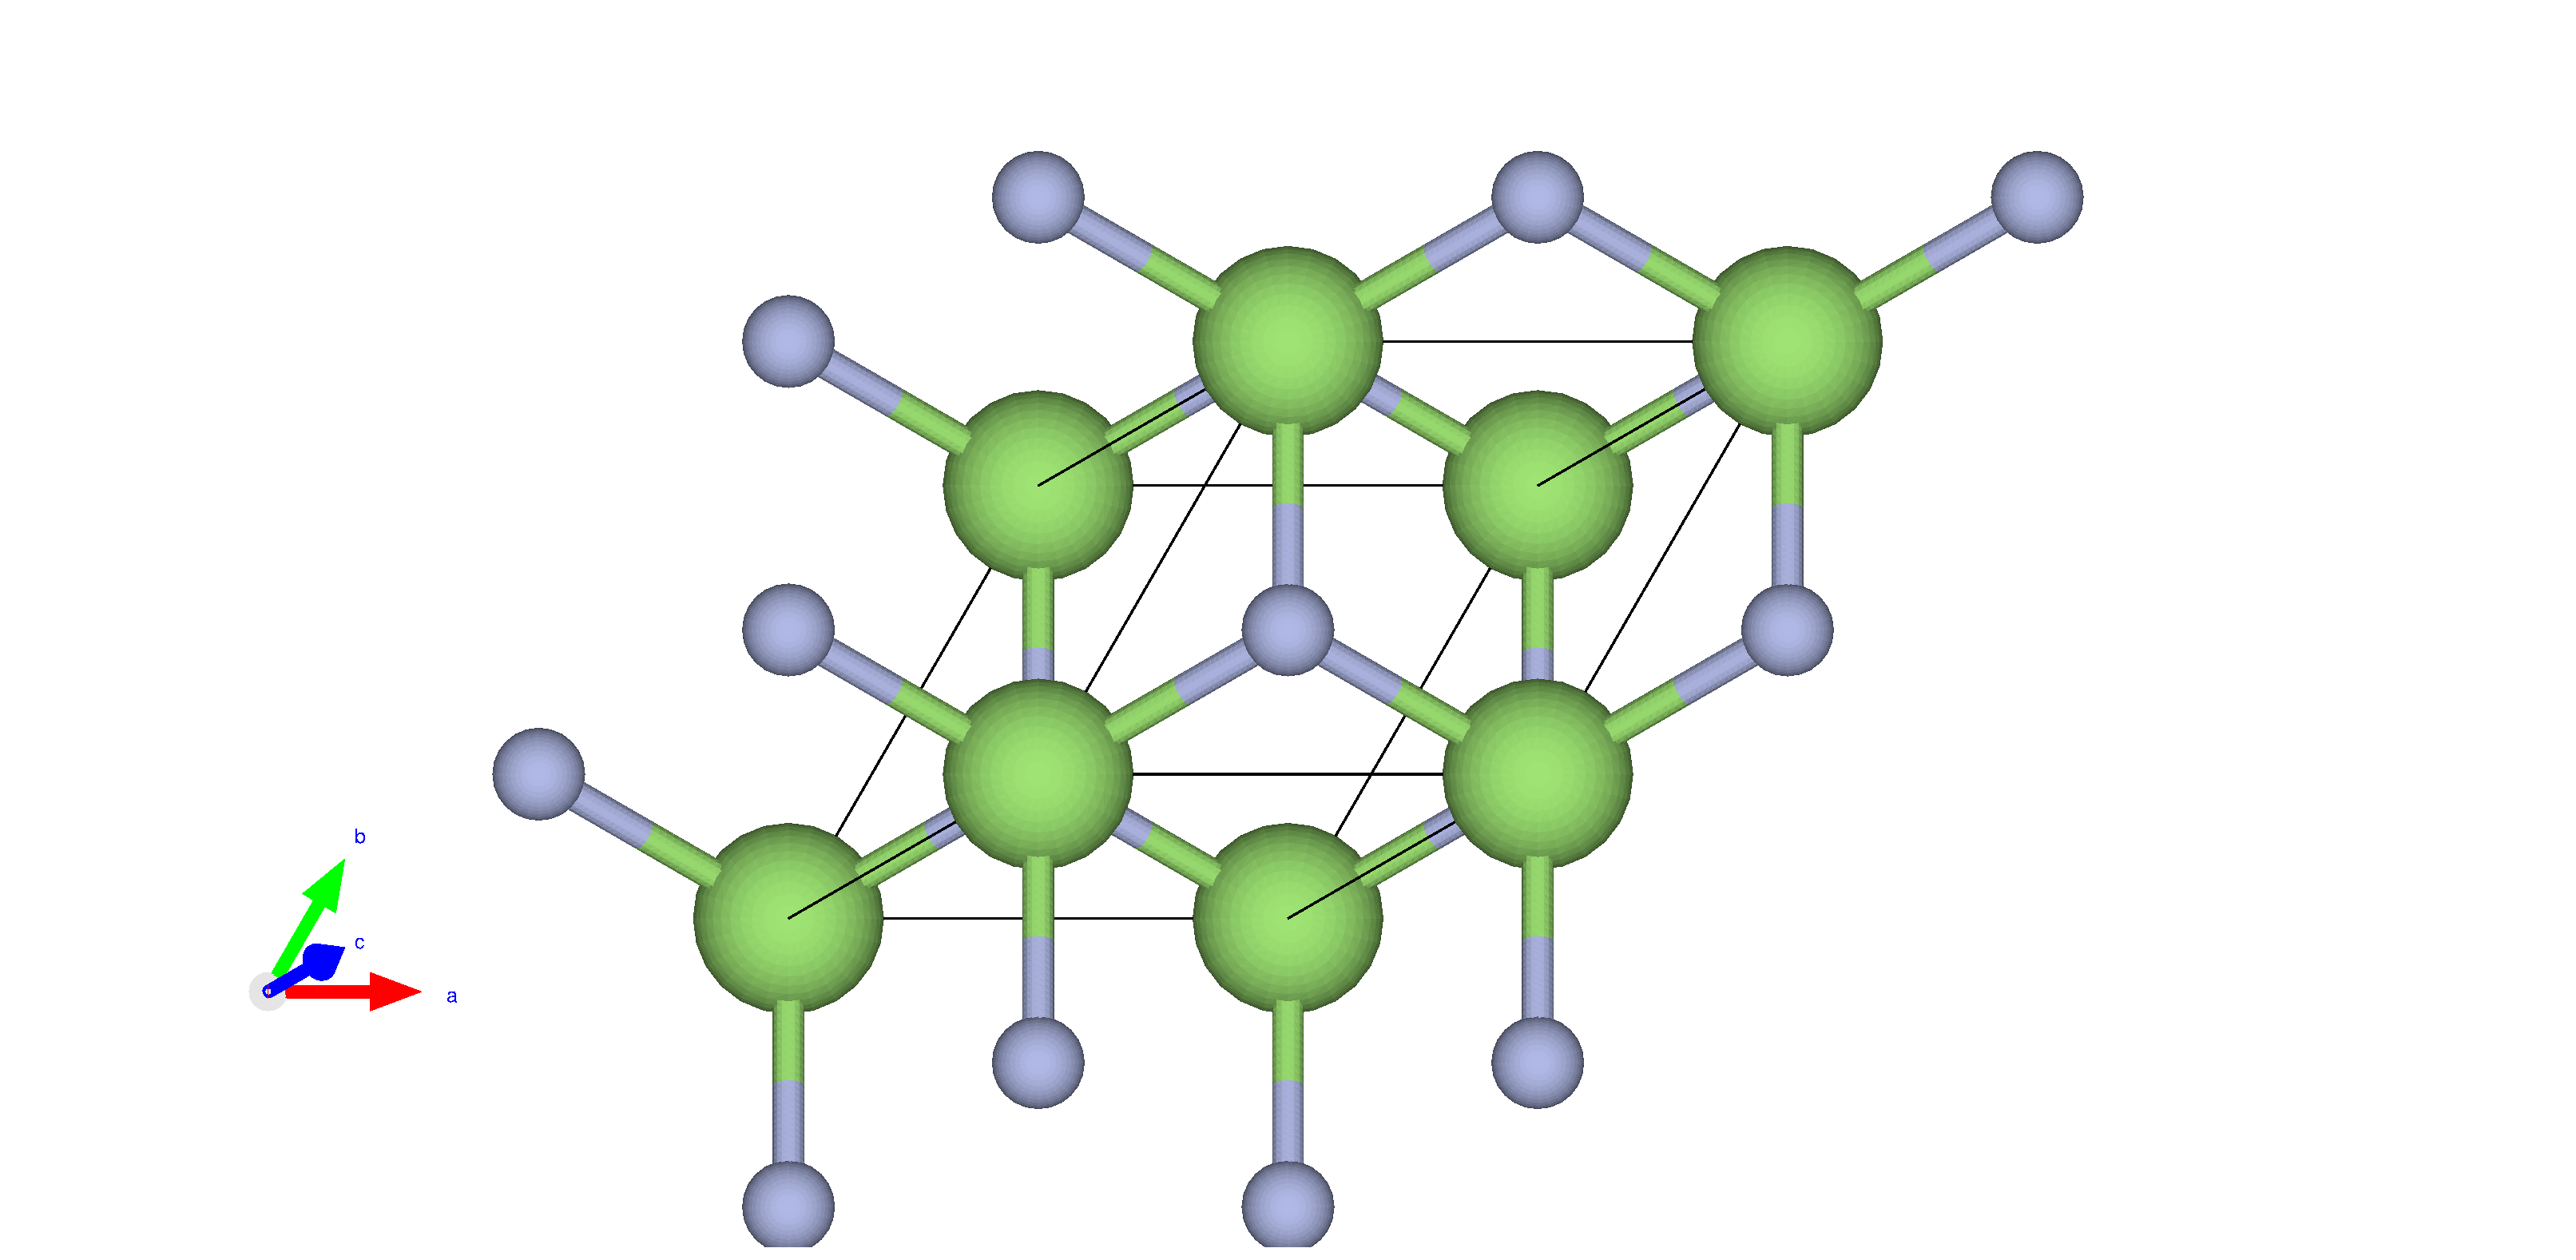
\includegraphics[width=\linewidth]{images/gan_st_3d.eps}
  \caption{GaN}
\end{subfigure}
\medskip
\begin{subfigure}{0.3\textwidth}
  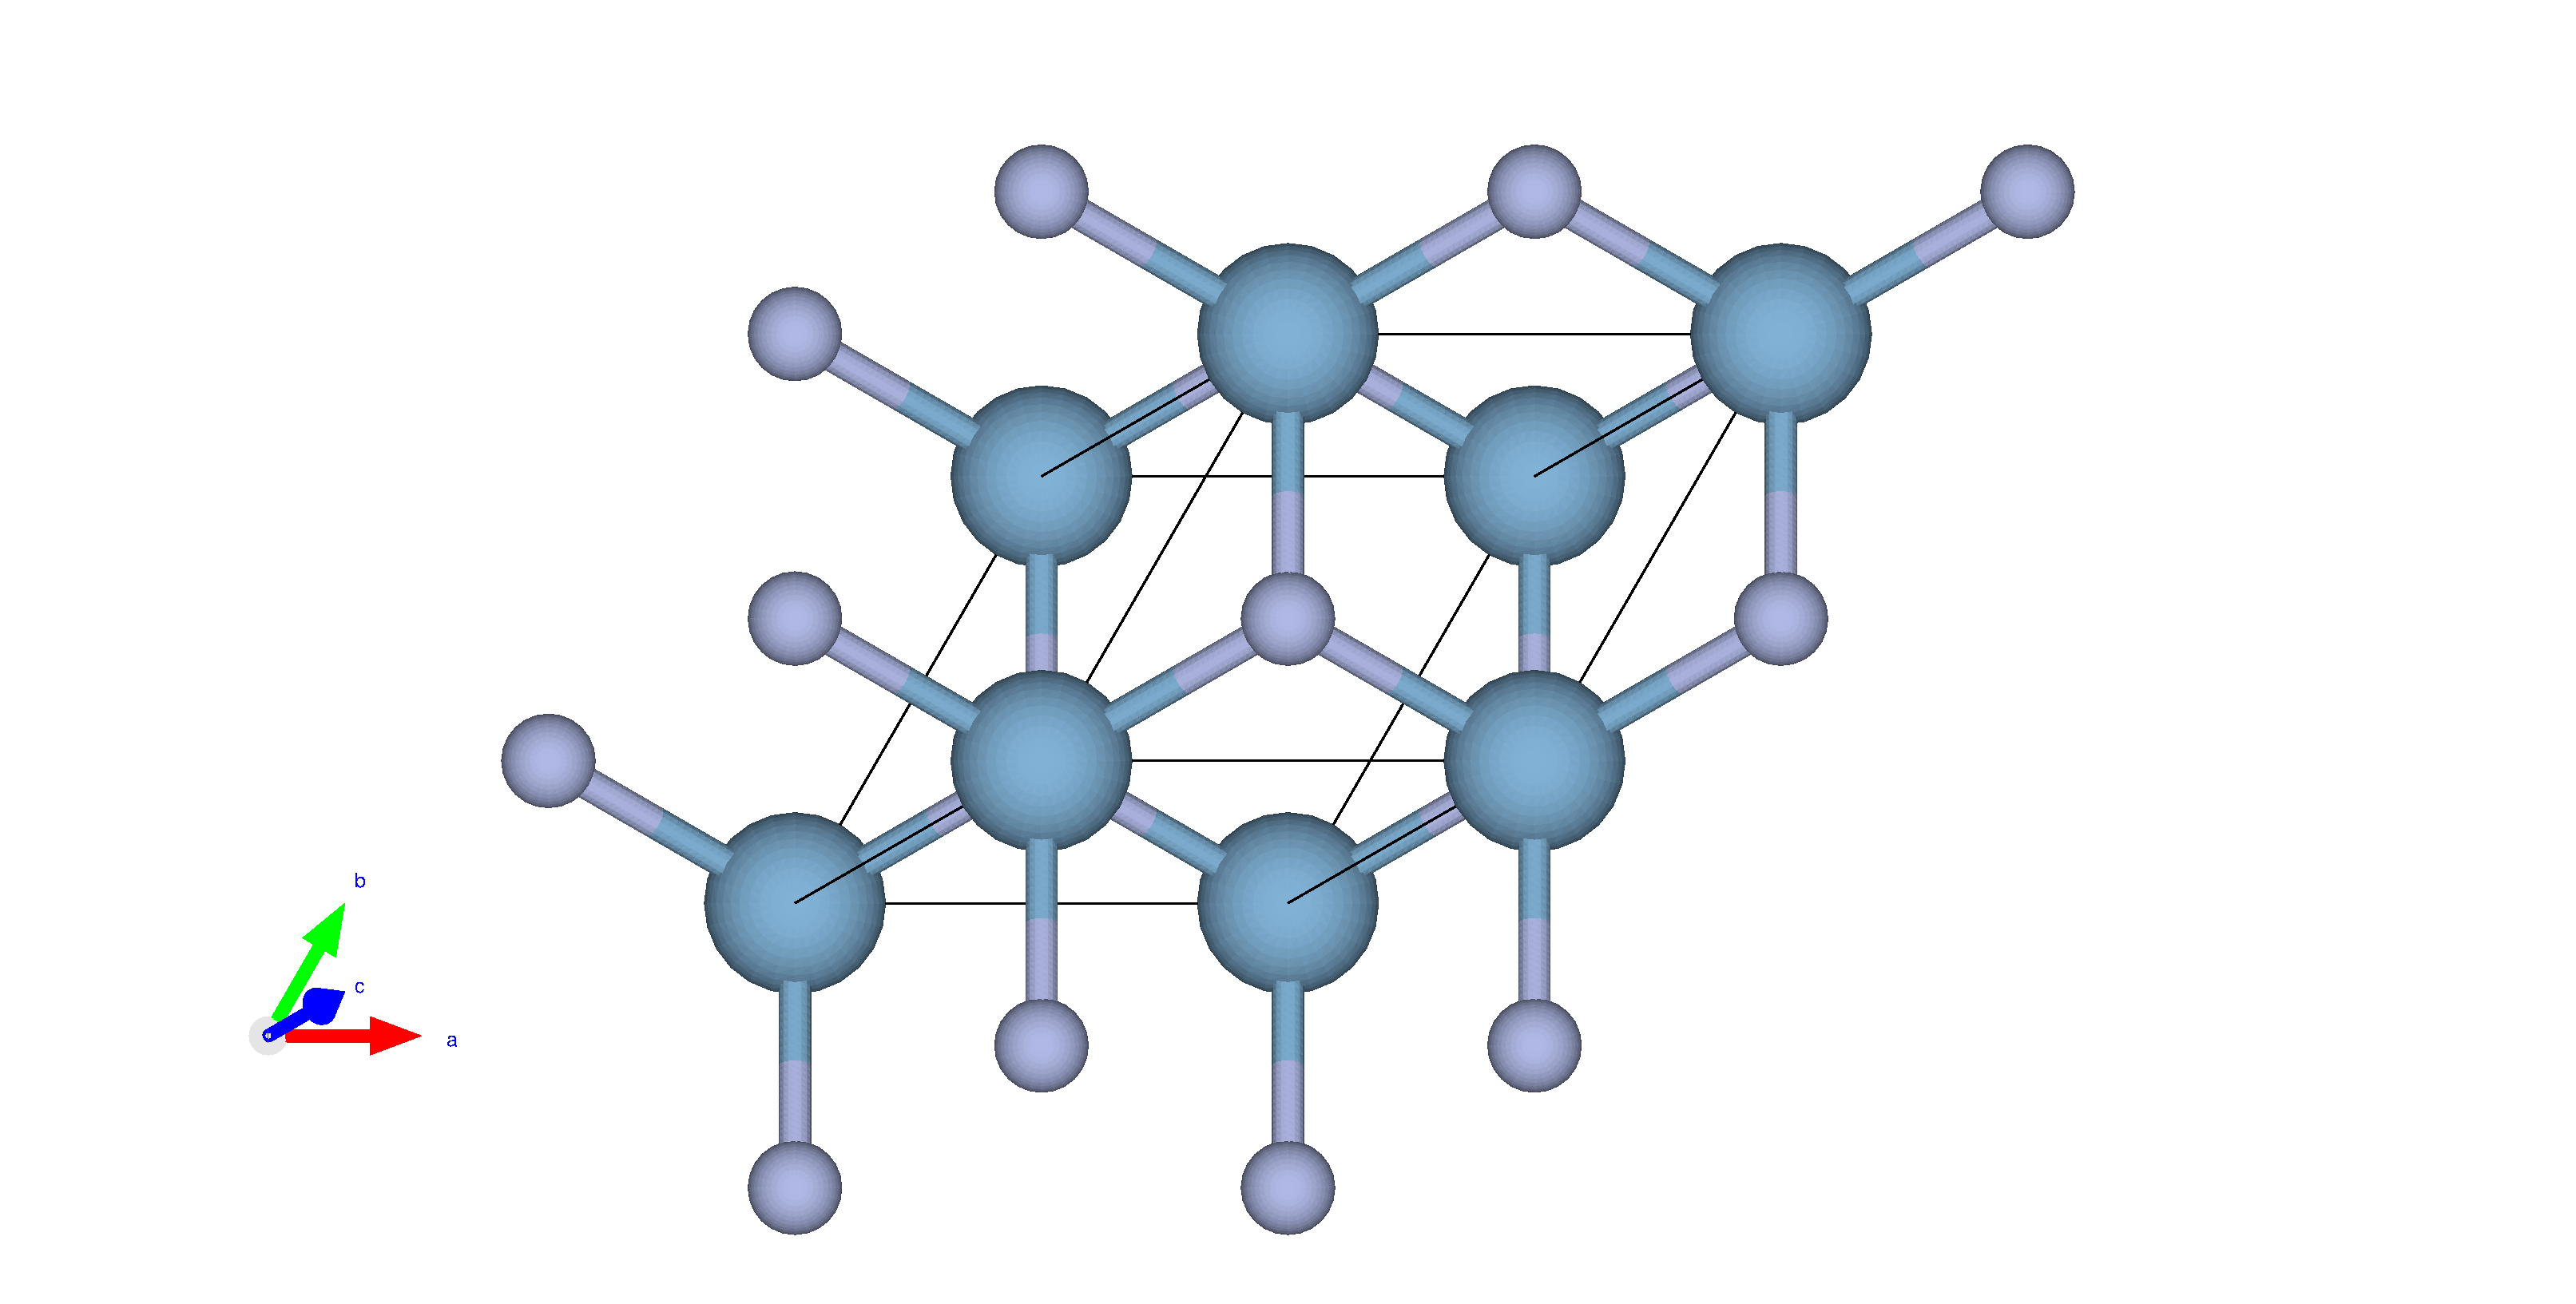
\includegraphics[width=\linewidth]{images/aln_dt_3d.eps}
  \caption{AlN}
\end{subfigure}\hfil % <-- added

\medskip


\caption{Structures of all 3D materials used in this study.}
\label{fig:3d_materials_structure}
\end{figure}


\FloatBarrier
\section{Structural properties}
As mentioned in the previous sections, the DFT method calculates the structures of specific compounds with an accuracy of one percent compared to the experimental results. In particular, the lattice constant was calculated for all materials through the minimization of the total energy, with variations in the lattice parameter plus one relaxation step to precisely determine the positions of the atoms. As one can see, the optimization results are presented in figures \ref{fig:3d_opt} and \ref{fig:2d_opt}, where we can clearly see the parabola that has its minimum point at the equilibrium lattice constant. After the relaxation, the results obtained are shown in tables \ref{tab:lt_ct_2d} and \ref{tab:lt_ct_3d}.

Furthermore, it is important to notice that the lattice constant was not calculated for materials classified as metals by the DFT, for example, $Ge$. In these cases, experimental values are used to obtain a band gap value greater than zero, to proceed with the calculations.

Finally, it is worth noting that these results align well with the values reported in the articles \cite{Matusalem_2020} and \cite{PhysRevB.97.045426}, with the largest deviation being 2.25\% for germanium. This demonstrates a good agreement with the experimental results.

\begin{table}[h]
    \small
    \setlength{\tabcolsep}{5pt} % Adjust cell padding
    \renewcommand{\arraystretch}{1.2} % Adjust row height
    \centering
    \caption{Lattice constants obtained for the three-dimensional materials in this study compared to experimental ones. The experimental constants were obtained from the sources \cite{Matusalem_2020} \cite{article} \cite{alma991022421219705251}.}
    \label{tab:lt_ct_3d}
    \begin{tabular}{c c c}
        \hline
        \hline
        \textbf{Element} & \textbf{Lattice Constant ($\text{\AA}$)} &\textbf{Experimental Lattice Constant ($\text{\AA}$)}  \\
        \hline
        GaN & 4.590 & 4.49\\
        GaP & 5.529 & 5.45\\
        GaAs & 5.760 & 5.65\\
        Ge & 5.78  &5.65\\
        InP & 5.99 & 5.86\\
        Si & 5.468  &  5.43\\
        AlN & 4.401 & 4.37 \\
        \hline
        \hline
    \end{tabular}
\end{table}

\begin{table}[h]
    \small
    \setlength{\tabcolsep}{5pt} % Adjust cell padding
    \renewcommand{\arraystretch}{1.2} % Adjust row height
    \centering
    \caption{Lattice constants obtained for the two-dimensional materials in this study compared to reference ones. The reference values were obtained from the sources \cite{PhysRevB.97.045426}.}
    \label{tab:lt_ct_2d}
    \begin{tabular}{c c c}
        \hline
        \hline
        \textbf{Element} & \textbf{Lattice Constant ($\text{\AA}$)} & \textbf{Reference Lattice Constant ($\text{\AA}$)}  \\
        \hline
        GaN & 3.21 & 3.20\\
        GaP & 3.93 & 3.95 \\
        SiC & 3.10 & 3.09 \\
        GeC & 3.23 & 3.23 \\
        BP & 3.21 &  3.21\\
        BN & 2.51 &  2.51\\
        AlN & 3.12 &  3.12 \\
        \hline
        \hline
    \end{tabular}
\end{table}

\begin{figure}[htb]
    \centering % <-- added
\begin{subfigure}{0.45\textwidth}
  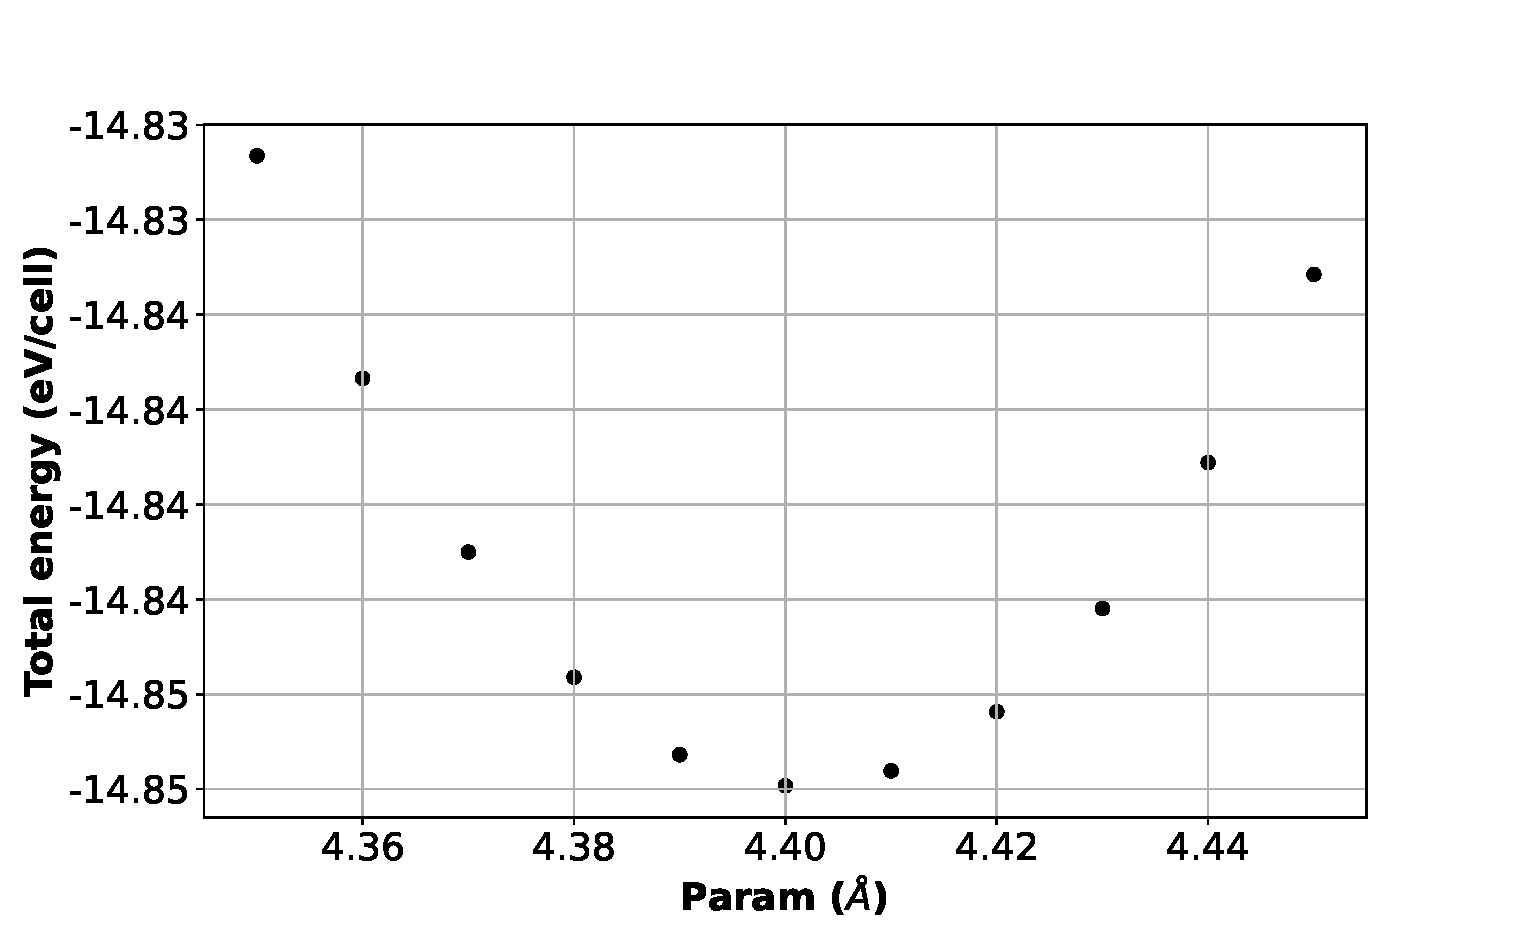
\includegraphics[width=\linewidth]{images/aln_3d_opt.eps}
  \caption{AlN}
\end{subfigure}\hfil % <-- added
\begin{subfigure}{0.45\textwidth}
  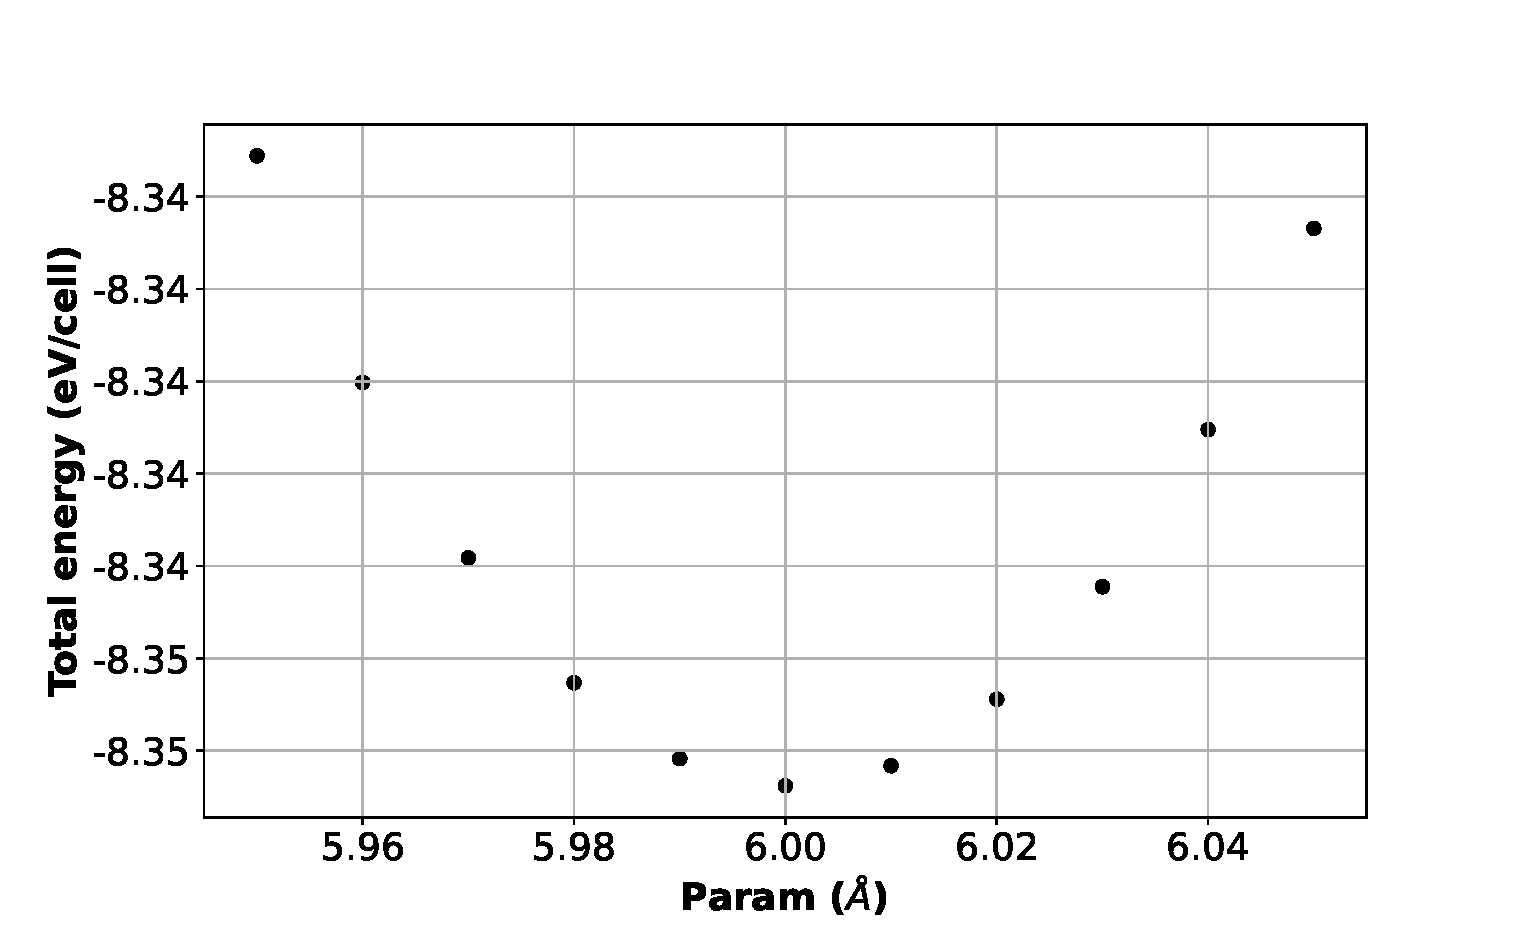
\includegraphics[width=\linewidth]{images/inp_3d_opt.eps}
  \caption{InP}
\end{subfigure}

\medskip

\begin{subfigure}{0.45\textwidth}
  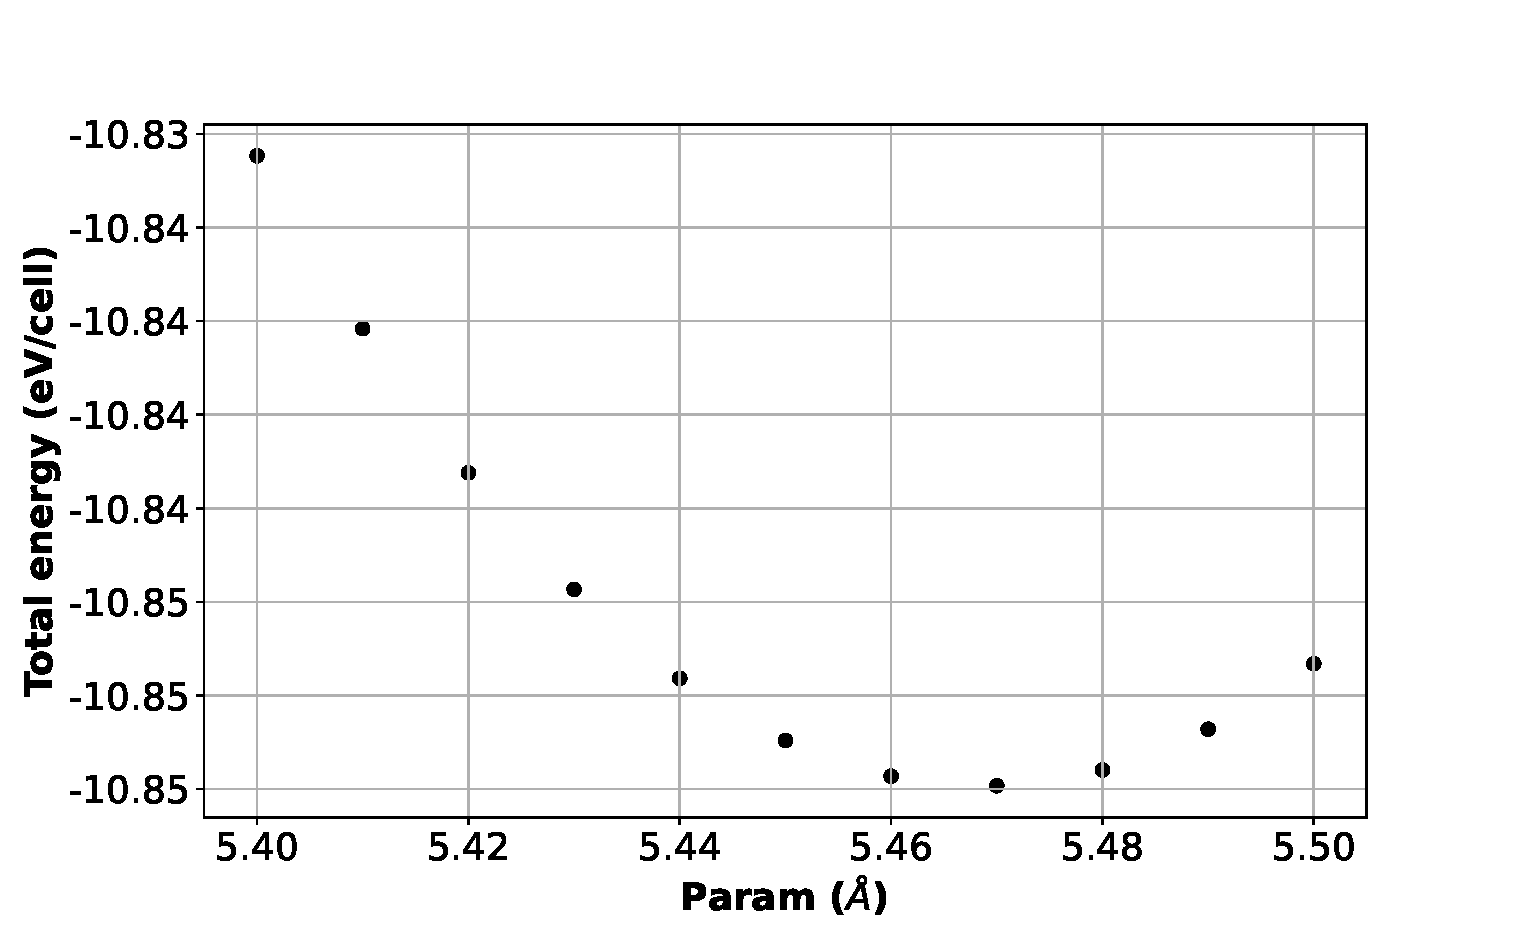
\includegraphics[width=\linewidth]{images/si_3d_opt.eps}
  \caption{Si}
\end{subfigure}\hfil % <-- added
\begin{subfigure}{0.45\textwidth}
  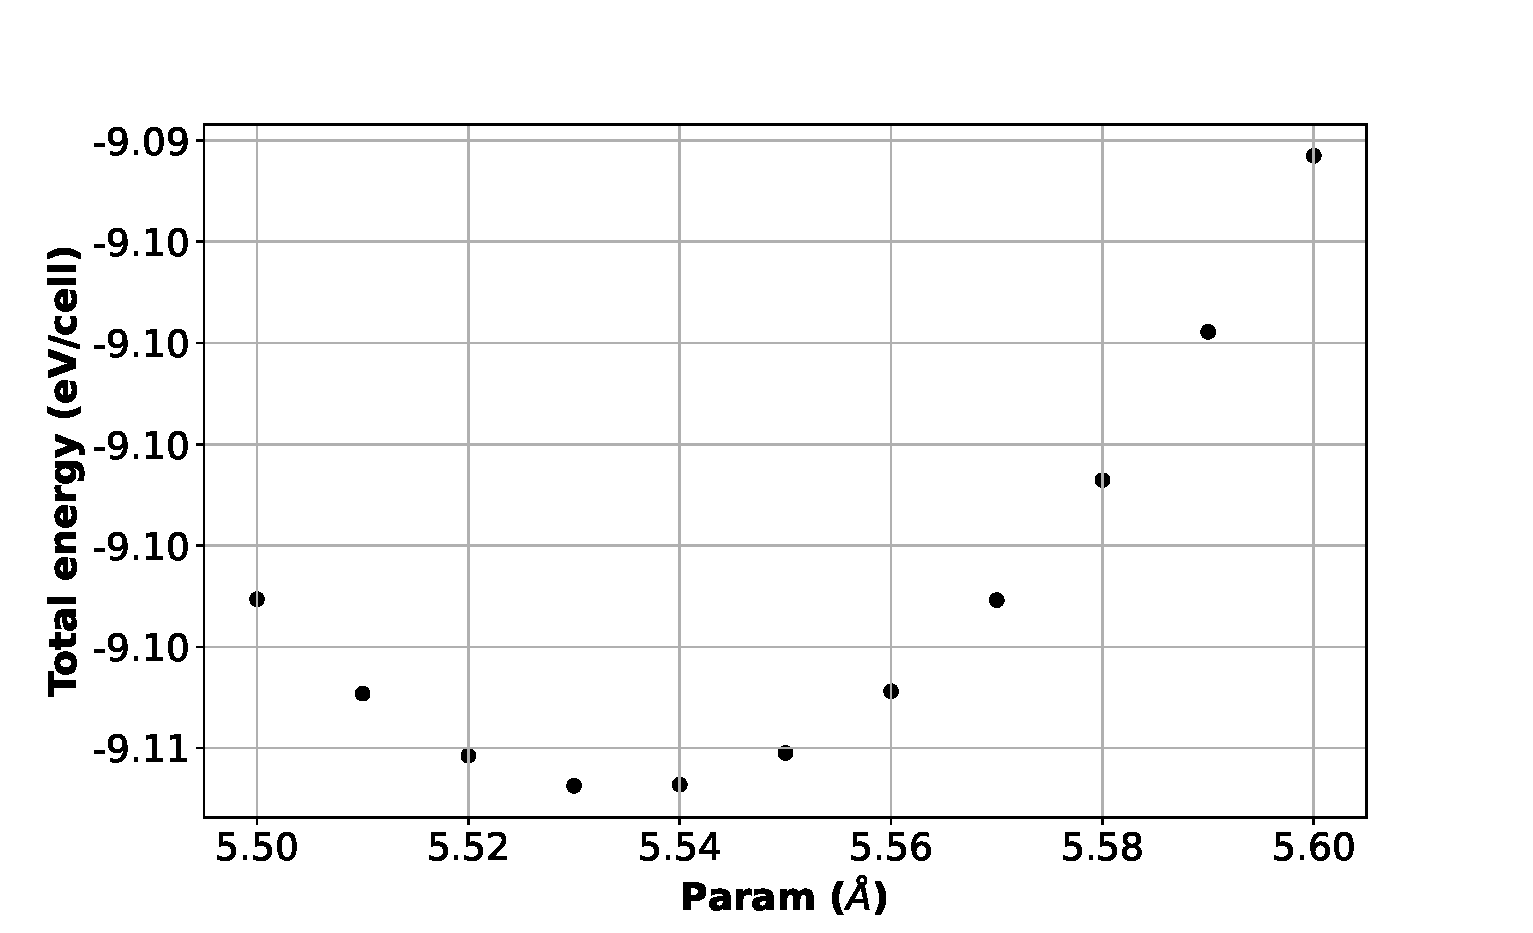
\includegraphics[width=\linewidth]{images/gap_3d_opt.eps}
  \caption{GaP}
\end{subfigure}\hfil % <-- added

\medskip

\begin{subfigure}{0.45\textwidth}
  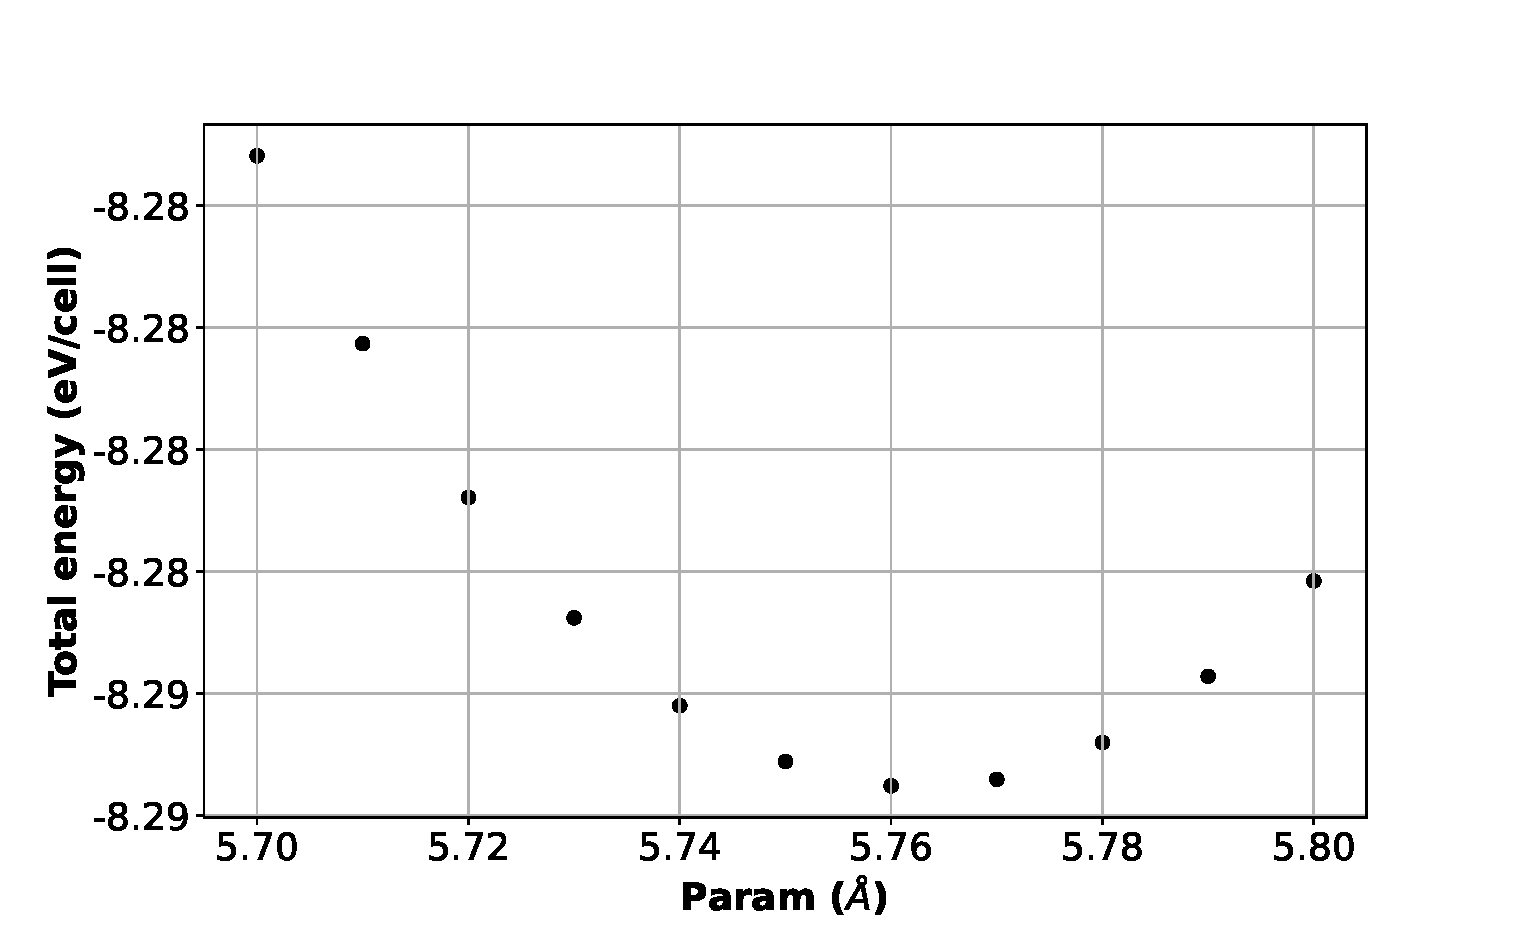
\includegraphics[width=\linewidth]{images/gaas_3d_opt.eps}
  \caption{GaAs}
\end{subfigure}\hfil % <-- added
\begin{subfigure}{0.45\textwidth}
  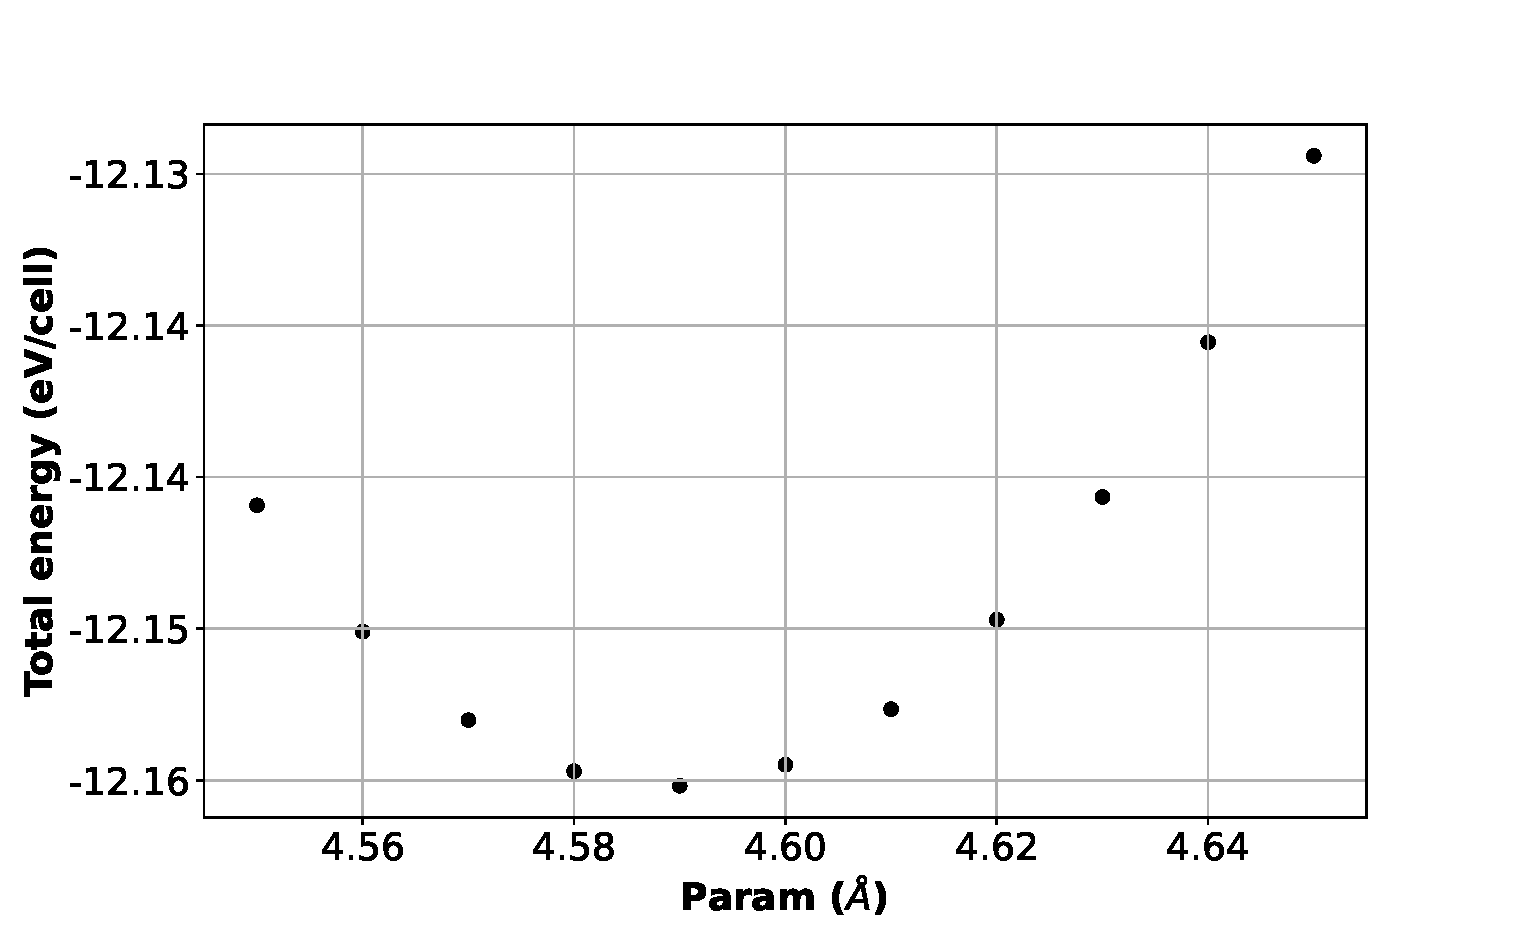
\includegraphics[width=\linewidth]{images/gan_3d_opt.eps}
  \caption{GaN}
\end{subfigure}

\medskip


\caption{Lattice constant versus total energy for all 3D materials used in this study.}
\label{fig:3d_opt}
\end{figure}

\begin{figure}[htb]
    \centering % <-- added
\begin{subfigure}{0.45\textwidth}
  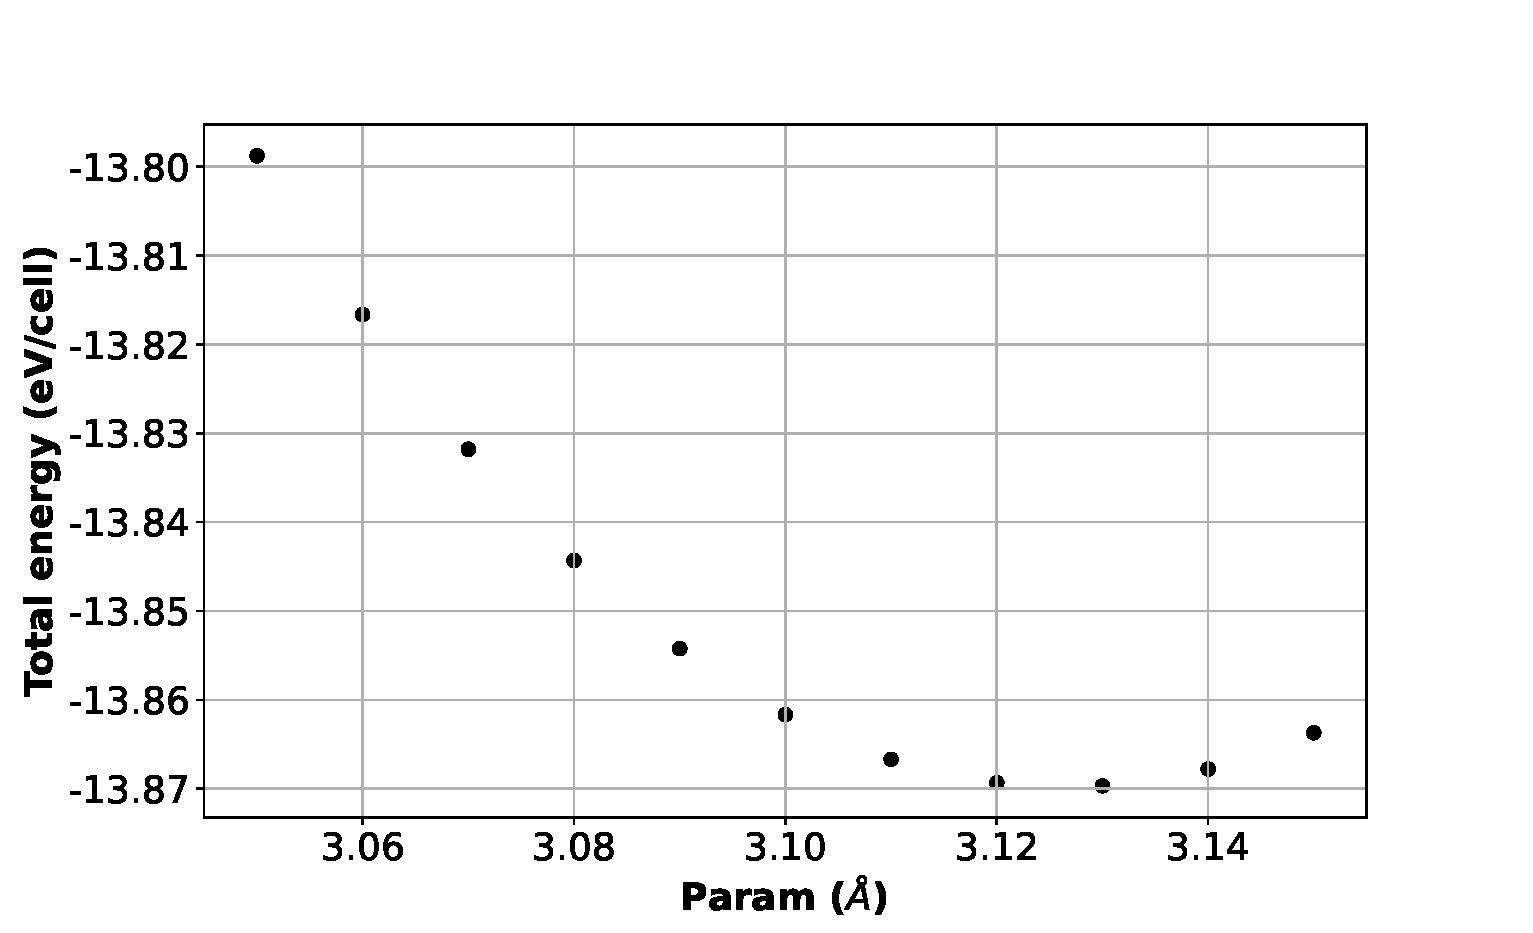
\includegraphics[width=\linewidth]{images/aln_2d_opt.eps}
  \caption{AlN}
\end{subfigure}\hfil % <-- added
\begin{subfigure}{0.45\textwidth}
  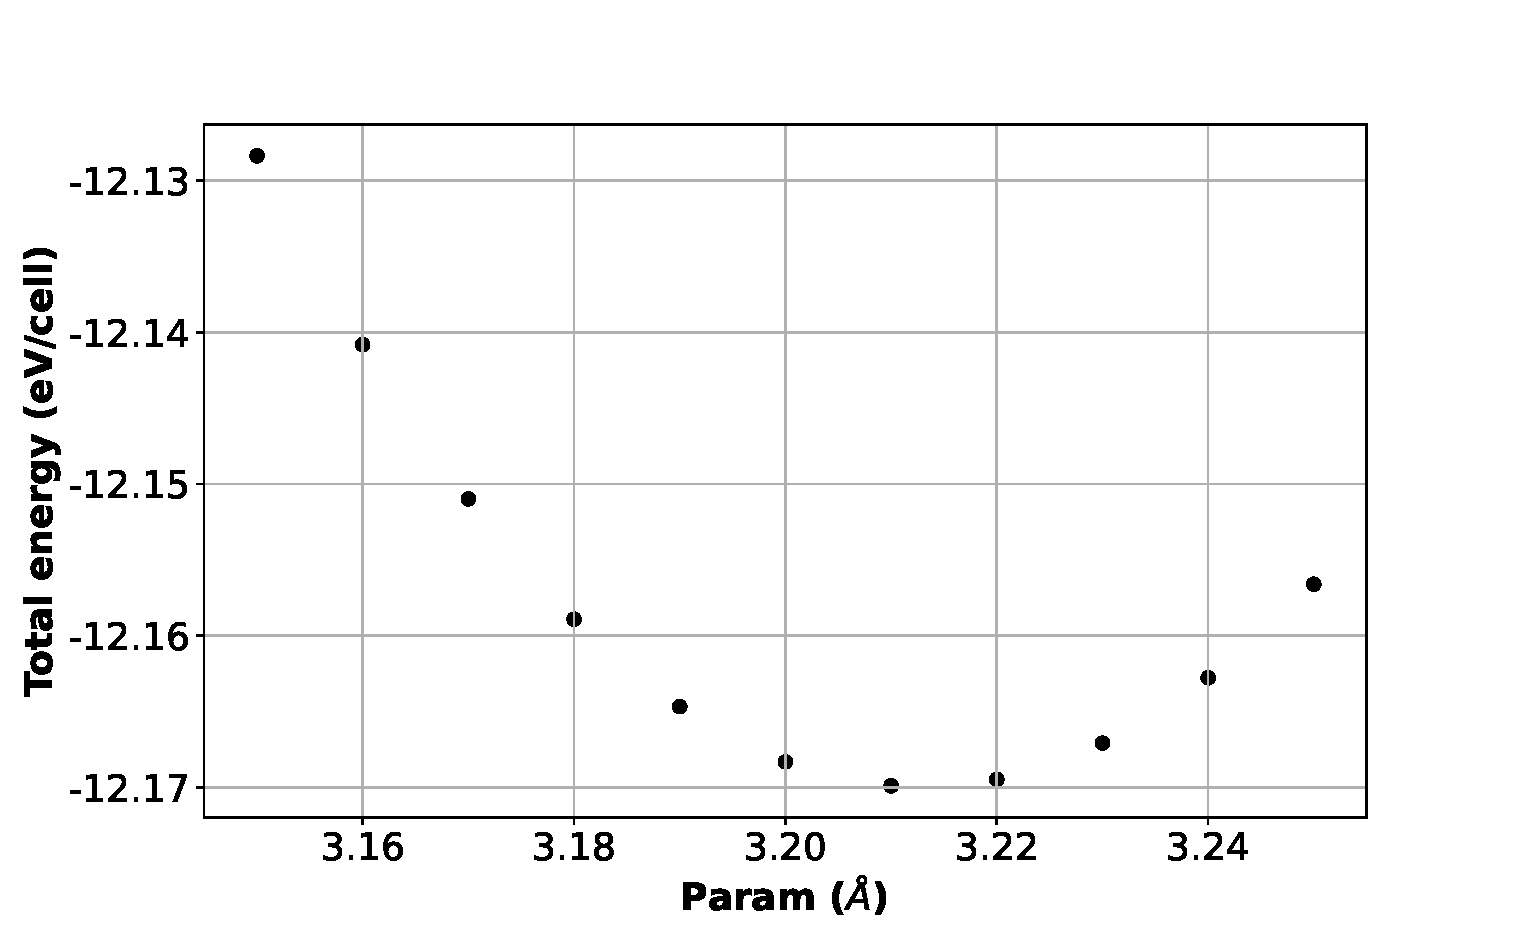
\includegraphics[width=\linewidth]{images/bp_2d_opt.eps}
  \caption{BP}
\end{subfigure}

\medskip

\begin{subfigure}{0.45\textwidth}
  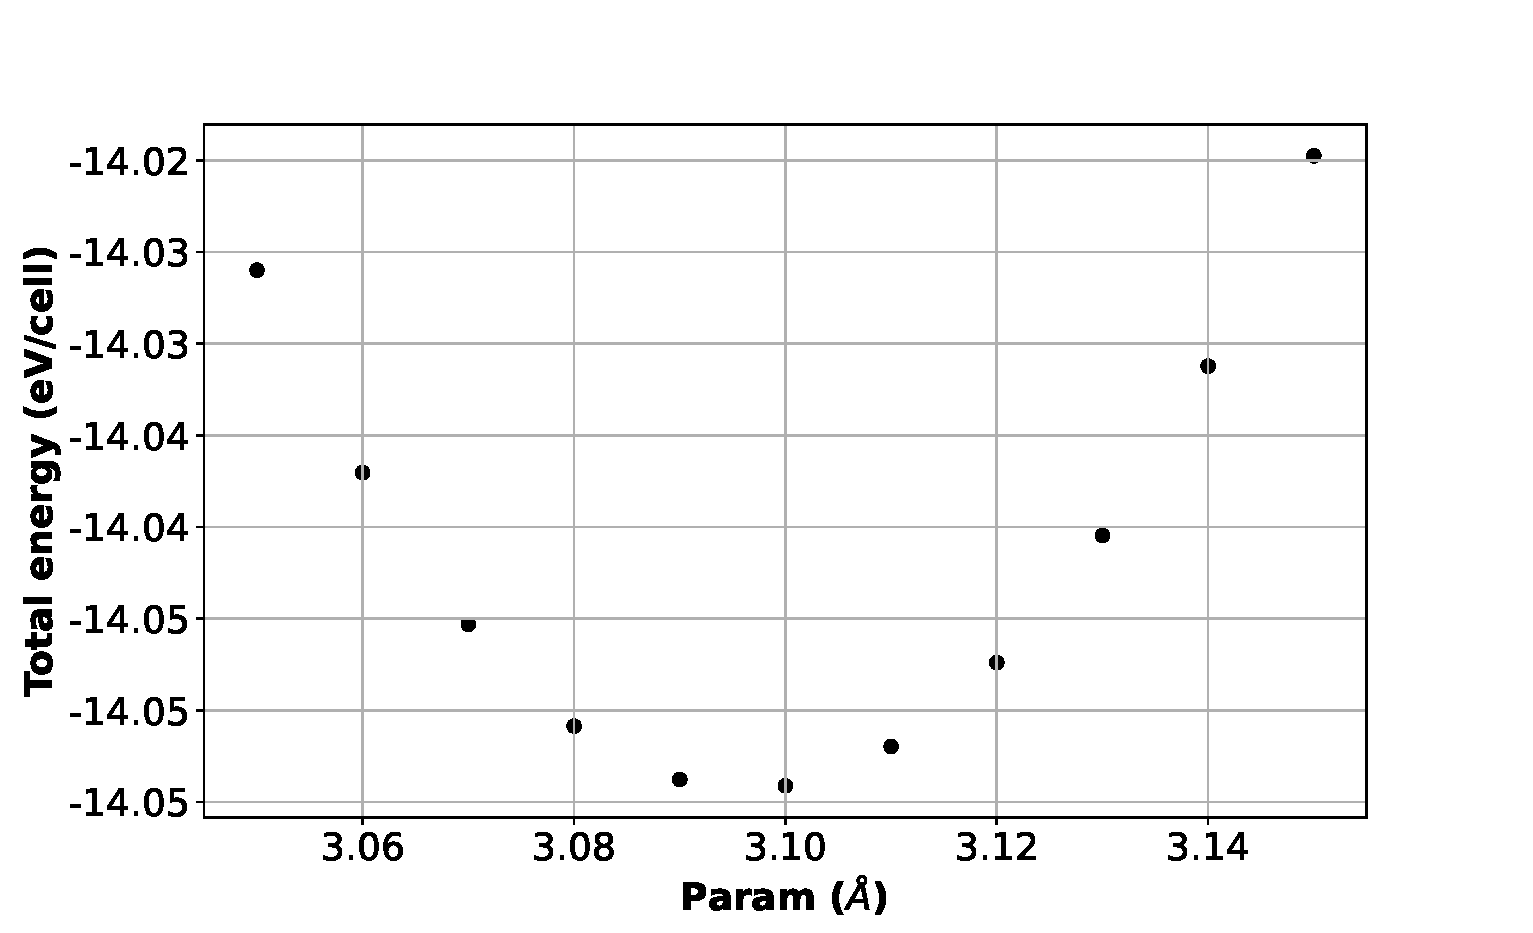
\includegraphics[width=\linewidth]{images/sic_2d_opt.eps}
  \caption{SiC}
\end{subfigure}\hfil % <-- added
\begin{subfigure}{0.45\textwidth}
  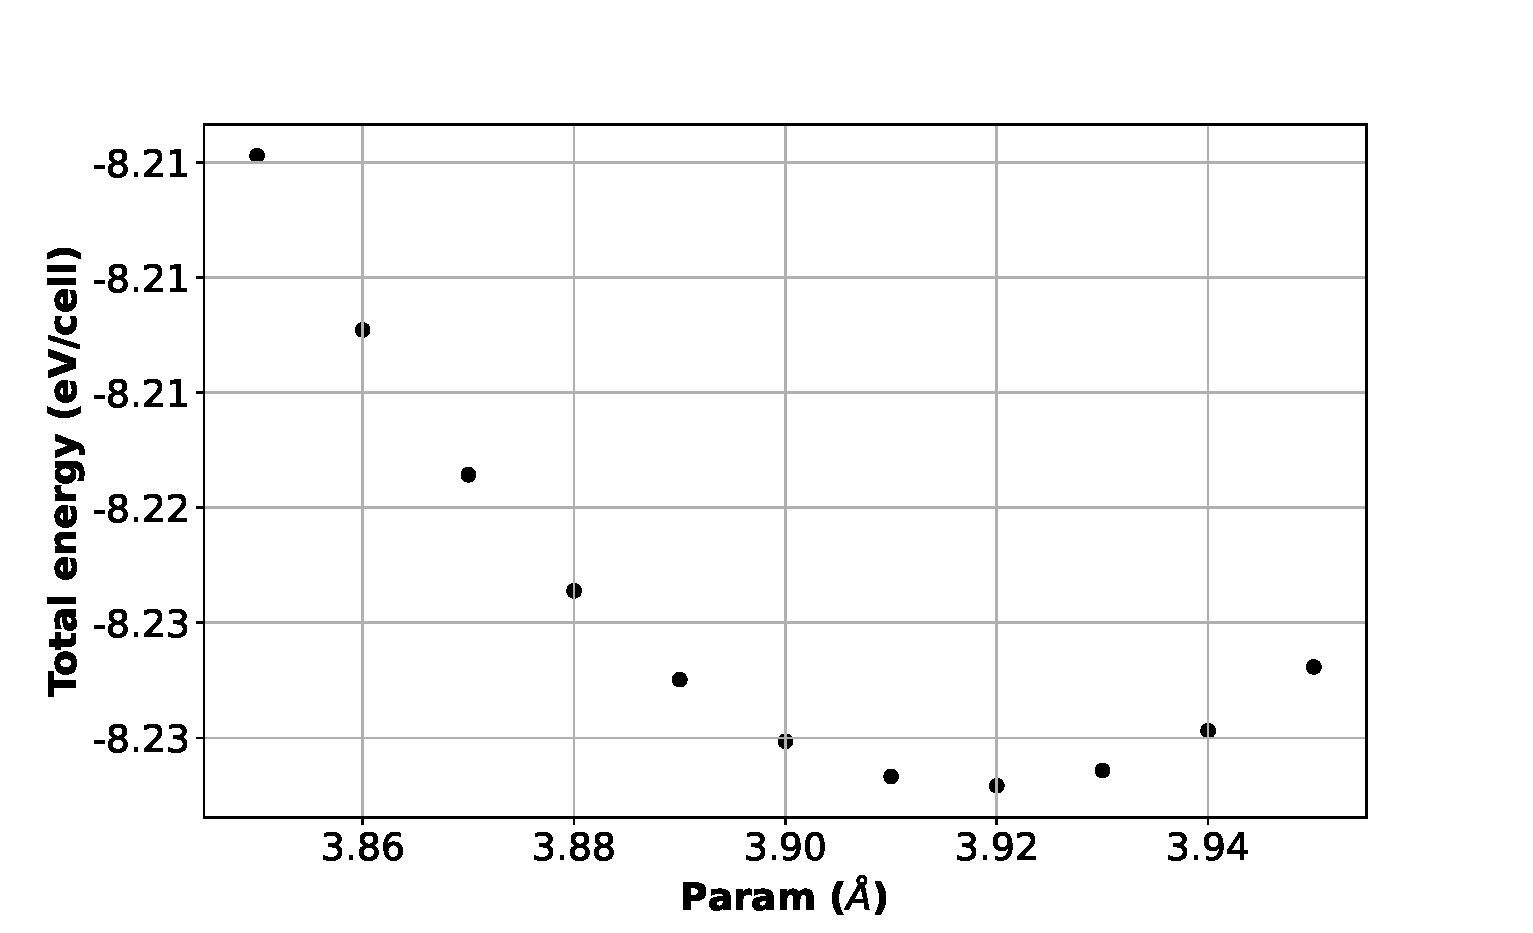
\includegraphics[width=\linewidth]{images/gap_2d_opt.eps}
  \caption{GaP}
\end{subfigure}\hfil % <-- added

\medskip

\begin{subfigure}{0.45\textwidth}
  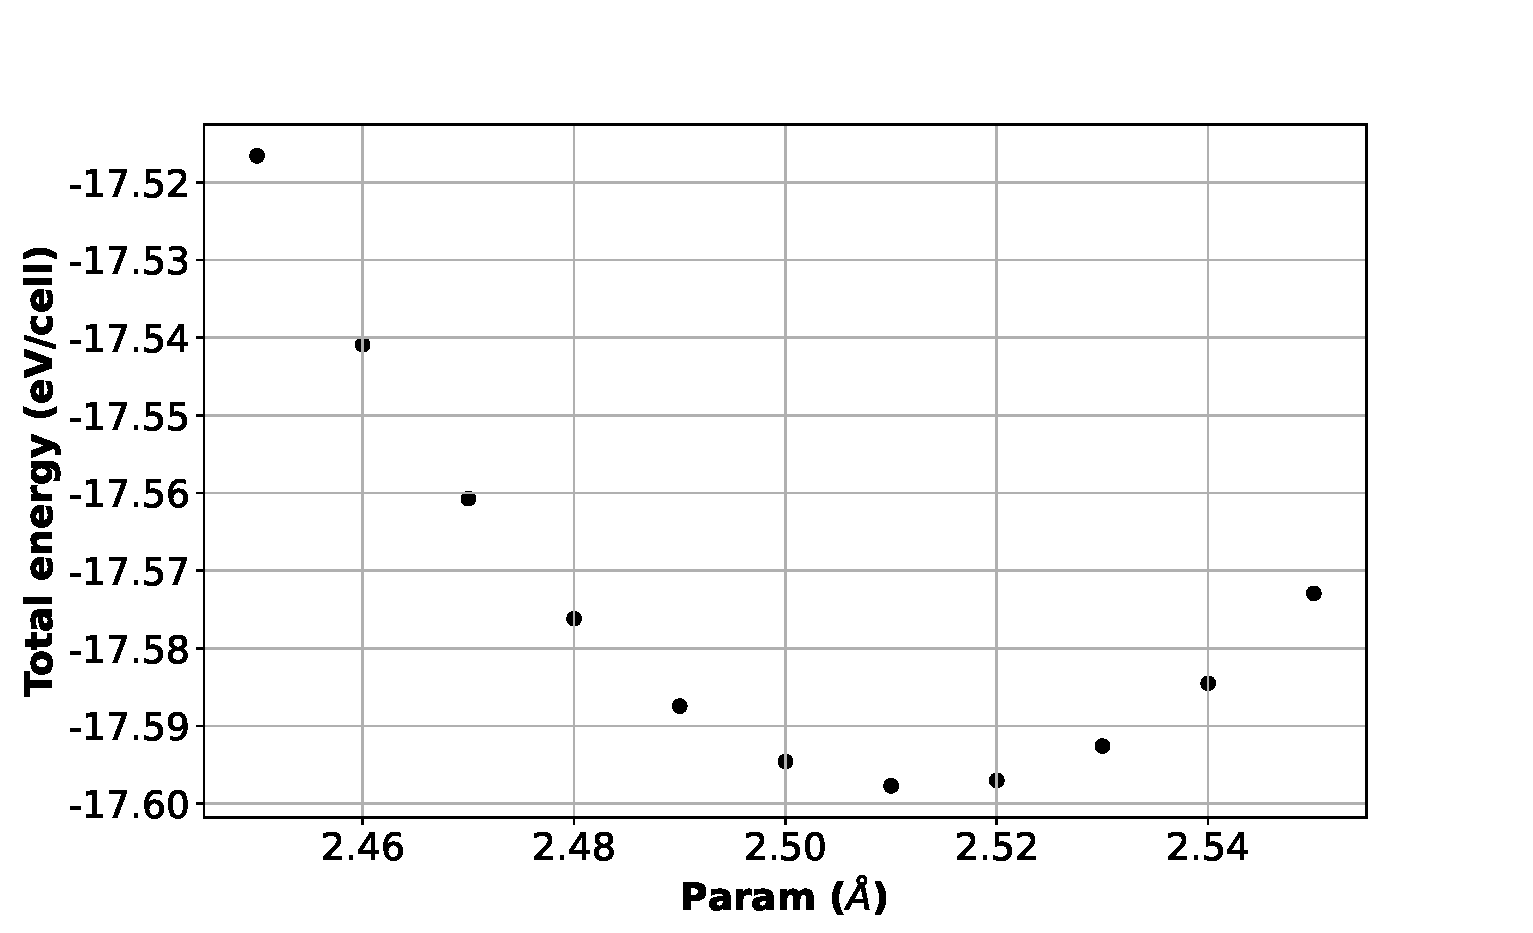
\includegraphics[width=\linewidth]{images/bn_2d_opt.eps}
  \caption{BN}
\end{subfigure}\hfil % <-- added
\begin{subfigure}{0.45\textwidth}
  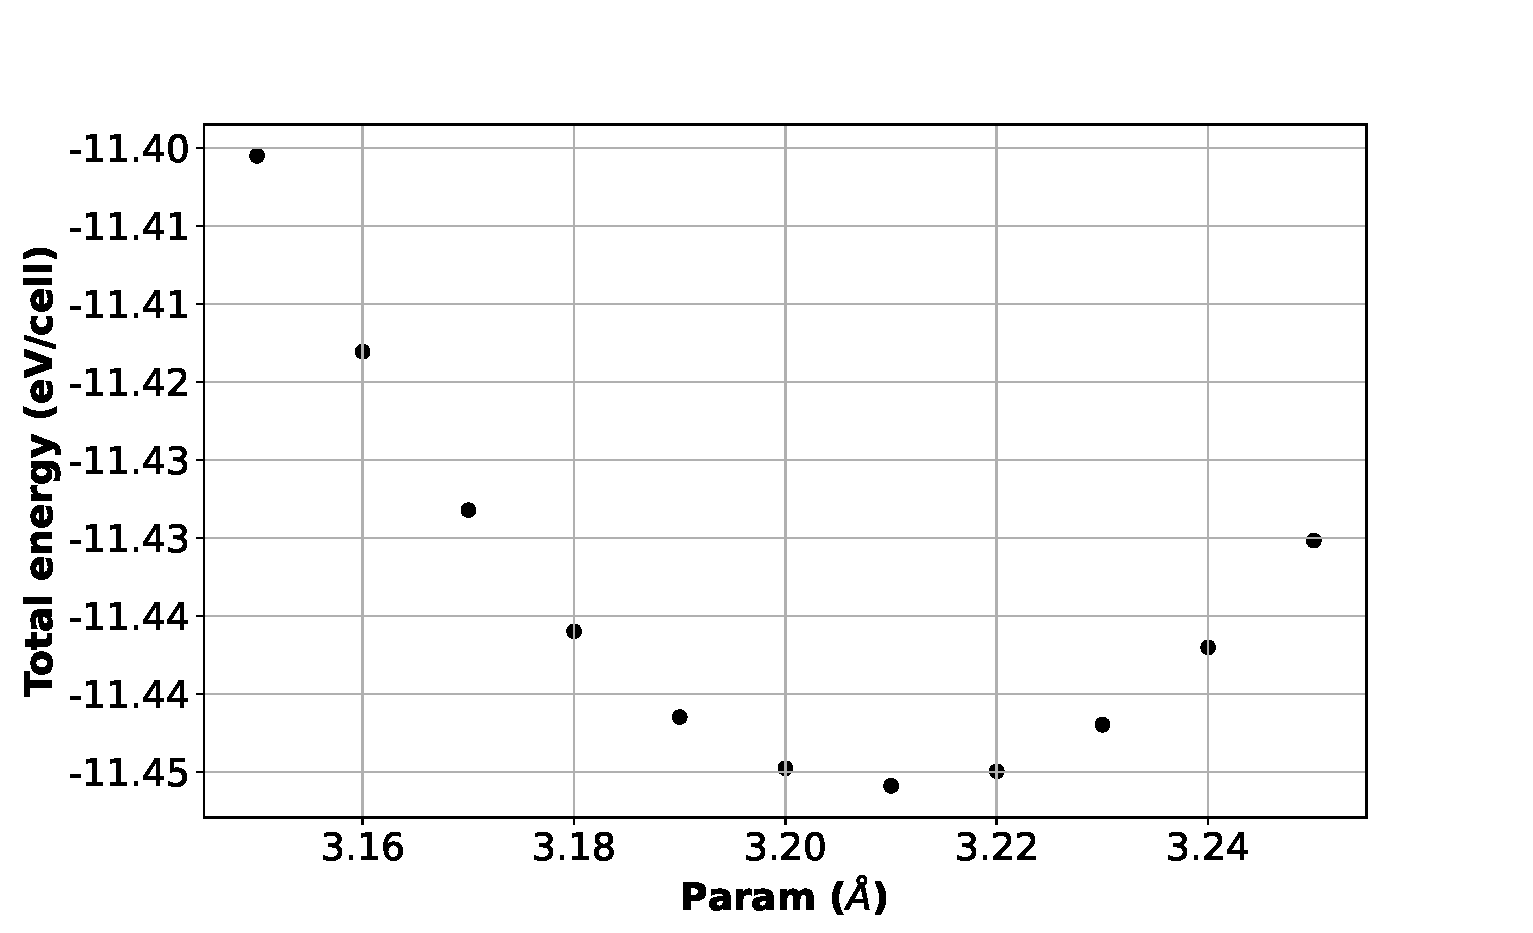
\includegraphics[width=\linewidth]{images/gan_2d_opt.eps}
  \caption{GaN}
\end{subfigure}

\medskip
\begin{subfigure}{0.45\textwidth}
  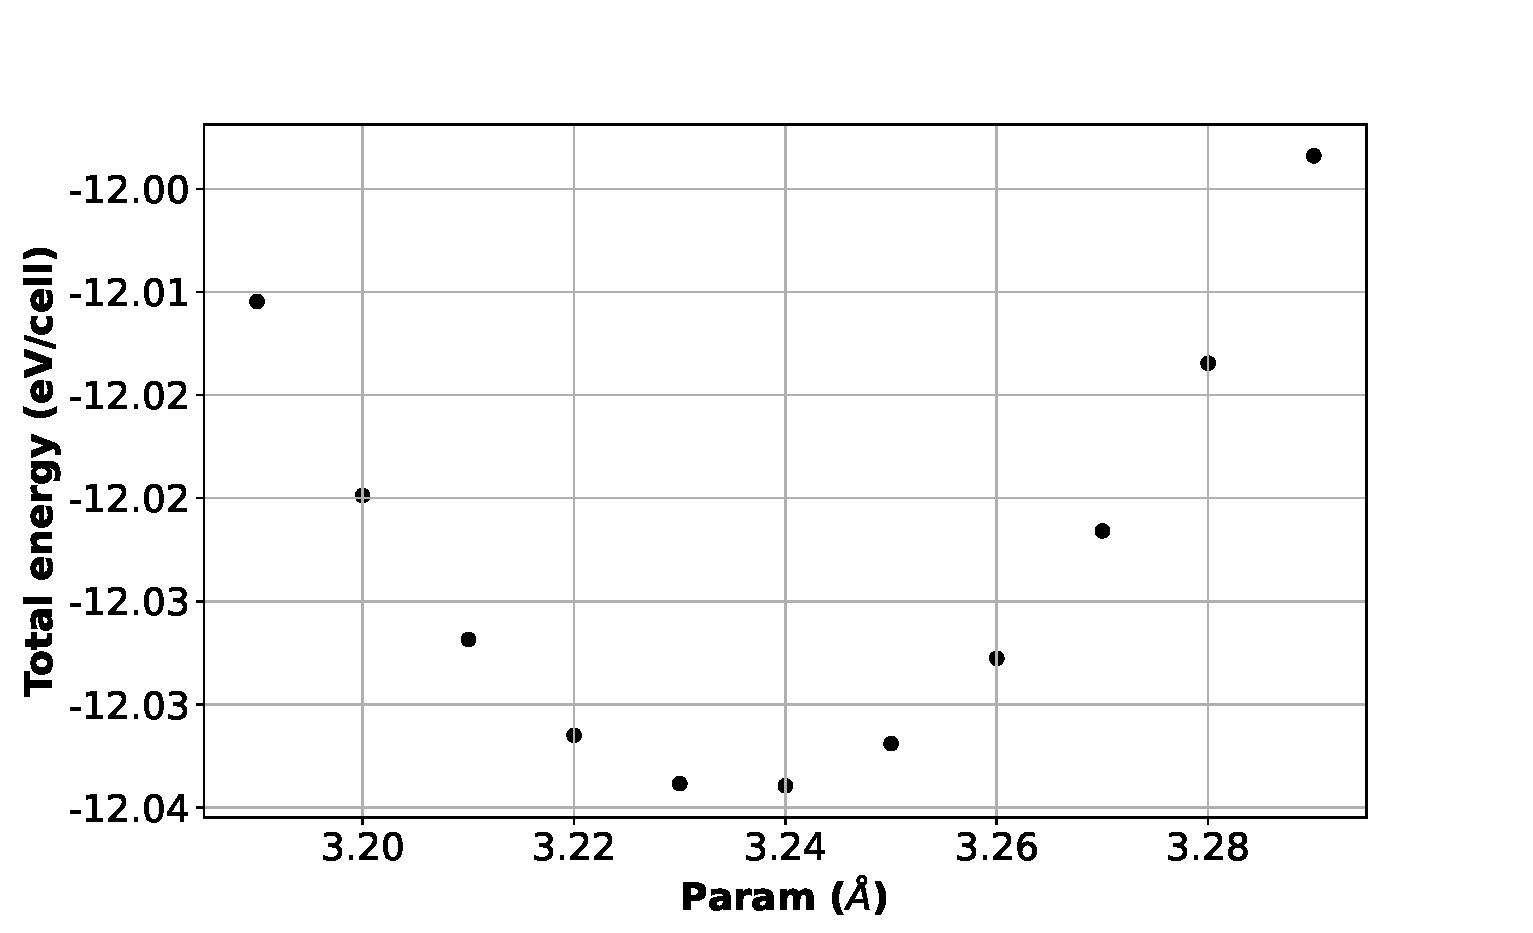
\includegraphics[width=\linewidth]{images/gec_2d_opt.eps}
  \caption{GeC}
\end{subfigure}

\medskip


\caption{Lattice constant versus total energy for all 2D materials used in this study.}
\label{fig:2d_opt}
\end{figure}



\FloatBarrier
\section{Electronic properties}

With the intention of creating a benchmark, an attempt was made to replicate some of the articles that employed the DFT -1/2 method. The first article is from 2020 \cite{Matusalem_2020}, in which several 3D materials were simulated, and the second is from 2018 \cite{PhysRevB.97.045426}, in which various 2D materials were simulated.

For these materials, one uses the Minushalf software to calculate the band character. When one looks at the results, we notice that some elements, like three-dimensional Si, has the band character focused on one orbital. Others, like three-dimensional $GaN$ , has the character spread out among the orbitals. This is important because it determines which correction to use. For example, if a band has its character centered on one orbital, we apply a correction that extracts the electron potential only from that orbital. On the other hand, if the character is spread across multiple orbitals, one distributes the correction among them, possibly even on different atoms. One can see these results in Figures \ref{fig:3d_compounds_character} and \ref{fig:2d_compounds_character}. It's worth mentioning that characters contributing less than 10 percent aren't labeled, but they're still shown in the charts.

Next, one employed the `execute'' command to perform the calculation, yielding the band gaps resulting from the DFT-1/2 method and the respective cutoff values as presented in the table. As part of the calculation, one also determined whether the calculation would consider a direct or indirect band gap. The results are listed in Tables \ref{tab:3d_compounds_results} and \ref{tab:2d_compounds_results}. It is worth noting that in the cutoff result, one lists the compound symbol, the orbital to which the cutoff was applied, and the amplitude used in the calculation. Positive amplitudes indicate valence correction, while negative amplitudes indicate conduction correction. Some interesting patterns that one can find include the observation that the valence correction is always less than the results obtained with the addition of the conduction correction. This is due to the fact that the conduction correction makes the energy level of the first conduction band go up, which increases the band gap. On the other hand, the extent to which the band gap increases depends on the localization of the band. Compounds with a more localized character in a given orbital have much larger corrections than compounds in which the character is distributed. For example, one can mention the material $BP$ $2D$, which experienced a $60\%$ increase in the gap when the conduction band correction was applied, whereas the $GaP$ $2D$ compound had a $14\%$ increase. The main difference is that the $BP$ $2D$ band is concentrated in the boron $p$ orbital, while the $GaP$ band is divided between the $s$ orbitals of the two atoms.

To assess the agreement between the experimental data and the obtained results, we calculated the root mean squared error (RMSE) relative to the experimental values for 3D materials. In the case of 2D materials, GW values were employed for comparison, as not all of these compounds have available experimental data. Upon examining the RMSE results, it becomes apparent that the outcomes produced by Minushalf exhibit much closer agreement compared to those from the DFT method. In 2D materials, we observe that the DFT-1/2 with valence correction yields a score more than three times lower than the DFT score, while the valence correction is more than two times higher. This indicates that the valence results closely align with the GW values, whereas the conduction correction occasionally overestimates the band gap. On the other hand, the corrections applied to the 3D materials demonstrate a score two times lower with the DFT-1/2, indicating a closer match to the reference values. One crucial detail to note is the clear deviation of the DFT results below the identity line, confirming the hypothesis that the DFT underestimates the band gap, as stated in the methodology section. These findings strongly suggest the superiority of the former method. The corresponding charts can be seen in Figures \ref{fig:2d_comparison} and \ref{fig:3d_comparison}.

Subsequently, band structures were generated, providing crucial insights into the compounds under investigation. These plots visually demonstrate how the correction impacts the band gaps and modifies the bands of the studied compounds. Additionally, it is imperative to scrutinize the positions of the VBM and CBM, indicated by the red dots, to affirm the coherence of the results. For instance, in the case of $GaN$ 3D, it is evident that the compound possesses a direct band gap at the gamma point. It is also noteworthy how the bands are distinctly separated and how the band gap expands with the application of a correction. It is important to mention that when the Fermi energy is set at zero, we exclusively observe movement in the conduction band in the charts depicted in Figures \ref{fig:2d_compounds_bands} and \ref{fig:3d_compounds_bands}

Finally, the sensitivity of the electronic properties of the materials in relation to their structure may have led to some minor discrepancies in comparison to the results and the referenced articles. These discrepancies can arise from both the varying relaxation conditions of the material and the different techniques used to approximate the exchange-correlation functionals utilized in the calculations.

\begin{table}[h]
    \small
    \setlength{\tabcolsep}{5pt} % Adjust cell padding
    \renewcommand{\arraystretch}{1.2} % Adjust row height
    \centering
    \caption{Table comparing the obtained DFT -1/2 Gap values of three-dimensional compounds with the experimental results and the standard DFT method. The table also displays the cutoffs obtained at each step of the process, along with tags indicating the type of correction and whether the considered gap is direct or indirect. Experimental values were obtained from \cite{Matusalem_2020}.}
    \label{tab:3d_compounds_results}
    \begin{tabular}{c c c l p{3.5cm} c}
        \hline
        \hline
        \textbf{Element} & \textbf{GGA (eV)} & \textbf{Expt. (eV)} & \textbf{Tags} & \textbf{CUT (a.u.)} & \textbf{DFT-1/2 (eV)} \\
        \hline
        AlN  & 3.00 & 6.23 &direct,$v$  & (N,l=p,A=1):2.88 & 5.85 \\
        
        GaAs & 0.10 & 1.42 & direct,$v$ & (As,l=p,A=1):3.79 & 1.09  \\
        
        
        GaN & 1.37 & 3.50 & direct,$v$  & (N,l=p,A=1):3.02 & 3.13 \\
    
        
        GaP & 1.46 & 2.78 & direct,$v+cf$  & (P,l=p,A=1):3.63 (Ga,l=s,A=-1):2.73 (P,l=s,A=-1):1.76 & 2.91 \\
    
        & & 0.80 & direct,$v+c$ & (Ge,l=p,A=1):4.04 (Ge,l=s,A=-1):2.29 & 0.92 \\
        \multirow{-2}{*}{Ge}& \multirow{-2}{*}{metal} & 0.66 &indirect,$v+c$ & (Ge,l=p,A=1):4.06 (Ge,l=s,A=-1):1.93 & 0.87 \\

    
        & & &direct,$v$  & (P,l=p,A=1):3.91  & 1.52 \\
        \multirow{-2}{*}{InP} & \multirow{-2}{*}{0.326} & \multirow{-2}{*}{1.34} & direct,$vf$  & (In,l=d,A=1):8.42 (In,l=p,A=1):0.03  (P,l=p,A=1):3.92 & 1.24 \\
        
        & 2.55 & 3.40 & direct,$v$ & (Si,l=p,A=1):3.69 & 2.94\\
        \multirow{-2}{*}{Si}& 0.62 & 1.20 & indirect,$v$ & (Si,l=p,A=1):3.60  & 1.42 \\
        \hline
        \hline
    \end{tabular}
    
\end{table}

\begin{table}[h]
    \small
    \setlength{\tabcolsep}{5pt} % Adjust cell padding
    \renewcommand{\arraystretch}{1.2} % Adjust row height
    \caption{Table comparing the obtained DFT -1/2 Gap values of two-dimensional compounds with the GW results and the standard DFT method. The table also displays the cutoffs obtained at each step of the process, along with tags indicating the type of correction and whether the considered gap is direct or indirect. GW results were obtained from \cite{PhysRevB.97.045426}.}
    \label{tab:2d_compounds_results}
  
    \begin{tabular}{c c c l p{3.5cm} c}
        \hline
        \hline
        \textbf{Element} & \textbf{GGA (eV)} & \textbf{GW (eV)} & \textbf{Tags} & \textbf{CUT (a.u.)} & \textbf{DFT-1/2 (eV)} \\
        \hline
        & & &  indirect, $v$  & (N,l=p,A=1):2.80 & 6.64  \\
        \multirow{-2}{*}{AlN} & \multirow{-2}{*}{2.91}  & \multirow{-2}{*}{5.57} & indirect, $v+c$   & (N,l=p,A=1):2.80 (N,l=s,A=-1):0.00 & 7.18\\
        

        & & & direct, $v$    & (N,l=p,A=1):2.52 & 6.62\\
        \multirow{-2}{*}{BN} & \multirow{-2}{*}{4.65}  & \multirow{-2}{*}{6.86} &direct, $v+c$  & (N,l=p,A=1):2.52 (B,l=p,A=-1):1.85 & 7.54 \\

        
        & & &direct, $v$  & (P,l=p,A=1):3.26 & 1.90  \\
        \multirow{-2}{*}{BP} & \multirow{-2}{*}{0.90} & \multirow{-2}{*}{1.81} & direct, $v+c$   & (P,l=p,A=1):3.26 (B,l=p,A=-1):3.26 & 3.04 \\


        & & & indirect, $v$  & (N,l=p,A=1):3.10 & 3.63 \\
        \multirow{-2}{*}{GaN} & \multirow{-2}{*}{2.156} & \multirow{-2}{*}{4.10} & indirect, $v+c$  & (N,l=p,A=1):3.10 (N,l=s,A=-1):1.15 &3.73  \\
        
        
        & & & indirect, $v$  &  (P,l=p,A=1):3.19 & 2.98   \\
        \multirow{-2}{*}{GaP} & \multirow{-2}{*}{1.20} & \multirow{-2}{*}{3.80} & indirect, $v+c$   &  (P,l=p,A=1):3.19  (P,l=p,A=-1):2.65& 3.41 \\

        
        & & & direct, $v$ & (C,l=p,A=1):3.20 & 3.43   \\
        \multirow{-2}{*}{GeC} & \multirow{-2}{*}{2.09} & \multirow{-2}{*}{3.83} & direct, $v+c$   & (C,l=p,A=1):3.20 (Ge,l=p,A=-1):3.15 & 4.25  \\
        
        & & &  indirect, $v$  & (C,l=p,A=1):3.13& 3.90  \\
        \multirow{-2}{*}{SiC} & \multirow{-2}{*}{2.54} & \multirow{-2}{*}{4.42} &  indirect, $v+c$ & (C,l=p,A=1):3.13 (Si,l=p,A=-1):2.75 & 4.37  \\
        \hline
        \hline
    \end{tabular}
    
\end{table}


\begin{figure}[!ht]
        \centering % <-- added
\begin{subfigure}{0.3\textwidth}
  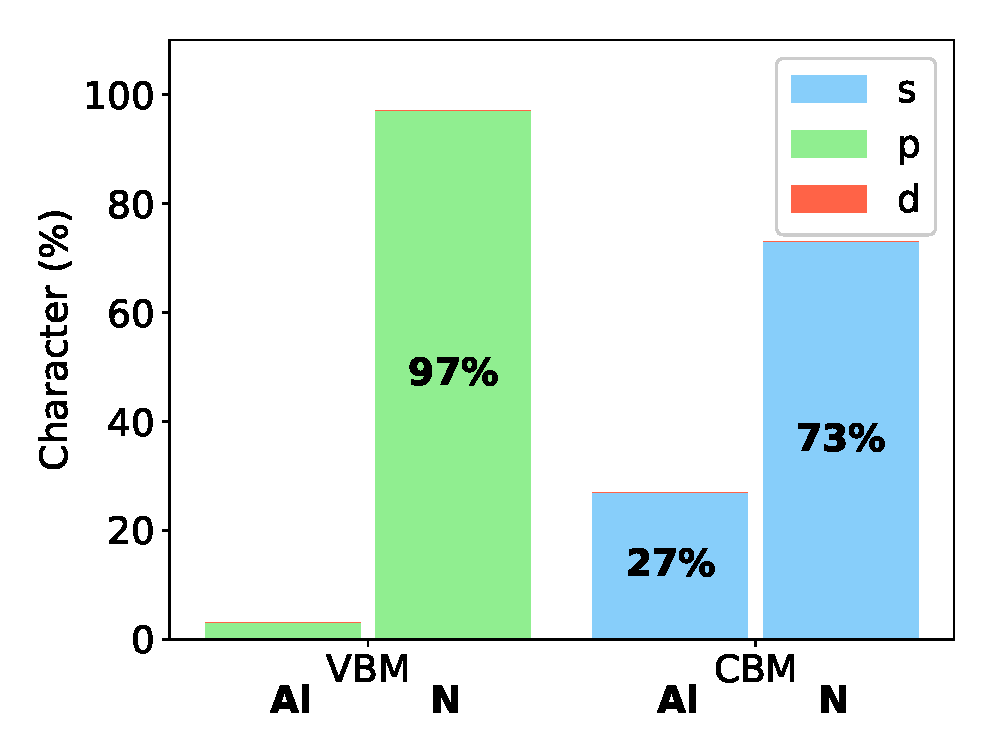
\includegraphics[width=\linewidth]{images/aln_3d_composition.eps}
  \caption{AlN}
\end{subfigure}\hfil % <-- added
\begin{subfigure}{0.3\textwidth}
  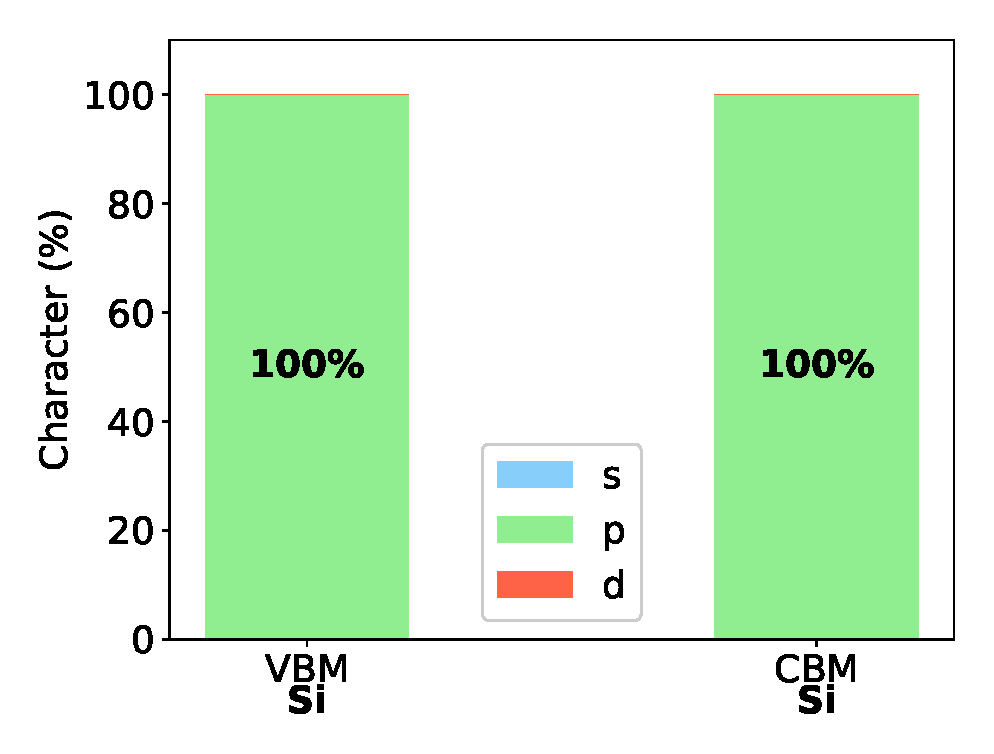
\includegraphics[width=\linewidth]{images/si_3d_composition.eps}
  \caption{Si}
\end{subfigure}
\begin{subfigure}{0.3\textwidth}
  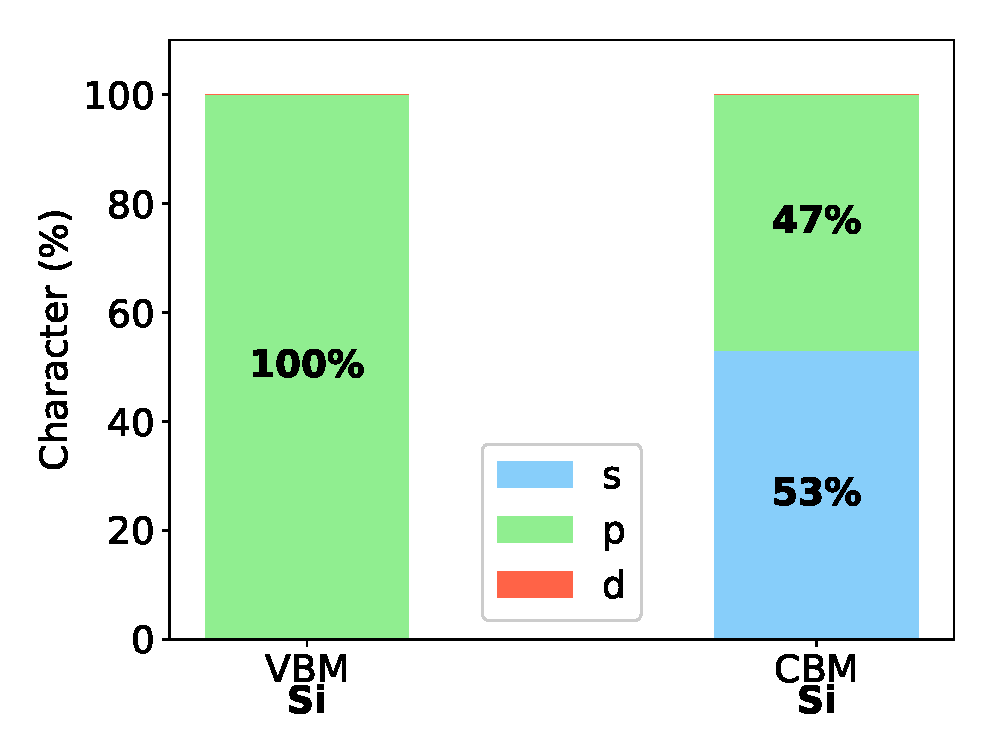
\includegraphics[width=\linewidth]{images/si_indirect_3d_composition.eps}
  \caption{Si indirect}
\end{subfigure}\hfil % <-- added

\medskip

\begin{subfigure}{0.3\textwidth}
  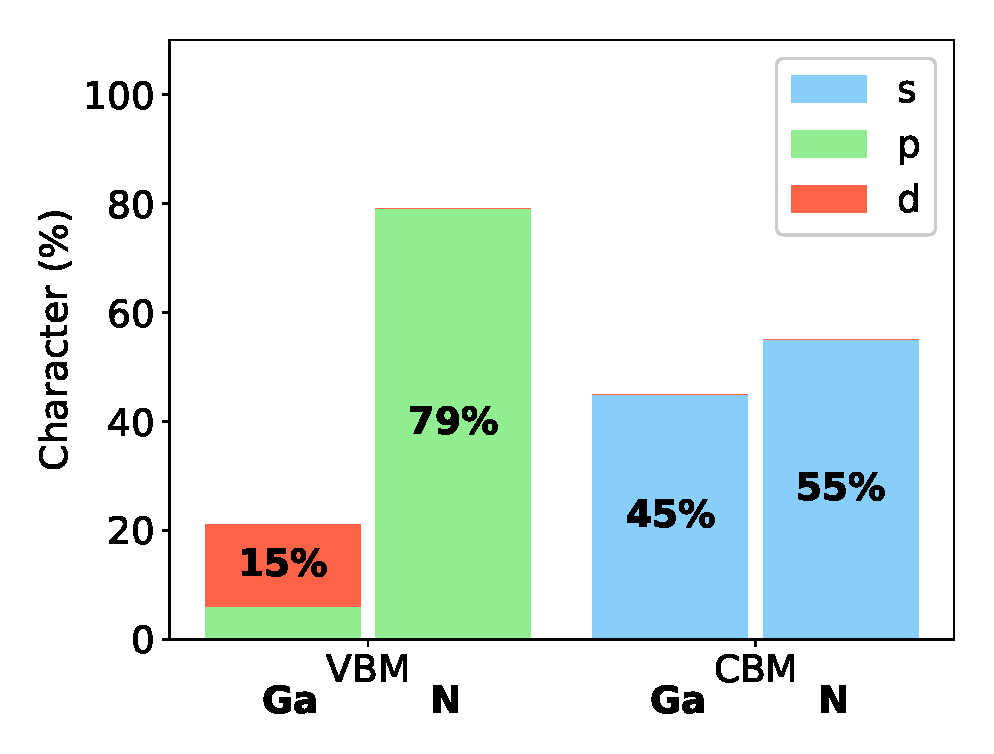
\includegraphics[width=\linewidth]{images/gan_3d_composition.eps}
  \caption{GaN}
\end{subfigure}\hfil % <-- added
\begin{subfigure}{0.3\textwidth}
  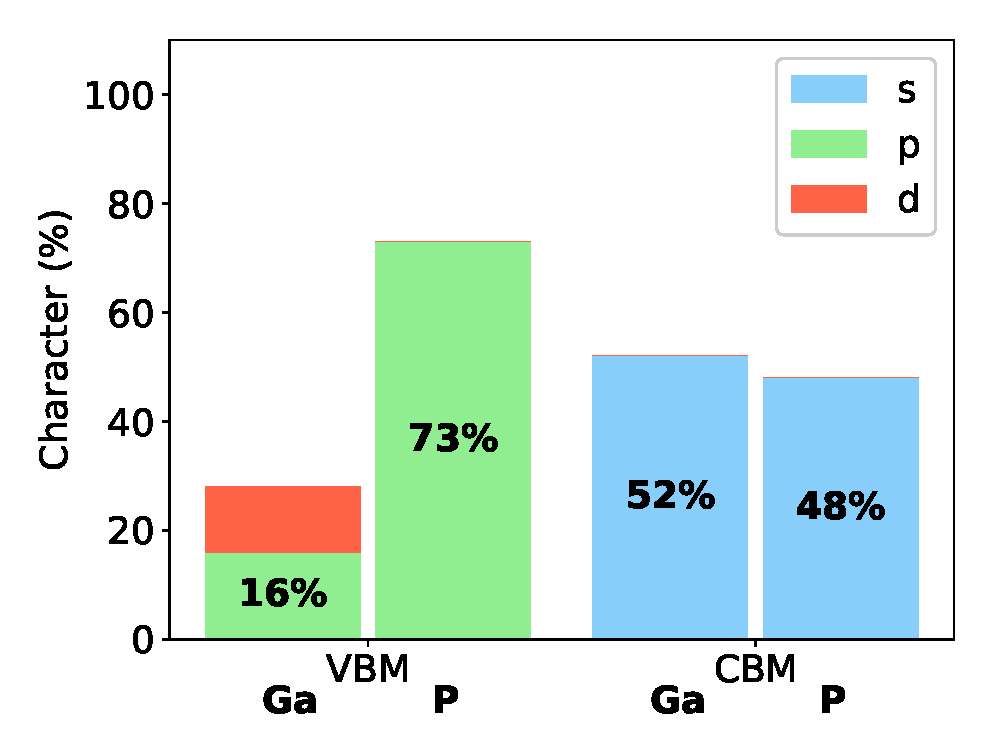
\includegraphics[width=\linewidth]{images/gap_3d_composition.eps}
  \caption{GaP}
\end{subfigure}\hfil % <-- added
\begin{subfigure}{0.3\textwidth}
  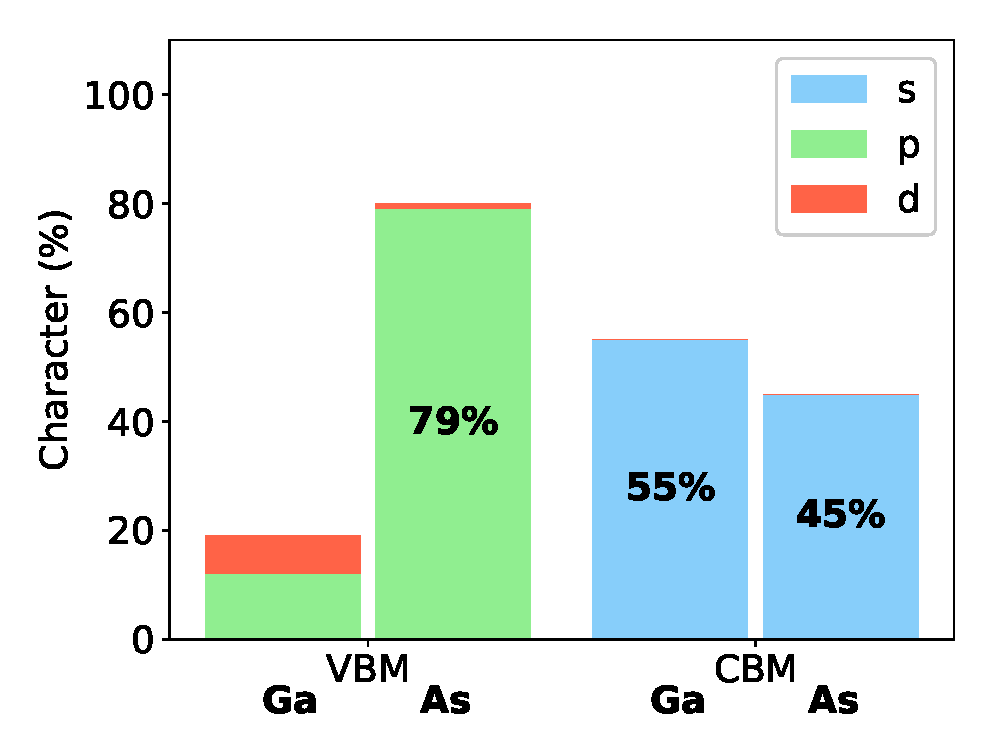
\includegraphics[width=\linewidth]{images/gaas_3d_composition.eps}
  \caption{GaAs}
\end{subfigure}\hfil % <-- added
\medskip
\begin{subfigure}{0.3\textwidth}
  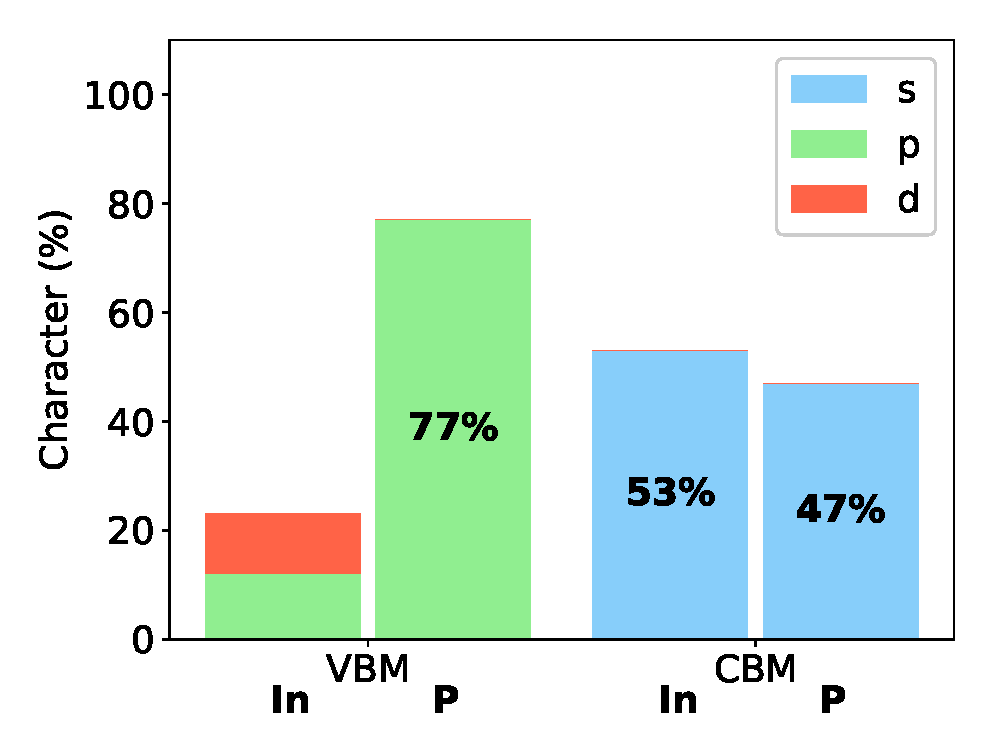
\includegraphics[width=\linewidth]{images/inp_3d_composition.eps}
  \caption{InP}
\end{subfigure}\hfil % <-- added
\begin{subfigure}{0.3\textwidth}
  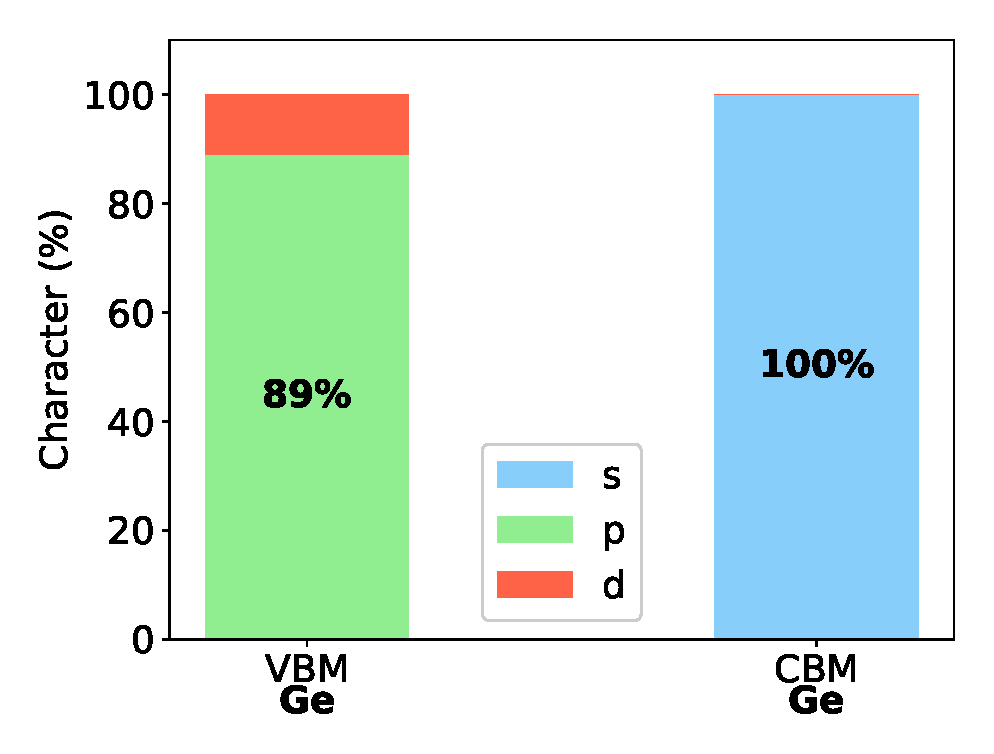
\includegraphics[width=\linewidth]{images/ge_3d_composition.eps}
  \caption{Ge}
\end{subfigure}\hfil % <-- added

        \caption{Composition of the valence band and conduction of three-dimensional compounds. The graph respectively indicates the contribution of s, p, and d orbitals to the character of each band.}
        \label{fig:3d_compounds_character}
\end{figure}

\begin{figure}[!ht]
\centering % <-- added
\begin{subfigure}{0.45\textwidth}
  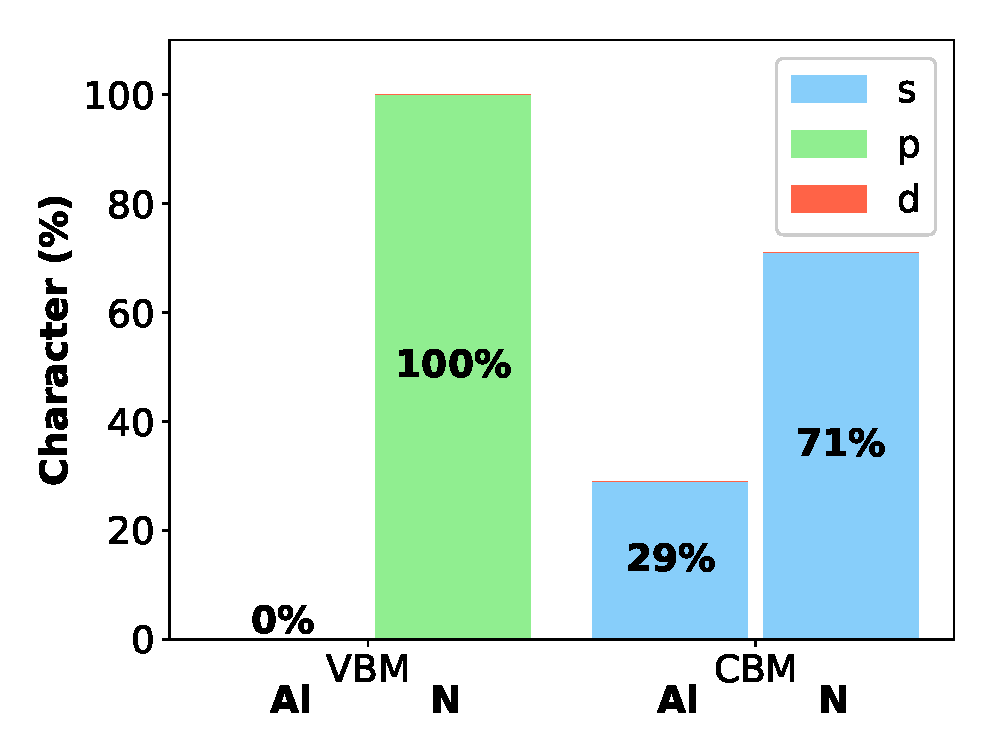
\includegraphics[width=\linewidth]{images/aln_2d_composition.eps}
  \caption{AlN}
\end{subfigure}\hfil % <-- added
\begin{subfigure}{0.45\textwidth}
  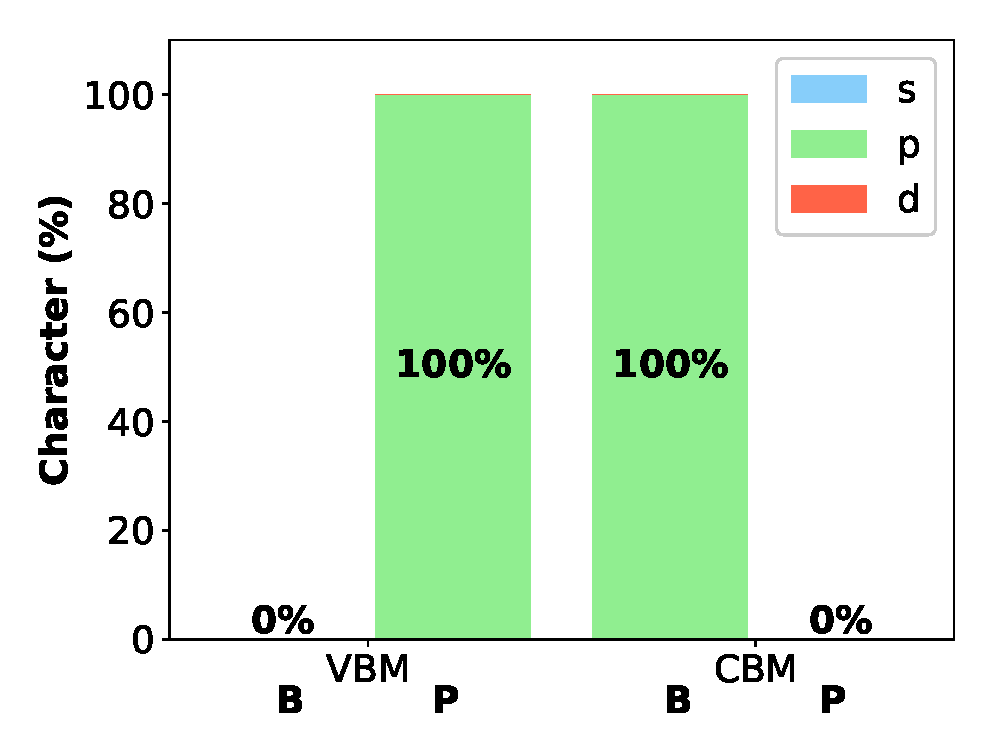
\includegraphics[width=\linewidth]{images/bp_2d_composition.eps}
  \caption{BP}
\end{subfigure}

\medskip

\begin{subfigure}{0.45\textwidth}
  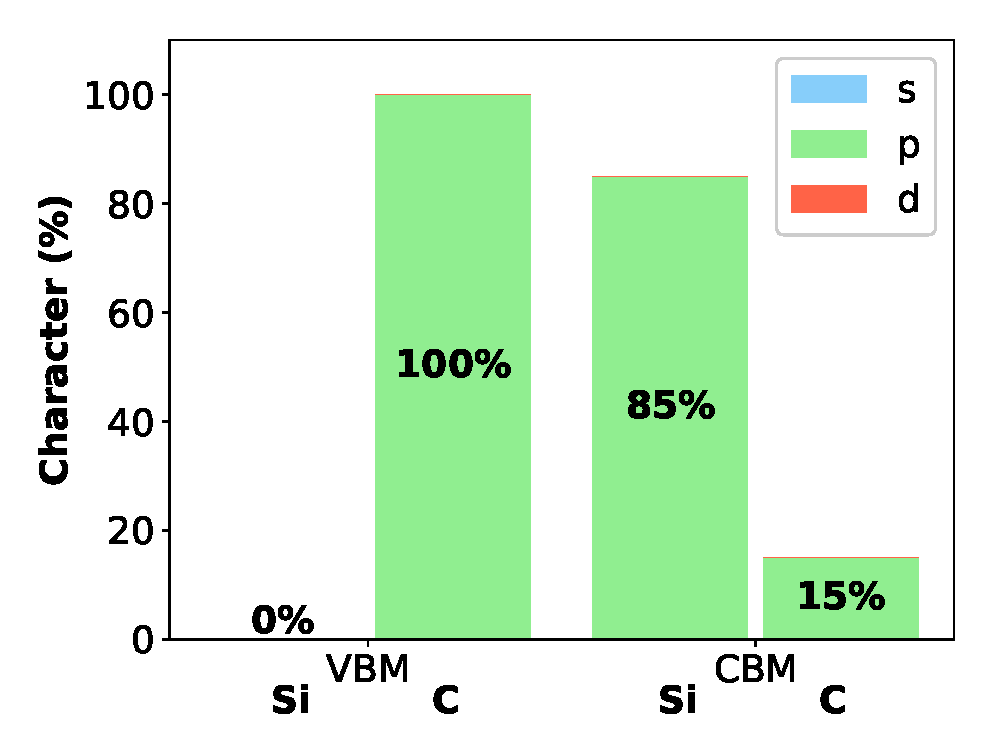
\includegraphics[width=\linewidth]{images/sic_2d_composition.eps}
  \caption{SiC}
\end{subfigure}\hfil % <-- added
\begin{subfigure}{0.45\textwidth}
  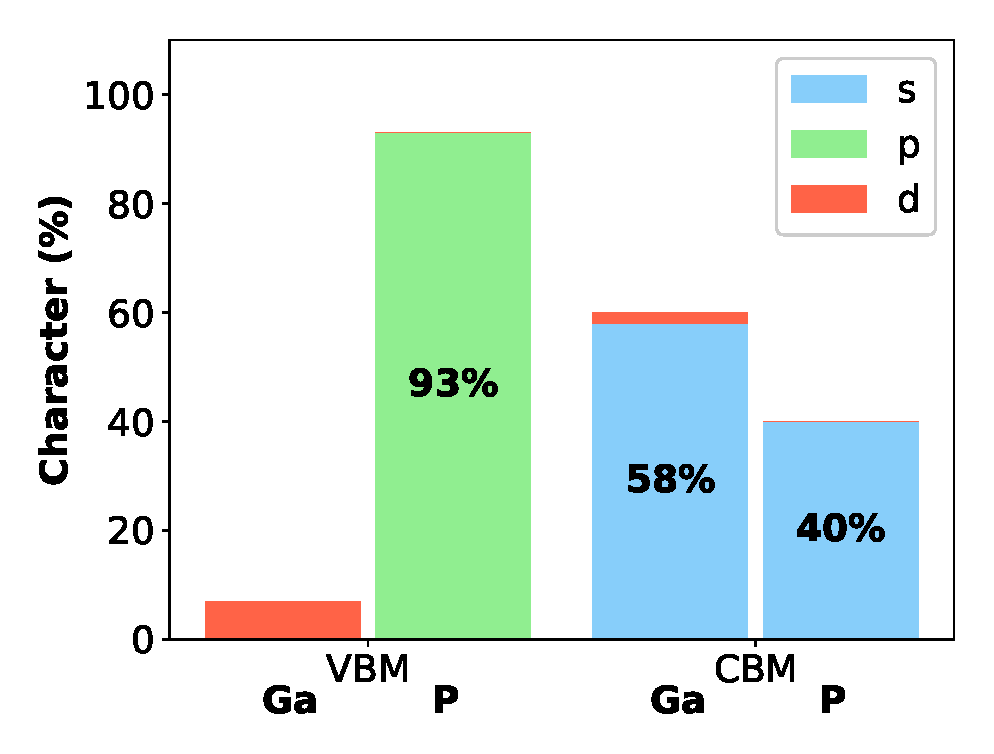
\includegraphics[width=\linewidth]{images/gap_2d_composition.eps}
  \caption{GaP}
\end{subfigure}\hfil % <-- added

\medskip

\begin{subfigure}{0.3\textwidth}
  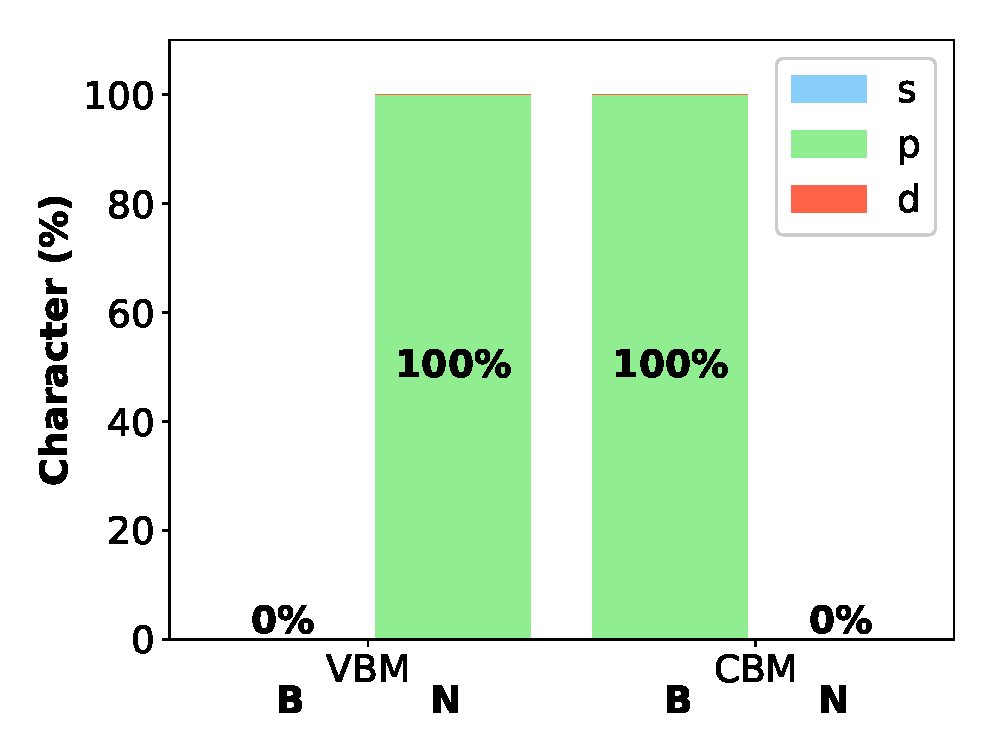
\includegraphics[width=\linewidth]{images/bn_2d_composition.eps}
  \caption{BN}
\end{subfigure}\hfil % <-- added
\begin{subfigure}{0.3\textwidth}
  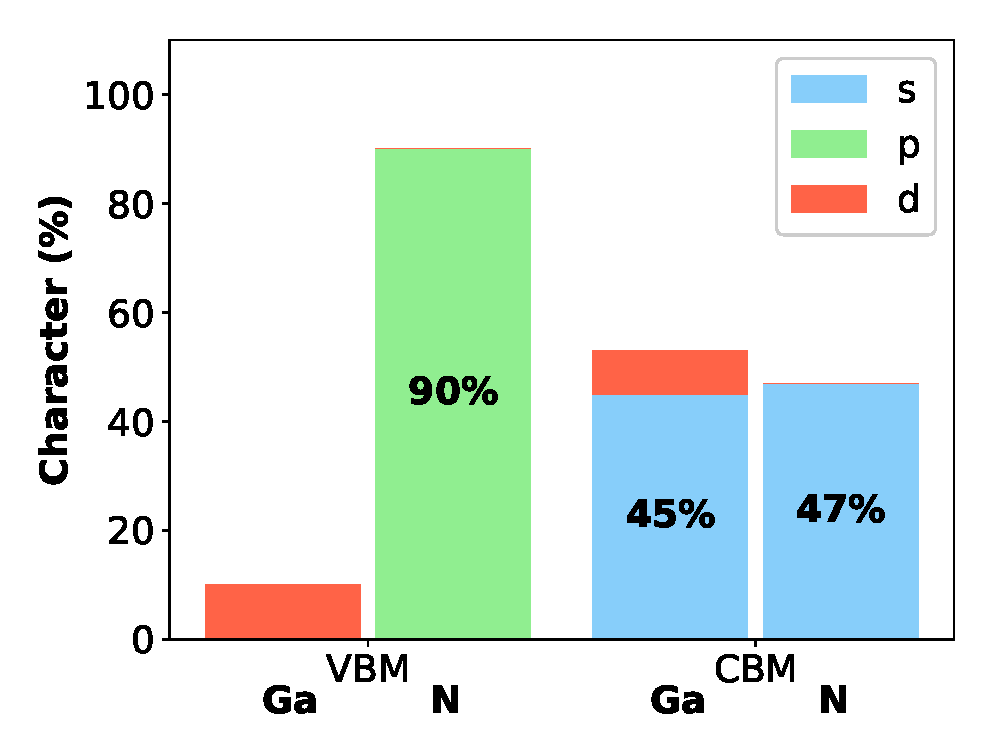
\includegraphics[width=\linewidth]{images/gan_2d_composition.eps}
  \caption{GaN}
\end{subfigure}\hfil % <-- added
\begin{subfigure}{0.3\textwidth}
  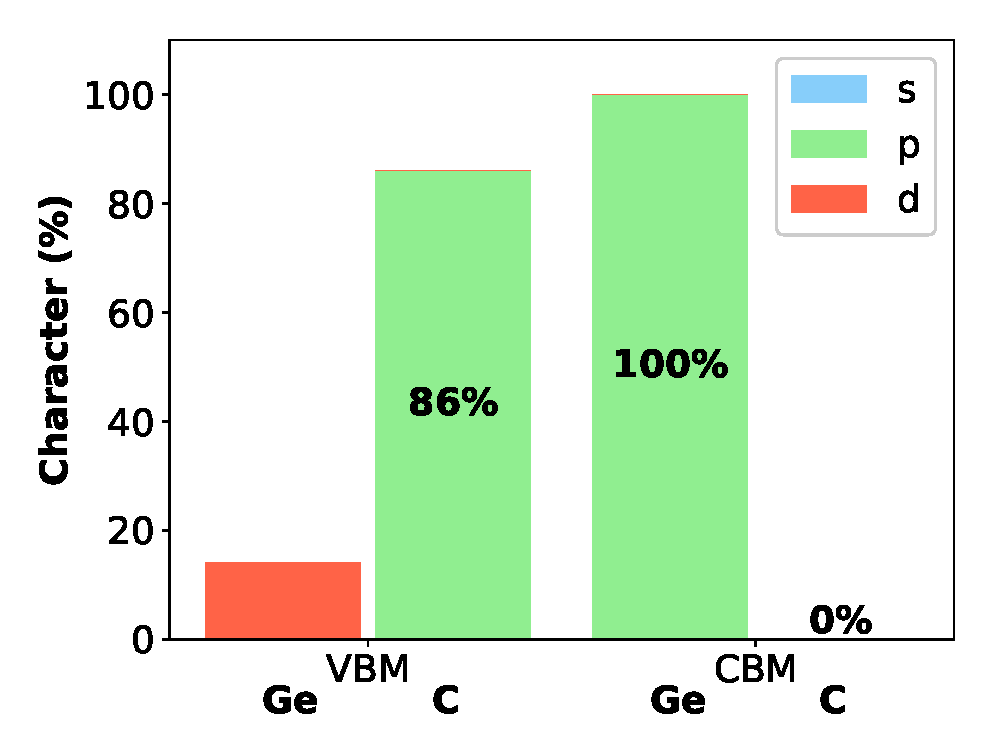
\includegraphics[width=\linewidth]{images/gec_2d_composition.eps}
  \caption{GeC}
\end{subfigure}\hfil % <-- added
        \caption{Composition of the valence band and conduction of two-dimensional compounds. The graph respectively indicates the contribution of s, p, and d orbitals to the character of each band.}
        \label{fig:2d_compounds_character}
\end{figure}
\begin{figure}[!ht]
        \centering
        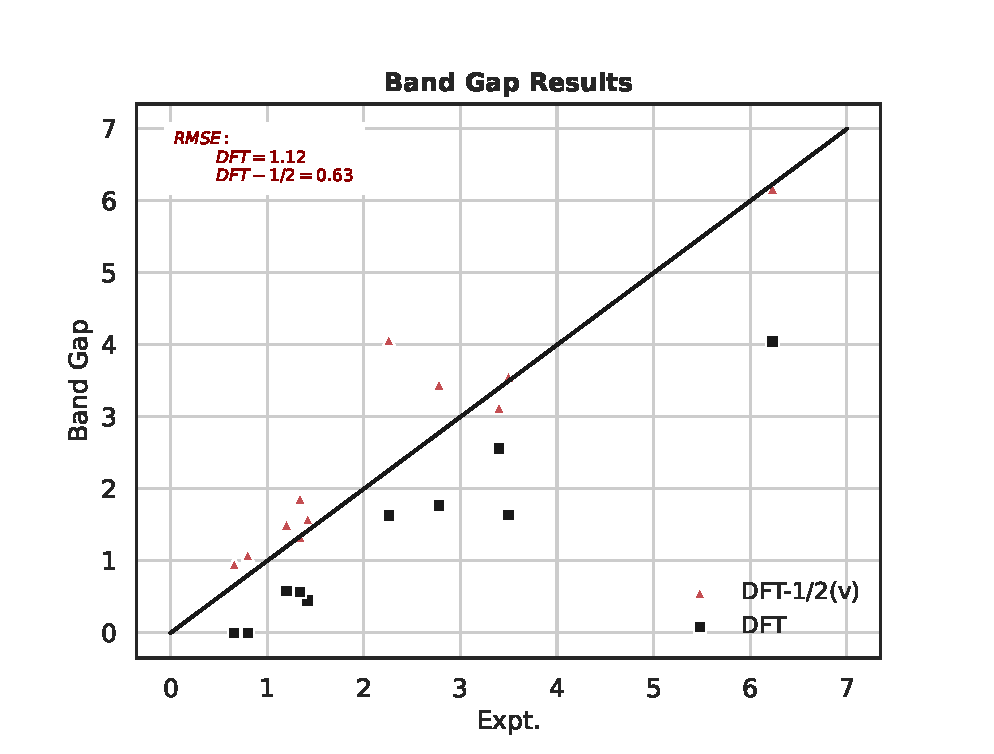
\includegraphics[width=16cm,height=12cm]{images/3d_comparison.eps}
        \caption{Comparison between the experimental values and the obtained values for the three-dimensional materials is presented. The Root Mean Square Error (RMSE) values are also provided for comparing DFT and DFT-1/2, to determine which is closer to the experimental values.}
        \label{fig:3d_comparison}
\end{figure}
\begin{figure}[!ht]
        \centering
        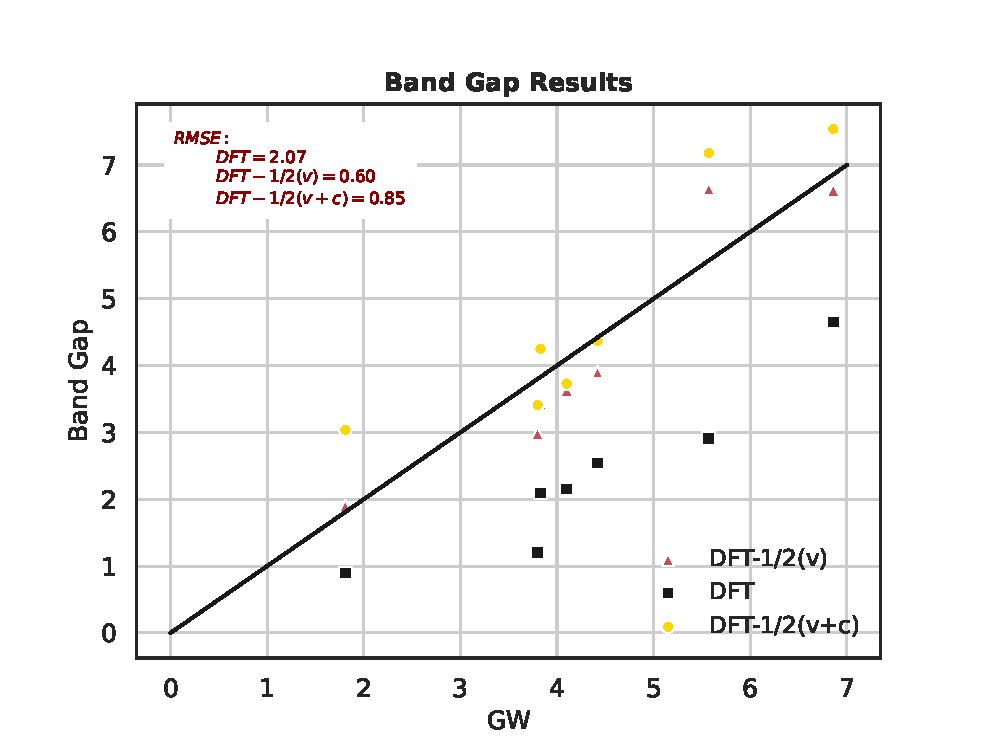
\includegraphics[width=16cm,height=12cm]{images/2d_comparison.eps}
        \caption{Comparison between the GW results and the obtained values for the two-dimensional materials is presented. The Root Mean Square (RMS) values are also provided for comparing DFT, DFT-1/2(v), and DFT-1/2(v+c) .}
        \label{fig:2d_comparison}
\end{figure}

\begin{figure}[!ht]
\centering % <-- added
\begin{subfigure}{0.45\textwidth}
  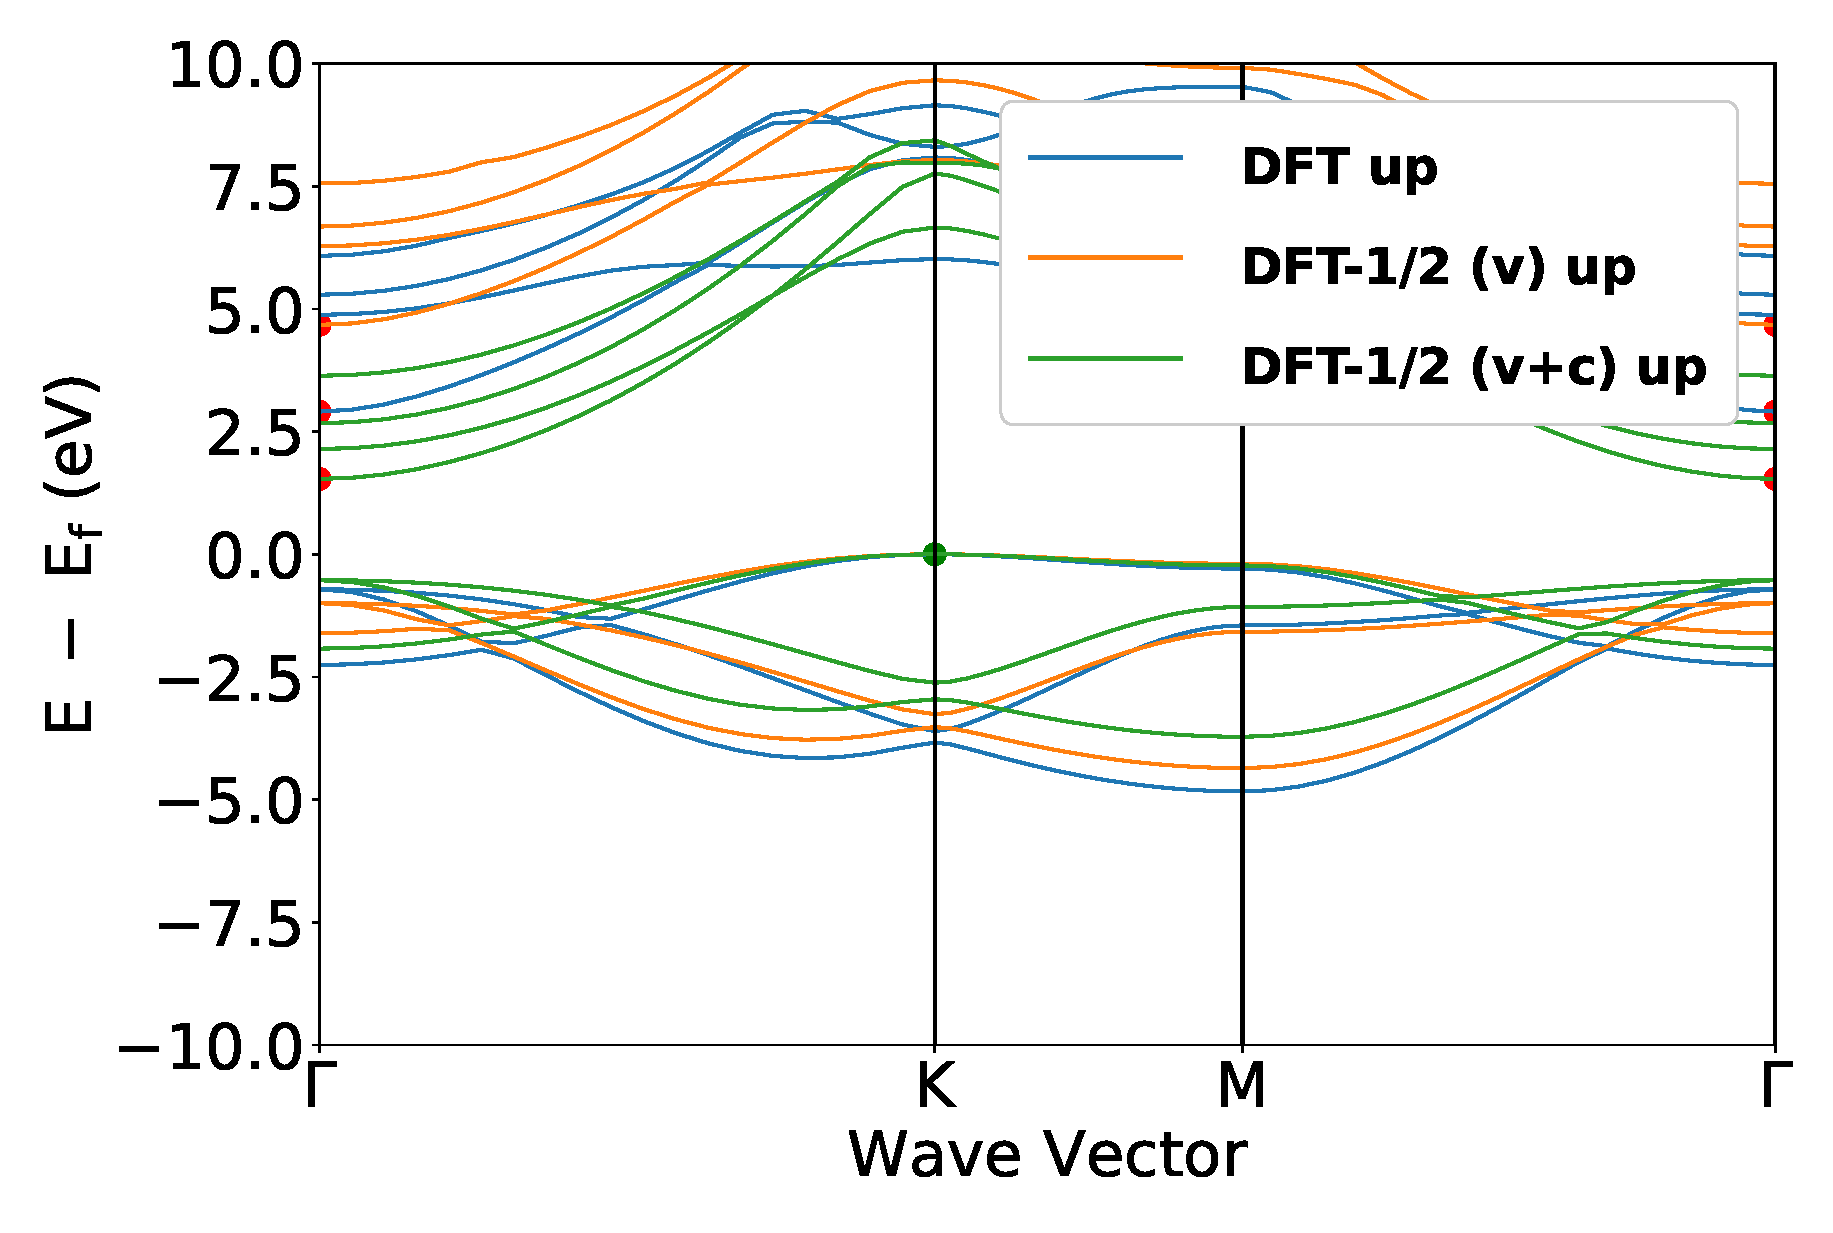
\includegraphics[width=\linewidth]{images/band_2d_aln.eps}
  \caption{AlN}
\end{subfigure}\hfil % <-- added
\begin{subfigure}{0.45\textwidth}
  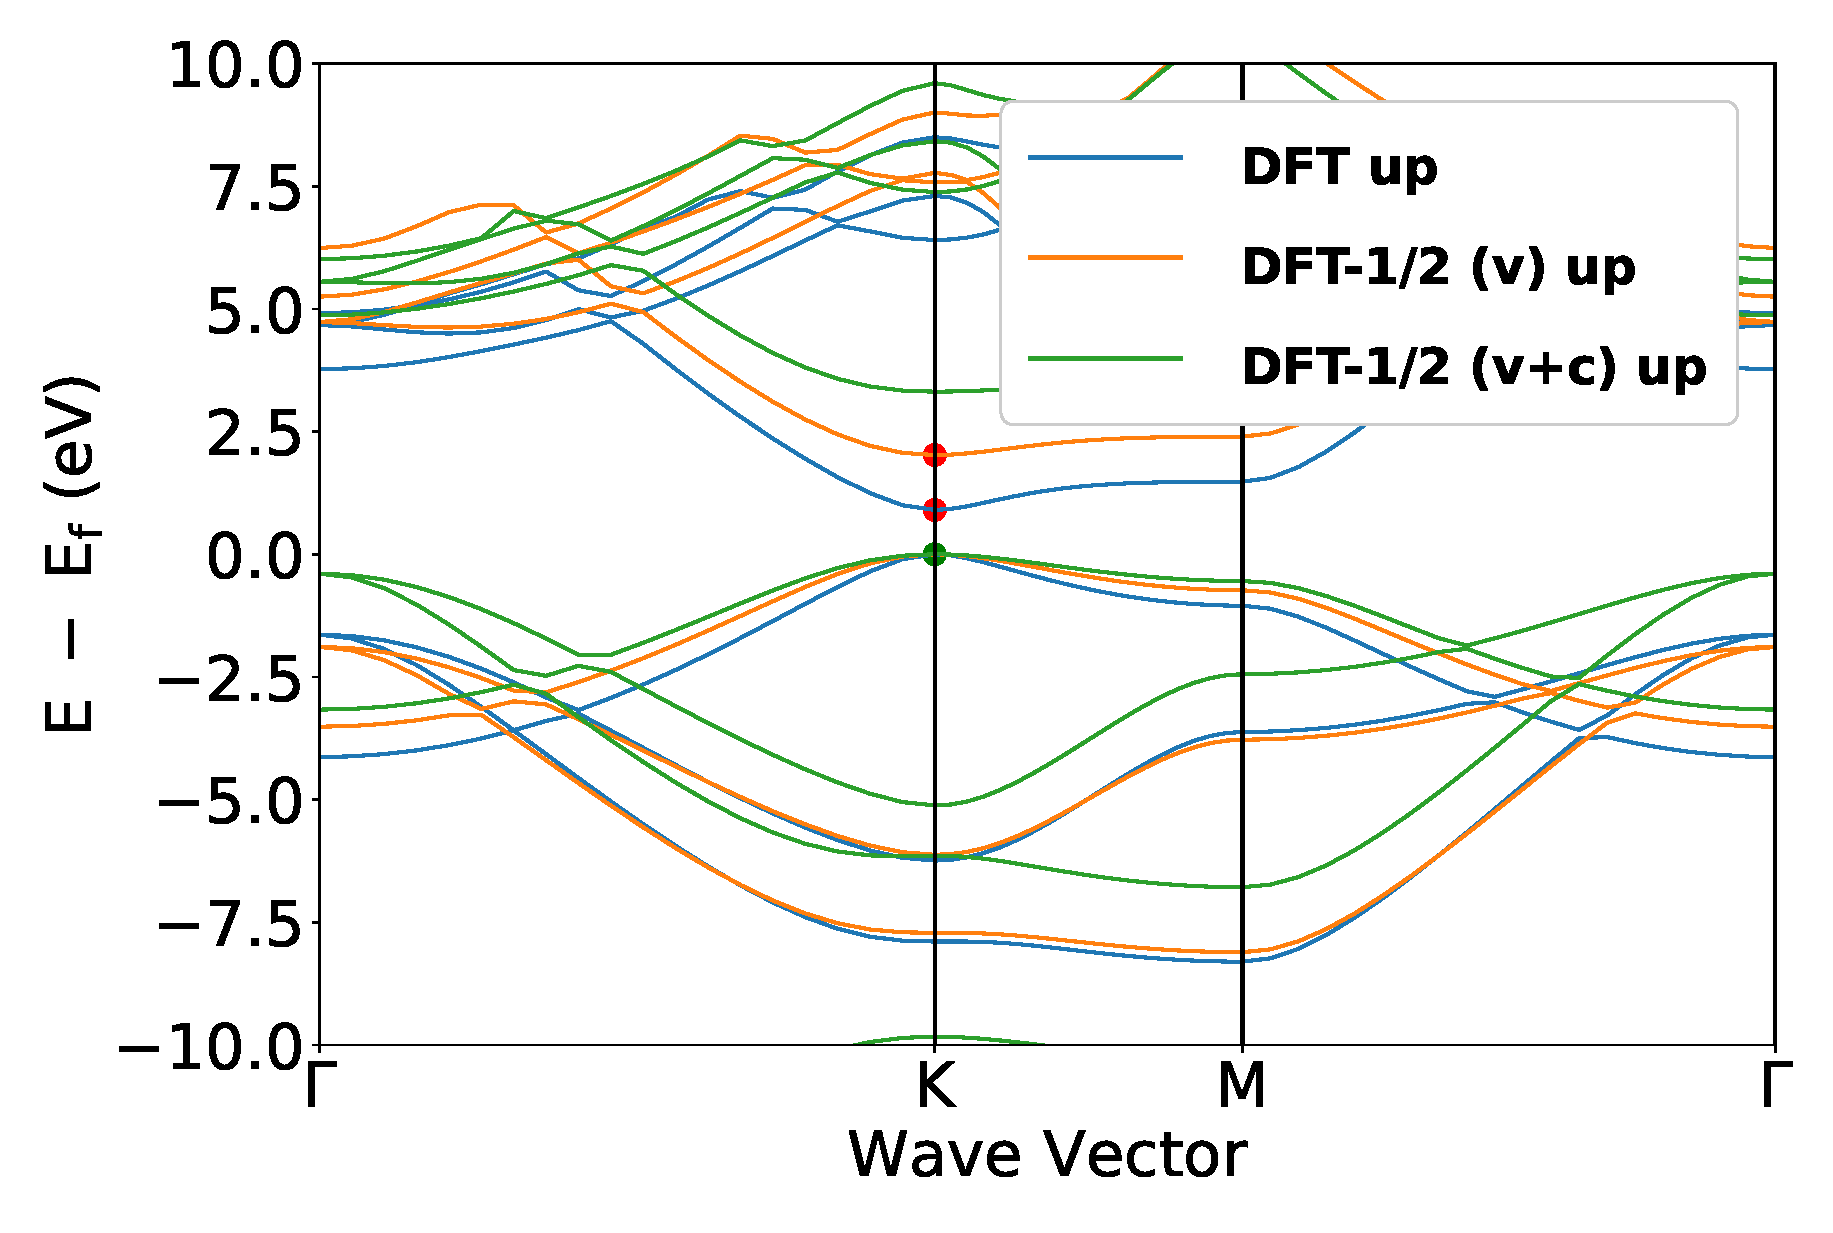
\includegraphics[width=\linewidth]{images/band_2d_bp.eps}
  \caption{BP}
\end{subfigure}

\medskip

\begin{subfigure}{0.45\textwidth}
  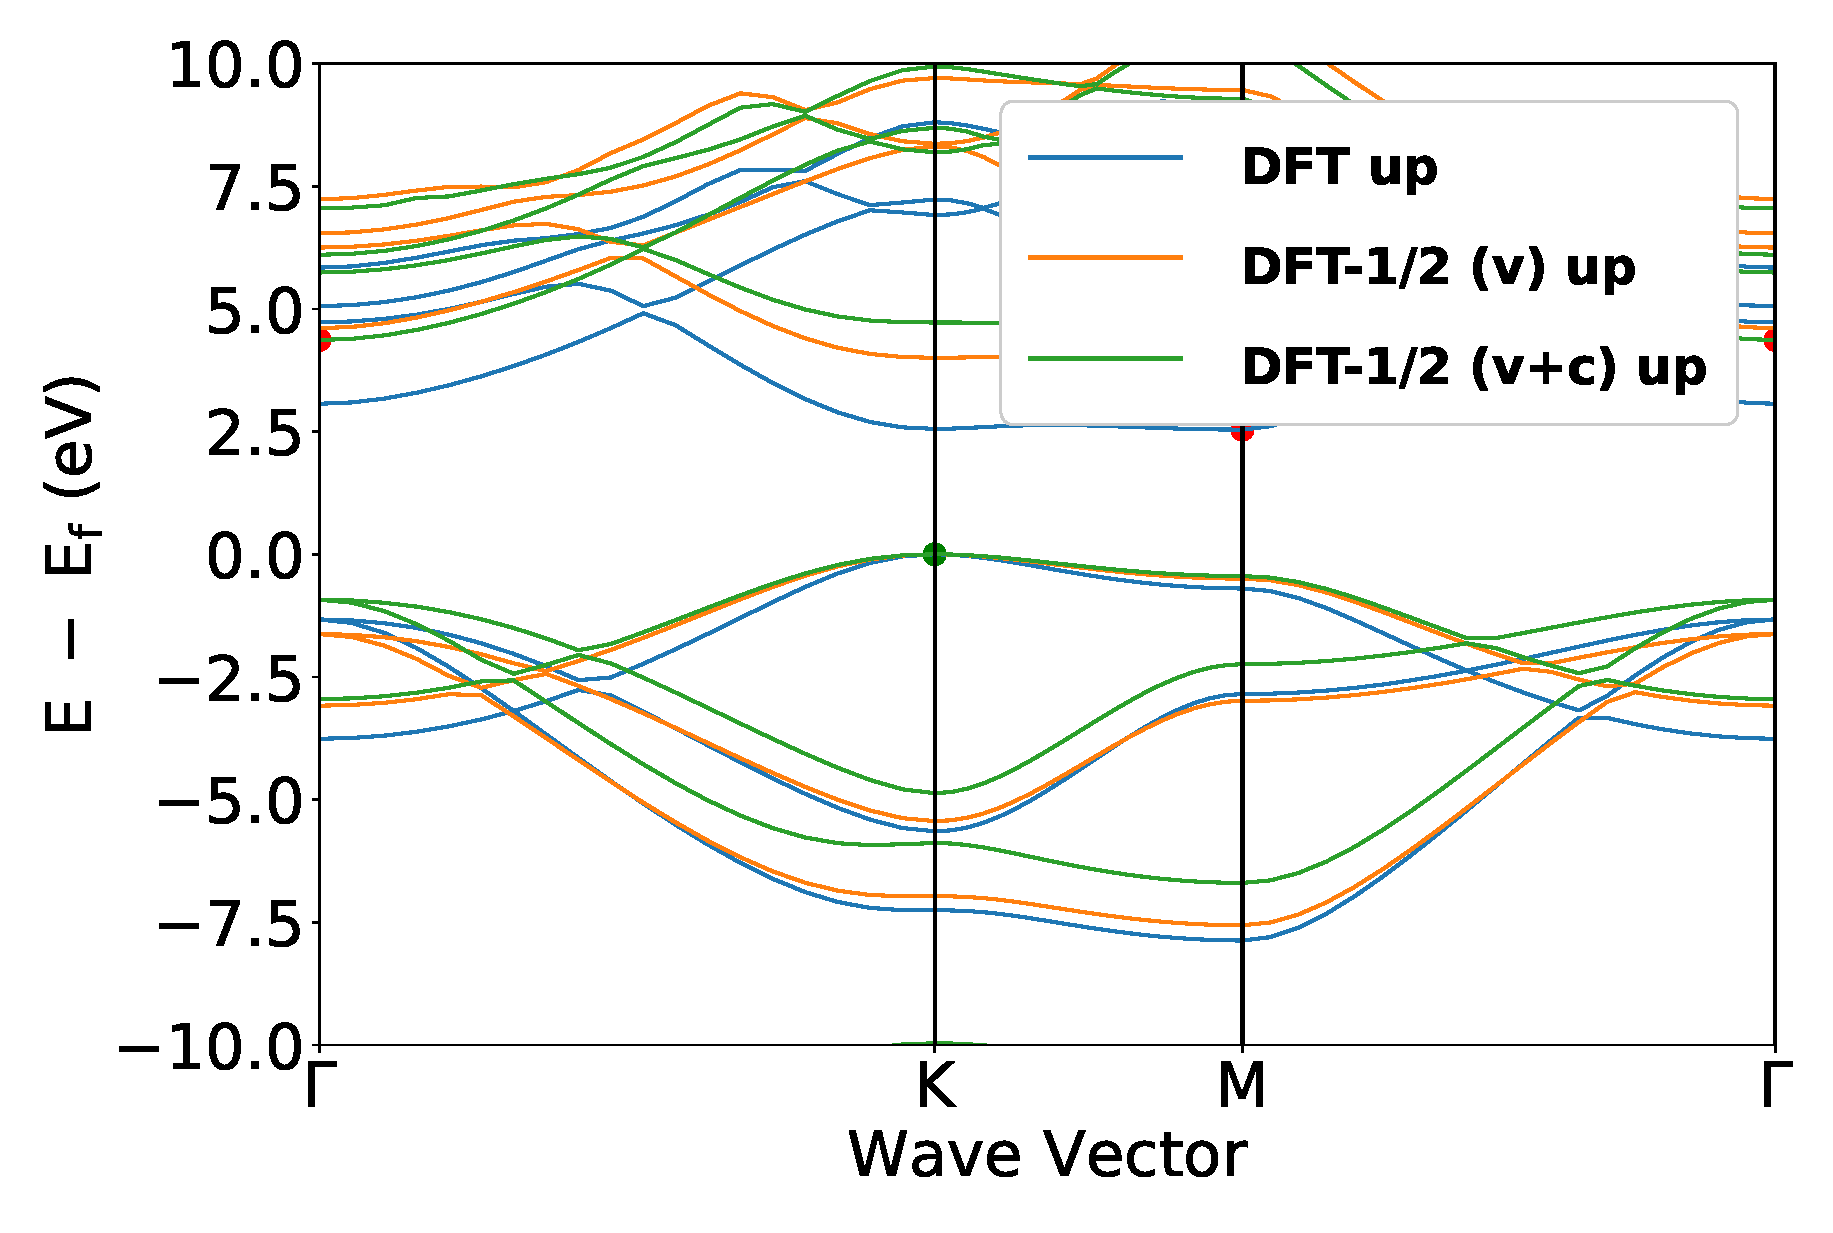
\includegraphics[width=\linewidth]{images/band_2d_sic.eps}
  \caption{SiC}
\end{subfigure}\hfil % <-- added
\begin{subfigure}{0.45\textwidth}
  \includegraphics[width=\linewidth]{images/band_2d_gap.eps}
  \caption{GaP}
\end{subfigure}\hfil % <-- added

\medskip

\begin{subfigure}{0.3\textwidth}
  \includegraphics[width=\linewidth]{images/band_2d_bn.eps}
  \caption{BN}
\end{subfigure}\hfil % <-- added
\begin{subfigure}{0.3\textwidth}
  \includegraphics[width=\linewidth]{images/band_2d_gan.eps}
  \caption{GaN}
\end{subfigure}\hfil % <-- added
\begin{subfigure}{0.3\textwidth}
  \includegraphics[width=\linewidth]{images/band_2d_gec.eps}
  \caption{GeC}
\end{subfigure}\hfil % <-- added
        \caption{Band structure of all 2D elements simulated in this work. In each figure, one has the comparison of the band structure calculated with DFT in relation to the bands calculated with DFT-1/2 using valence and valence-conduction corrections.}
        \label{fig:2d_compounds_bands}
\end{figure}

\begin{figure}[!ht]
\centering % <-- added
\begin{subfigure}{0.45\textwidth}
  \includegraphics[width=\linewidth]{images/band_3d_AlN.eps}
  \caption{AlN}
\end{subfigure}\hfil % <-- added
\begin{subfigure}{0.45\textwidth}
  \includegraphics[width=\linewidth]{images/band_3d_GaAs.eps}
  \caption{GaAs}
\end{subfigure}

\medskip

\begin{subfigure}{0.45\textwidth}
  \includegraphics[width=\linewidth]{images/band_3d_GaN.eps}
  \caption{GaN}
\end{subfigure}\hfil % <-- added
\begin{subfigure}{0.45\textwidth}
  \includegraphics[width=\linewidth]{images/band_3d_GaP.eps}
  \caption{GaP}
\end{subfigure}\hfil % <-- added

\medskip

\begin{subfigure}{0.3\textwidth}
  \includegraphics[width=\linewidth]{images/band_3d_Ge.eps}
  \caption{Ge}
\end{subfigure}\hfil % <-- added
\begin{subfigure}{0.3\textwidth}
  \includegraphics[width=\linewidth]{images/band_3d_InP.eps}
  \caption{InP}
\end{subfigure}\hfil % <-- added
\begin{subfigure}{0.3\textwidth}
  \includegraphics[width=\linewidth]{images/band_3d_Si.eps}
  \caption{Si}
\end{subfigure}\hfil % <-- added
        \caption{Band structure of all 3D elements simulated in this work. In each figure, one has the comparison of the band structure calculated with DFT in relation to the bands calculated with DFT-1/2, employing the appropriate correction for the specific use case.}
        \label{fig:3d_compounds_bands}
\end{figure}